% ──────────────────────────────────────────────────────────────
% Thesis.tex - standard book class
% ──────────────────────────────────────────────────────────────
\documentclass[12pt,a4paper, openany]{book}

% - Encoding & fonts -
\usepackage[utf8]{inputenc}
\usepackage[T1]{fontenc}
\usepackage{lmodern}
\usepackage{microtype}
\usepackage[main=english,french]{babel}

% - Page geometry & headers -
\usepackage[
  a4paper,
  left=2.5cm, right=2.5cm,
  top=2.5cm, bottom=2.5cm,
  headheight=14.5pt   
]{geometry}
\raggedbottom  


% - Line spacing & paragraph -
\usepackage{setspace}
\onehalfspacing
\setlength{\parindent}{0pt}
\setlength{\parskip}{1.5ex}
\usepackage{enumitem}
\setlist[itemize]{leftmargin=1.6em, labelsep=0.5em}

% - Mathematics -
\usepackage{amsmath,amssymb,amsfonts,amsthm}
\newtheorem{proposition}{Proposition}

% - Graphics & floats -
\usepackage{graphicx,svg,float,rotating,longtable}
\usepackage{float}
\usepackage[skip=4pt, belowskip=2pt, aboveskip=4pt]{caption}
\setlength{\intextsep}{0pt plus 2pt minus 2pt}
\captionsetup{
  % font=small,
  font=footnotesize,
  labelfont=bf,
  textfont=normalfont,
  skip=0.25cm,
  justification=justified
}

% type-specific overrides:
\captionsetup[table]{position=above}
\captionsetup[figure]{position=below}
\usepackage{booktabs,tabularx,multirow}
\newcolumntype{Y}{>{\centering\arraybackslash}X}
\usepackage{siunitx}

% - Bibliography & hyperlinks -
\usepackage[colorlinks,allcolors=blue]{hyperref}
\usepackage[authoryear,round]{natbib}
\setcitestyle{citesep={,}}

% - Index & todos -
\usepackage{makeidx}
\makeindex
\usepackage[colorinlistoftodos,textsize=scriptsize]{todonotes}

\usepackage{fancyhdr,lastpage}

% Roman-numbered frontmatter:
\fancypagestyle{frontmatterstyle}{%
  \fancyhf{}%
  \fancyhead[L]{\slshape\rightmark}%
  \fancyhead[R]{\thepage}%
  \renewcommand{\headrulewidth}{0.5pt}%
}

% Arabic-numbered mainmatter:
\fancypagestyle{mainmatterstyle}{%
  \fancyhf{}%
  \fancyhead[L]{\slshape\rightmark}%
  \fancyhead[R]{page~\thepage~(of~\pageref{LastPage})}%
  \renewcommand{\headrulewidth}{0.5pt}%
}

% set the default to frontmatter style:
\AtBeginDocument{\pagestyle{frontmatterstyle}}
\let\cleardoublepage\clearpage


% ──────────────────────────────────────────────────────────────
% Document
% ──────────────────────────────────────────────────────────────
\begin{document}
\frontmatter
% \title{Portfolio Construction with Gaussian Mixture Models}
% \author{
%   Ivan Khalin\\
%   \href{mailto:ivan.khalin@unil.ch}{ivan.khalin@unil.ch}
% }
% \date{May, 2025}
% \maketitle


\begin{titlepage}
  \vspace*{4.5cm}
  \centering
  {\LARGE\bfseries Portfolio Construction with Gaussian Mixture Models\par}
  \vspace{1.5cm}

  {\Large Ivan Khalin\par}
  \vspace{0.2cm}
  {\small\href{mailto:ivan.khalin@unil.ch}{ivan.khalin@unil.ch}\par}
  \vspace{0.2cm}
  {\small June, 2025\par}
  \vspace{1cm}

  {\small MSc in Finance, University of Lausanne\par}
  {\small Supervisor: Marc-Aurèle Divernois\par}
  {\small Expert: Madhushree Ayalasomayajula\par}
  \vspace{2cm}

  \vfill
  {\footnotesize\textbf{Disclaimer:}\par
  The work is the responsibility of the author; in no way does it engage the responsibility of the University, nor of the supervising Professor.\par}

\end{titlepage}
\chapter*{Abstract}
\addcontentsline{toc}{chapter}{Abstract}
\begin{otherlanguage}{english}
In this paper, we review and implement the portfolio construction technique using Gaussian mixture models as described by \cite{luxenbergPortfolioConstructionGaussian2022}. To complement the original study, we conduct a preliminary empirical analysis of this approach. We also explore a related method based on kernel density estimation. The first section explains the mathematical foundations of both models. The second section presents a comparative empirical analysis, in which we narrow down optimal configurations and assess the practical viability of each approach.
\end{otherlanguage}

\vspace{3ex}

\phantomsection
\begin{otherlanguage}{french}
    Dans ce mémoire, nous examinons et implémentons la technique de construction de portefeuille basée sur les modèles de mélanges gaussiens, telle que décrite par \cite{luxenbergPortfolioConstructionGaussian2022}. Afin de compléter l'étude originale, nous réalisons une analyse empirique préliminaire de cette approche. Nous explorons également une méthode apparentée utilisant l'estimation par noyaux. La première partie expose les fondements mathématiques des deux modèles. La seconde présente une analyse empirique comparative, au sein de laquelle nous identifions les configurations optimales et évaluons la viabilité pratique de chaque approche.
\end{otherlanguage}

\vfill
% \vspace{1em}
  \textbf{Keywords:} Asset Allocation; Portfolio Choice; Semiparametric Methods; Financial Econometrics.\\
  \textbf{JEL Classification:} G11; C14; C58

\chapter*{Executive Summary}
\addcontentsline{toc}{chapter}{Executive Summary}

Because equity returns are skewed and heavy-tailed, Harry Markowitz's Gaussian mean-variance optimization systematically understates downside risks. Despite extensive empirical evidence of these return characteristics, the mean-variance framework remains popular due to its analytical clarity and closed-form tractability. Existing approaches to incorporate skewness, such as behavioral utility frameworks or Mean-Variance-Skewness-Kurtosis (MVSK) models, either rely on subjective parameters, non-rational investor biases, or sacrifice the elegance and computational efficiency inherent in Markowitz's original model.

This thesis addresses a key research question: \textit{Can skewness be embedded into portfolio optimization without introducing subjective parameters, sacrificing convexity, or relying on restrictive functional forms?} We benchmark Gaussian Mixture Models (GMM), a recent parametric method, and propose Kernel Density Estimation (KDE) as a fully non-parametric enhancement. Both approaches replace the single-Gaussian assumption by approximating returns as weighted sums of Gaussian components.

Methodologically, substituting these densities into exponential utility maximization yields a log-sum-exponent (LSE) objective. This LSE formulation adaptively amplifies the weighting of downside scenarios proportional to the traditional risk-aversion parameter $\gamma$. Critically, this preserves convexity, ensuring computational efficiency and global optimality while embedding skewness directly into the portfolio optimization process.

Empirically, the density-based strategies were tested across four major equity indices (S\&P500, FTSE100, EURO STOXX50, Hang Seng) over the period 2015-2025. We evaluated a large configuration space of 828 stable configurations varying in frequency, lookback windows, rebalancing intervals, and universe sizes. Key findings include:

\begin{itemize}
    \item Three distinct investment regimes emerged based on the risk aversion parameter $\gamma$: (1) Return-seeking regime ($\gamma<\bar{\gamma}$) closely resembling standard Markowitz solutions; (2) Variance-floor regime ($\gamma=\bar{\gamma}$) characterized by a modified minimum-variance portfolio; and (3) Skew-seeking regime ($\gamma>\bar{\gamma}$), willingly accepting higher volatility to pursue positive skewness.
    \newpage
    \item KDE portfolios consistently demonstrate superior stability and competitive risk-adjusted returns compared to GMM portfolios. Particularly in turbulent markets and short-window configurations ($\leq$12 months), KDE outperformed classical Markowitz portfolios in 59\% of cases on a risk-adjusted basis, delivering an average penalized Sharpe ratio improvement of 12\%, while outperforming MAR across the board on downside risk measures.
    \item GMM showed attractive in-sample results but suffered from substantial performance dispersion out-of-sample and won fewer than 15\% of cases. GMM's computational intensity, driven by the Expectation-Maximization procedure, outweighed its practical benefits.
\end{itemize}

This thesis contributes to the literature by demonstrating that integrating skewness through density estimation maintains both rational decision-making foundations and analytical clarity. The proposed KDE-based method requires minimal tuning, solely involving the familiar risk-aversion parameter, and significantly enhances downside risk management.

Practically, KDE provides an intuitive, theoretically grounded bridge between classical mean-variance optimization and the empirical reality of skewed financial returns. Future research directions include incorporating transaction costs, testing null-bandwidth KDE across all configurations, extending adaptive LSE weighting to risk-parity portfolios, and evaluating the method's robustness in high-frequency contexts.

\chapter*{Acknowledgements}
\addcontentsline{toc}{chapter}{Acknowledgements}

I am deeply grateful to Marc-Aurèle Divernois for his guidance and encouragement throughout this project. His insightful feedback and readiness to discuss ideas were invaluable at every stage.

My thanks also go to the team at the CEDIF data centre for their efficient help in obtaining and preparing the market and constituent data that underpin the empirical analysis.
\tableofcontents
\listoftables
\listoffigures

%----------------------------------------------------------------
\mainmatter
\pagestyle{mainmatterstyle}
\chapter{Introduction}
\label{chap:intro}
\lhead{Chapter 1. \emph{Introduction}}

Harry Markowitz's mean-variance approach gave us the elegant intuition for the trade-off between expected return and volatility. This lesson, however, was predicated on the assumption that asset returns are normally (or at least elliptically) distributed. Empirical studies have long demonstrated that returns exhibit skewness and heavy tails, features that the Gaussian model cannot accommodate. Ignoring these higher-order characteristics leads to systematic underestimation of downside risk and mispricing of asymmetric payoffs.

From early surveys of capital budgeting to recent evidence of skewness-seeking in hedge-fund allocations (\cite{maoSurveyCapitalBudgeting1970}, \cite{benuzziSkewnessseekingBehaviorFinancial2024}), the fact that investors care deeply about asymmetry has been thoroughly attested to. Practitioners routinely favor portfolios whose return distributions offer the potential for infrequent large gains, even at the cost of modest increases in variance. It follows that any model that aspires to capture realistic market prices must account for skewness. 

Embedding skewness directly via non-Gaussian densities quickly sacrifices the analytical clarity of the mean-variance framework. Once returns follow, for instance, a skewed Student-$t$ distribution, closed-form expressions for portfolio moments vanish and must be estimated by numerical integration or simulation. Despite offering performance benefits, optimization under these densities becomes a computationally intensive black box, obscuring the intuitive "risk-return" trade-off.

A natural alternative approach is to focus on embedding skewness into the utility function rather than the distribution itself. However, as \cite{ebertSkewnessPreferencePopularity2016} demonstrate, skewness preferences are incompatible with classical expected utility theory (EUT). This "impossibility result" states that no smooth, concave expected-utility function can display a strong preference for skewness. Intuitively, a Taylor expansion around any wealth level demonstrates that the first-order (mean) and second-order (variance) effects cancel out when you introduce an infinitesimal skew in probabilities, leaving only a third-order term. Hence, in the immediate neighborhood of any reference wealth, expected utility is effectively blind to small skew shifts: it treats a tiny chance of a large gain just the same as a tiny chance of a large loss.

One way of avoiding this limitation of EUT is to adopt behavioral utility models. Two main extensions to EUT have enabled the modeling of skewness: Rank-Dependent Expected Utility (RDEU) and Cumulative Prospect Theory (CPT) (\cite{quigginTheoryAnticipatedUtility1982}, \cite{tverskyAdvancesProspectTheory1992}). RDEU extends EUT using a Probability Weighting Function (PWF) to inflate the perceived likelihood of tail events. CPT builds on RDEU by introducing separate value and PWFs for gains versus losses. These modifications allow for skewness-seeking on the upside to differ from skewness-aversion on the downside, which RDEU cannot model (\cite{kligerTheoriesChoiceRisk2009}). 

These utility models do provide a better descriptive account of how real assets are priced. This success, however, hinges on incorporating the non-rationality of human decision making into the utility framework. Indeed, the way in which a financial decision is made and the way it should be made are two distinct questions. In other words, a prudent investor ought to assess whether a rational decision and a decision that maximizes the utility function that captures their biases are one and the same. It is thus unsurprising that applications of behavioral utility frameworks to portfolio construction show a general trend of underperformance compared to classical methods. For instance, in \cite{cuiDecisionMakingCumulative2024}, a CPT-based strategy attained considerably lower risk-return characteristics than the equally-weighted portfolio. Furthermore, as \cite{luxenbergPortfolioOptimizationCumulative2024} point out, CPT-based optimization is computationally challenging, and analytical solutions have as of yet been devised only for approaches with considerable axiomatic limitations. 

An alternative way of incorporating skewness is by means of Mean-Variance-Skewness-Kurtosis models (MVSK), initially proposed by \cite{konnoMeanVarianceSkewnessPortfolioOptimization1995}. These models have thoroughly demonstrated their ability to offer performance advantages over the traditional methods, as \cite{mandalHigherorderMomentsPortfolio2024} summarize. However, the MVSK framework relies on ad hoc parametrization of skewness (kurtosis) preference (aversion) parameters. Additionally, any single skewness metric conflates tail weight and tail distance and thus cannot, on its own, distinguish different forms of asymmetry. These shortcomings of MVSK models, coupled with the computational challenges and the lack of analytical insights, leave much to be desired in terms of interpretability.

To reconcile tractability with a faithful representation of asymmetry, we return to the density-based introduction of higher moments. Gaussian Mixture Models (GMMs) provide a natural first step toward flexible density estimation. By representing the return distribution as a weighted sum of Gaussian components, GMMs can approximate a wide array of shapes, while allowing us to preserve an "MV-style" interpretation of optimal solutions. The conceptual groundwork for the use of GMM in portfolio construction was laid by \cite{luxenbergPortfolioConstructionGaussian2022}, and later expanded upon by \cite{wangRobustContextualPortfolio2022}. Building on these, this thesis tests GMM-based portfolios across five major equity indices, and with a broader configuration space than the previous works. Our out-of-sample findings diverge from those of the second paper, for reasons we will analyze in Chapter~\ref{chap:empirical}.

More importantly, we introduce a kernel-density (KDE) variant that eliminates the computationally heavy tuning step inherent in GMM, and show that this non-parametric alternative delivers markedly superior stability. KDE "lets the data speak" by placing a smooth kernel at each observed return, automatically capturing any degree of skewness or tail-fatness without specifying functional forms. In Chapter~\ref{chap:math}, we detail the mathematical foundations of GMM and KDE. Then, in Chapter~\ref{chap:portfolio}, we derive portfolios under each estimator, establish their convexity, and interpret the resulting analytical insights. Finally, in Chapter~\ref{chap:empirical}, we present a comparative empirical analysis of these methods, provide guidance for practitioners, and discuss future research directions.

\chapter{Mathematical Preliminaries}
\label{chap:math}
\lhead{Chapter 2. \emph{Mathematical Preliminaries}}

The discussion in this section draws primarily on \cite{KernelDensityEstimators2015} and \cite{OtherApplications2015}, which develop the theory of KDE and GMMs, respectively, except where other sources are noted. We begin by introducing the KDE approach, from which GMM follows easily. These preliminaries establish the mathematical foundation for the portfolio construction techniques in Chapter~\ref{chap:portfolio}.

\section{Kernel Density Estimation}
\subsection{Univariate Case}
\label{sec:univkde}

Suppose we observe a vector of $n$ realizations $X=(x_1,x_2,...,x_n)$ of a random variable $x$. We wish to obtain a continuous density function $\hat{f_h}(x)$ based on this empirical set of observations, without making any further assumptions about the underlying distribution. 

A kernel function $K(x)$ is typically a non-negative, integrable function for which $\int K(x)dx = 1$. The kernel estimate associates with each observation $x_i$ a scaled kernel function $K_h(x)$. Each kernel acts as a localized smoothing function centered at $x_i$. The bandwidth parameter $h$ governs the dispersion of the kernel around each observation, thereby influencing the smoothness of the estimated density $\hat{f_h}(x)$. The scaled kernel function is defined as:
$$\displaystyle K_h(x)=\frac{1}{h}K\left(\frac{x}{h}\right)$$
where the factor $1/h$ ensures that $\hat{f_h}(x)$ is properly scaled. If $K(x)$ is a valid density function, this scaling ensures that $\hat{f_h}(x)$ integrates to 1 over its domain.

The final density $\hat{f_h}(x)$ is then defined as the sum of the scaled kernel functions $K_h(x)$, centered at each observation $x_i$:
$$\displaystyle\hat{f_h}(x)=\frac{1}{n}\sum_{i=1}^{n}K_h(x-x_i)=\frac{1}{nh}\sum_{i=1}^{n}K\left(\frac{x-x_i}{h}\right)$$

The selection of the kernel function $K(x)$ is an active area of research. For our analysis, the Gaussian kernel is a natural choice, given how well it integrates with the exponential utility function. This property will be required when we derive the moments for portfolio construction in Section \ref{sec:momentsec}. An individual Gaussian kernel is given by:
$$\displaystyle K(x)=\frac{1}{\sqrt{2\pi}}\exp\left(-\frac{1}{2}x^2\right)$$

Typically, in KDE, the bandwidth $h$ plays the role of a dispersion parameter, similar to the standard deviation in a normal distribution. It then follows that the kernel density estimate with a Gaussian kernel is:
$$\displaystyle\hat{f_h}(x)=\frac{1}{n}\sum_{i=1}^{n}\frac{1}{h\sqrt{2\pi}}\exp\left(-\frac{1}{2}\left(\frac{x-x_i}{h}\right)^2\right)$$

The quality of a density estimator can be assessed pointwise by its mean squared error (MSE), which decomposes into variance and bias squared:
$$
\mathrm{MSE}\bigl[\hat f(x)\bigr]
= \mathbb{E}\bigl[\hat f(x)-f(x)\bigr]^2
= \mathrm{Var}\bigl[\hat f(x)\bigr] + \bigl(\mathrm{Bias}[\hat f(x)]\bigr)^2,
$$
where
$$
\mathrm{Bias}[\hat f(x)]
= \mathbb{E}[\hat f(x)] - f(x),
$$
and $f(x)$ is the true, unknown distribution of $x$.

Since we care about the entire density surface, we next integrate this pointwise error over $x$ to obtain the integrated squared error (ISE):
$$
\mathrm{ISE}
= \int \bigl[\hat f(x)-f(x)\bigr]^2\,dx.
$$
Taking the expectation of ISE across all samples yields the mean integrated squared error (MISE):
$$
\mathrm{MISE}
= \mathbb{E}[\mathrm{ISE}]
= \int \mathbb{E}\bigl[\hat f(x)-f(x)\bigr]^2\,dx
= \int \mathrm{MSE}\bigl[\hat f(x)\bigr]\,dx.
$$

MISE provides a single global criterion that balances bias and variance. The choice of $h$ is what controls this tradeoff:

\begin{itemize}
\item As $h\downarrow0$, $\hat f_h$ bias tends to zero, but the variance is inflated.
\item As $h\uparrow\infty$, $\hat f_h$ the estimator collapses toward a flat density, resulting in low variance and high bias.
\end{itemize}

An optimal $h$ minimizes MISE, but since the true underlying distribution $f(x)$ is unknown, we cannot compute MISE directly. In practice, we approximate MISE minimization via methods such as cross-validation, as discussed below (\ref{sec:crossval}).

\begin{figure}[H]
  \begin{center}
  \begin{minipage}{\textwidth}
    \centering
    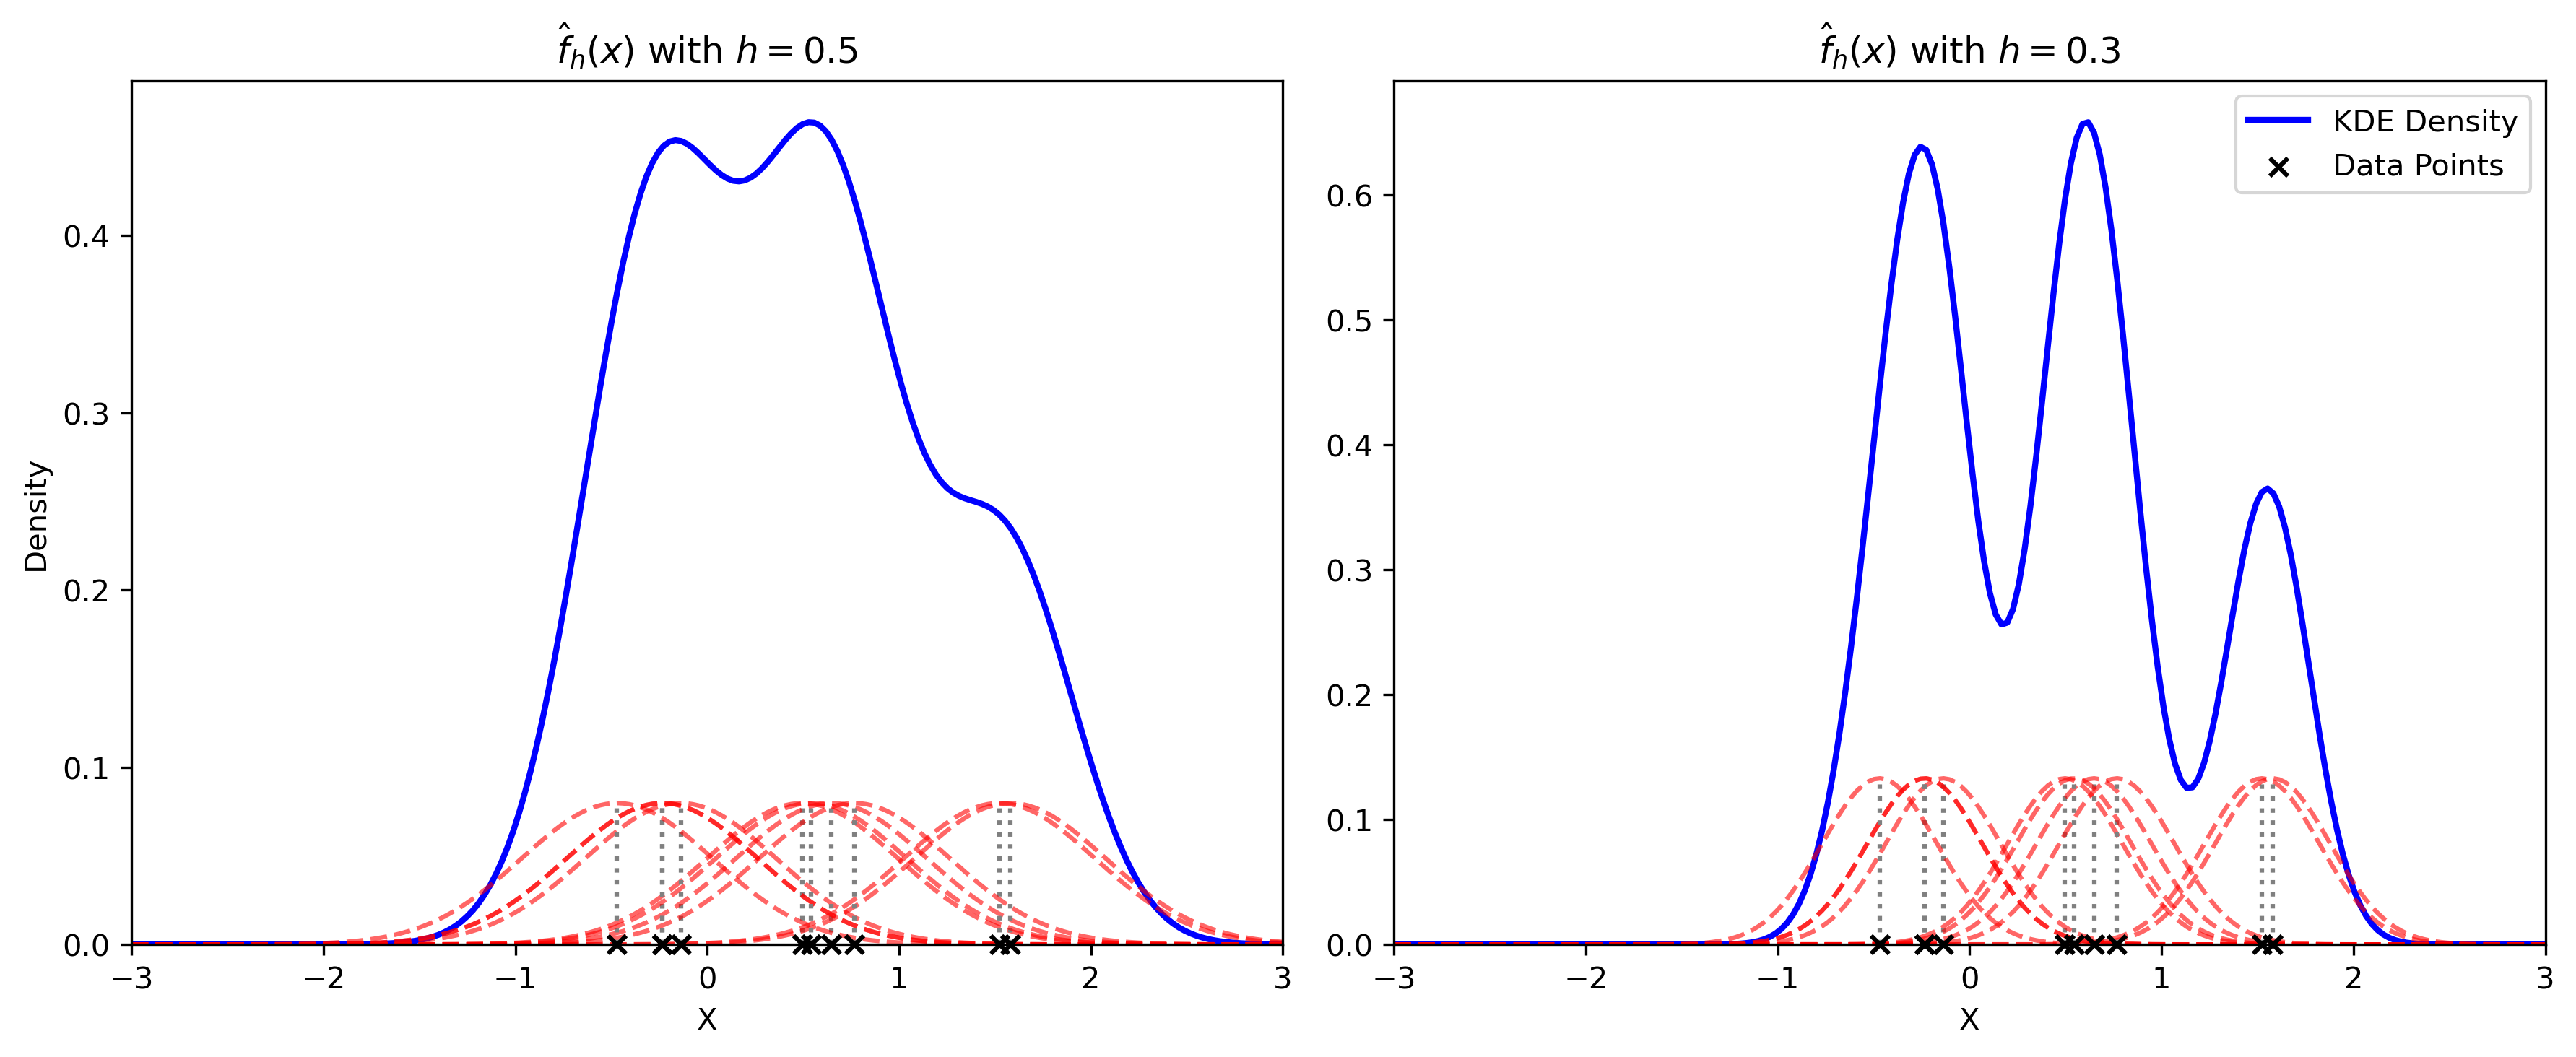
\includegraphics[width=\textwidth]{images/20_1.png}
  \end{minipage}
  \hfill
  \caption[Effect of bandwidth on KDE densities]{Higher bandwidth $h$ results in smoother density estimates. KDE from $n=5$ standard-normal draws, using Gaussian kernels with $h=0.5$ (left) and $h=0.3$ (right). Solid blue curves are the summed densities; dashed red curves are the individual kernels at each observation (black $\times$), and dotted vertical lines mark $\pm h$ around each point. A smaller $h$ preserves multimodal peaks, while a larger $h$ yields a smoother, lower-amplitude estimate.}
  \label{fig:combined1}
  \end{center}
  \end{figure}
The above makes it clear that a Gaussian kernel density estimator is nothing more than a sum of scaled Gaussians. This is a convenient opportunity to illustrate how the shape of $\hat{f_h}(x)$ varies as the bandwidth $h$ varies. Figure \ref{fig:combined1} demonstrates a set of 5 fictitious observations drawn from a standard normal distribution. Each observation is associated with a red Gaussian kernel, and the resulting blue density estimator is the sum of these kernels. Notably, a lower bandwidth results in a distinctly multimodal density, whereas a higher value of $h$ attenuates these peaks.
  


\subsection{Multivariate Case}

KDE also allows us to model multivariate empirical distributions, with the intuition remaining unchanged from the univariate case. Suppose we observe $n$ vectors $\mathbf{x}_i=(x_{i1}, x_{i2},...,x_{id})^\mathsf{T}$, where each vector is an observation drawn from an unknown $d$-variate distribution. The entire set of observations can be written as the matrix $\mathbf{X}=(\mathbf{x}_1,\mathbf{x}_2,...,\mathbf{x}_n)^{\mathsf{T}}\in\mathbb{R}^{n\times d}$. To estimate the probability density, we evaluate the kernel density estimator at a query point $\mathbf{x}=(x_{1}, x_{2},...,x_{d})\in\mathbb{R}^{d}$.

The multivariate KD estimator is thus defined in terms of some multivariate kernel function $K_\mathbf{H}(\mathbf{x})$ and $\mathbf{H}$ is the $d\times d$ symmetric positive definite bandwidth matrix:
$$\displaystyle\hat{f_h}(\mathbf{x})=\frac{1}{n}\sum_{i=1}^{n}K_\mathbf{H}(\mathbf{x}-\mathbf{x}_i)$$
Where $K_\mathbf{H}(\mathbf{x})$ is the scaled kernel function $K(\mathbf{x})$, so that:
$$\displaystyle K_\mathbf{H}(\mathbf{x})=\frac{1}{\sqrt{\det{(\mathbf{H})}}}K(\mathbf{{H}^\mathrm{-1/2}x})$$
When the Gaussian kernel is used, the KDE density is defined as:
$$\displaystyle\hat{f_h}(\mathbf{x})=\frac{1}{n}\sum_{i=1}^{n}\frac{1}{(2\pi)^{d/2}\sqrt{\det{(\mathbf{H})}}}\exp\left(-\frac{1}{2}\mathbf{(x-x_{\it{i}})^\mathsf{T}H^\mathrm{-1}(x-x_{\it{i}})}\right)$$

The bandwidth matrix $\mathbf{H}$ plays a role analogous to a covariance matrix, controlling the shape, orientation, and spread of the kernel functions. Its parametrization is arguably even more critical than the choice of the kernel. Three common configurations exist:

\begin{enumerate}
\item \textbf{Full bandwidth}: The most flexible form, which allows KDE to capture variations in dispersion and directional dependencies through the off-diagonal terms:
$$\mathbf{H}_{full}=\begin{pmatrix}h^2_1 & h_{12} & \cdots & h_{1d} \\ h_{12} & h^2_2 & \cdots & h_{2d} \\ \vdots & \vdots & \ddots & \vdots \\ h_{1d} & h_{2d} & \cdots & h^2_d\end{pmatrix}$$
This flexibility comes at the cost of increased complexity, requiring estimation of $d(d+1)/2$ parameters, which is feasible in lower dimensions but challenging as $d$ grows.

\item \textbf{Diagonal bandwidth}: A simplification that ignores covariance-like dependence, but still allows for heterogeneous dispersion across the $d$ random variables: 
$$\mathbf{H}_{diagonal}=\begin{pmatrix}h^2_1 & 0 & \cdots & 0 \\ 0 & h^2_2 & \cdots & 0 \\ \vdots & \vdots & \ddots & \vdots \\ 0 & 0 & \cdots & h^2_d\end{pmatrix}=\text{diag}(h^{2}_{1}, ..., h^{2}_{d})$$

\item \textbf{Isotropic bandwidth}: which imposes a uniform dispersion on every kernel with no explicit dependence:
$$\mathbf{H}_{isotropic}=\begin{pmatrix}h^2 & 0 & \cdots & 0 \\ 0 & h^2 & \cdots & 0 \\ \vdots & \vdots & \ddots & \vdots \\ 0 & 0 & \cdots & h^2\end{pmatrix}=h^2I$$
\end{enumerate}

There exist even more elaborate specifications of the bandwidth matrix $\mathbf{H}$, including bandwidth matrices specific to each observation $\mathbf{x}_i$, but we do not discuss these in the context of KDE. Crucially, a KDE estimator does not necessarily rely on the bandwidth matrix to model variable dependence. Instead, dependence arises naturally from the summation of kernels placed over observed data points. A visual example of this will be provided in Section \ref{sec:compare}.

Although the isotropic bandwidth may seem overly simplistic, it can be sufficient for constructing continuous density functions. A full bandwidth may be preferable when KDE is used for clustering, which is not our objective. For the subsequent portfolio analysis, we will use the diagonal bandwidth matrix.



\subsection{Bandwidth Selection via Cross-Validation}
\label{sec:crossval}
The quality of a KDE estimator is sensitive to the choice of the bandwidth matrix, and there are numerous methods for doing so algorithmically. We focus on cross-validation, which allows us to select each $h_i$ by maximizing the log-likelihood of estimators fit on subsets of the data over a fine grid of candidate values.

Concretely, for each random variable $i$ we partition its $n$ observed realizations $\{x_{1},...,x_{n}\}$ into $k$ disjoint folds, and denote by $I_{c}$ the set of indices in fold $c$. For each candidate bandwidth $h$ we then compute the cross-validated score
$$
\mathrm{CV}(h)=
\frac{1}{k}
\sum_{c=1}^{k}
\sum_{j \,\in\, I_c}
\log\left(\hat{f}_{-c,h}(x_j)\right),
$$
Where $\hat{f}_{-c,h}$ denotes the KDE fitted on all data except those in fold $c$, using bandwidth $h$. We then set
$$
\hat{h}_i = 
\arg\max_h\;\mathrm{CV}(h).
$$

In preliminary experiments across our five index universes, each $\hat{h}_i$ aligned almost exactly with the sample standard deviation $\sigma_i$ of the corresponding realization series. To reduce computational time, we therefore fix $\mathbf{H}=\mathrm{diag}\bigl(\sigma_{1}^{2}, \dots, \sigma_{d}^{2}\bigr)$ for all subsequent empirical tests.

\section{Moments}
\label{sec:momentsec}
We will need the mean and variance of a portfolio projection $\mathbf{\alpha^{\mathsf{T}}x}$ under a KDE density (useful in \ref{sec:tangency}). To derive these, working with the moment-generating function (MGF) is convenient. We fix a weight vector $\alpha\in\mathbb R^d$ and let
$$
Y=\alpha^{\mathsf{T}} X,\quad
\hat f(x)=\frac1n\sum_{i=1}^n\mathcal N(x\mid x_i,H).
$$
The moment-generating function of $Y$ is simply the sum of the MGFs of the Gaussian density
$$
M(u)=\mathbb E[e^{uY}]
=\int \exp\bigl(u\,\alpha^{\mathsf{T}} X\bigr)\,\hat f(x)\,dx
=\frac1n\sum_{i=1}^n\exp\!\Bigl(u\,\alpha^{\mathsf{T}} x_i+\tfrac12\,u^2\,\alpha^{\mathsf{T}} H\,\alpha\Bigr).
$$
Taking the first derivative, and evaluating at $u=0$:
$$
M'(u)
=\frac1n\sum_{i=1}^n
\exp\!\Bigl(u\,\alpha^{\mathsf{T}} x_i+\tfrac12\,u^2\,\alpha^{\mathsf{T}} H\,\alpha\Bigr)
\Bigl(\alpha^{\mathsf{T}} x_i+u\,\alpha^{\mathsf{T}} H\,\alpha\Bigr).
$$
$$
M'(0)
=\frac1n\sum_{i=1}^n(\alpha^{\mathsf{T}} x_i)
=\alpha^{\mathsf{T}}\bar x.
$$
Thus:
$$\mathbb{E}[\alpha^{\mathsf{T}} X] = \alpha^{\mathsf{T}} \bar x$$

Now differentiate $M'(u)$ and evaluate at $u=0$ once more to get the second central moment:
$$
M''(u)
=\frac1n\sum_{i=1}^n
\exp\!\Bigl(u\,\alpha^{\mathsf{T}} x_i+\tfrac12\,u^2\,\alpha^{\mathsf{T}} H\,\alpha\Bigr)
\Bigl((\alpha^{\mathsf{T}} x_i+u\,\alpha^{\mathsf{T}} H\,\alpha)^2
+\alpha^{\mathsf{T}} H\,\alpha\Bigr).
$$
$$
M''(0)
=\frac1n\sum_{i=1}^n\Bigl((\alpha^{\mathsf{T}} x_i)^2+\alpha^{\mathsf{T}} H\,\alpha\Bigr)
=\alpha^{\mathsf{T}} H\,\alpha+\frac1n\sum_{i=1}^n(\alpha^{\mathsf{T}} x_i)^2.
$$
Using $\mathrm{Var}(Y)=M''(0)-[M'(0)]^2$,
$$
\mathrm{Var}(\alpha^{\mathsf{T}} X)
=\alpha^{\mathsf{T}} H\,\alpha
+\frac1n\sum_{i=1}^n(\alpha^{\mathsf{T}} x_i)^2
-\bigl(\alpha^{\mathsf{T}}\bar x\bigr)^2.
$$
Noting that the sample covariance $S=\frac1n\sum_i(x_i-\bar x)(x_i-\bar x)^{\mathsf{T}}$ satisfies the equality
$\frac1n\sum_i(\alpha^{\mathsf{T}} x_i)^2-(\alpha^{\mathsf{T}}\bar x)^2=\alpha^{\mathsf{T}} S\,\alpha$, we obtain:

\begin{equation}\label{eq:kdevar}
  \mathrm{Var}(\alpha^{\mathsf{T}} X)=\alpha^{\mathsf{T}}\bigl(H+S\bigr)\alpha.
\end{equation}


\section{Gaussian Mixture Models}
\subsection{Multivariate Case}
Mixture models are similar to KDE in that they approximate the distribution of a random variable as a sum of scaled kernel functions. As in KDE, various kernel functions can be used, but we focus exclusively on the Gaussian Mixture Model (GMM).

The key difference is that KDE places a kernel at each of the $n$ observations, whereas GMM models the data as arising from $K$ Gaussian components, where $K$ is typically much smaller than $n$. Each component in GMM has a distinct mean vector $\mathbf{\mu_{\it{i}}}$ and covariance matrix $\mathbf{\Sigma_{\it{i}}}$, whereas in KDE, all kernels share a common bandwidth matrix $\mathbf{H}$ and differ only in their centering vectors $\mathbf{x_{\it{i}}}$. Additionally, each Gaussian component $i$ is assigned a weight $\phi_i$, representing its proportion in the mixture, with $\sum_{i=1}^{K}\phi_{i}=1$.

Defining the parameter set as $\mathbf{\theta}=\{ \mathbf{\phi_{\it{i}},\mu_{\it{i}},\mathbf{\Sigma_{\it{i}}}}\}^K_{i=1}$, the multivariate density function generated by GMM is:

$$\displaystyle\hat{f}_{GMM}(\mathbf{x|\theta})=\sum_{i=1}^{K}\phi_{i} \mathcal{N}(\mathbf{x|\mu_{\it{i}},\Sigma_{\it{i}}})$$

Where $\mathcal{N}(\mathbf{x|\mu_{\it{i}},\Sigma_{\it{i}}})$ is the multivariate normal density. Thus, the full GMM function is:

$$\displaystyle\hat{f}_{GMM}(\mathbf{x|\theta})=\sum_{i=1}^{K}\phi_i\frac{1}{(2\pi)^{d/2}\sqrt{\det{(\mathbf{\Sigma_{\it{i}}})}}}\exp\left(-\frac{1}{2}\mathbf{(x-\mu_{\it{i}})^\mathsf{T}\Sigma_{\it{i}}^\mathrm{-1}(x-\mu_{\it{i}})}\right)$$

Hence, GMM and KDE are equivalent if $K=n$, $\phi_{i}=1/n$, $\mathbf{\Sigma}_i=\mathbf{H}$ and $\mathbf{\mu_{\it{i}}=x_{\it{i}}}$ for all $i$.

\subsection{Parameter Estimation via Expectation–Maximization}

For a fixed mixture order $K$, the GMM parameters $\theta = \{\phi_i,\mu_i,\Sigma_i\}_{i=1}^K$ are estimated by maximum likelihood using the EM algorithm, as shown by \cite{rednerMixtureDensitiesMaximum1984}. Starting from an initial guess, EM iterates between two steps until convergence:

\begin{enumerate}
\item \textbf{E-step}: Using the current mixture weights $\phi_i$, means $\mu_i$, and covariances $\Sigma_i$, compute for each observation $x^{(j)}$ how likely it is to come from each component. Concretely, you calculate a score for component $i$ by combining its weight and its Gaussian density at $x^{(j)}$, then normalize these scores across all $K$ components to obtain the so-called responsibility $\tau_i(x^{(j)})$.

For each data point $x^{(j)}$, compute the responsibilities with

$$
\tau_i\bigl(x^{(j)}\bigr)
= \frac{\psi_i(x^{(j)})}
{\sum_{k=1}^K \!\psi_k(x^{(j)})},
$$

where $\psi_i(x^{(j)})$ is the unnormalized score for component $i$, observation $j$:
$$
\psi_i\bigl(x^{(j)}\bigr)=
\phi_i\,\mathcal{N}\bigl(x^{(j)}\mid\mu_i,\Sigma_i\bigr).
$$ 
\item \textbf{M-step}: Treating the responsibilities $\tau_i(x^{(j)})$ as weights, update each of the $K$ component's parameters: 
  \begin{itemize}
    \item Mixture weight: $\phi_i$ becomes the average responsibility over all observations. 
    \item Mean: $\mu_i$ becomes the weighted average of the data, using $\tau_i(x^{(j)})$.
    \item Covariance: $\Sigma_i$ becomes the weighted sample covariance around the new mean, again using the responsibilities.
  \end{itemize}
$$
\phi_i \;\leftarrow\;
\frac{1}{n}\sum_{j=1}^n 
\tau_i\bigl(x^{(j)}\bigr),
\quad
\mu_i \;\leftarrow\;
\frac{\sum_{j=1}^n 
\tau_i\bigl(x^{(j)}\bigr)\,
x^{(j)}}{\sum_{j=1}^n 
\tau_i\bigl(x^{(j)}\bigr)},
\quad
$$
$$
\Sigma_i \;\leftarrow\;
\frac{\sum_{j=1}^n 
\tau_i\bigl(x^{(j)}\bigr)\,
(x^{(j)}-\mu_i)(x^{(j)}-\mu_i)^{\!\mathsf{T}}}
{\sum_{j=1}^n 
\tau_i\bigl(x^{(j)}\bigr)}
$$
\end{enumerate}

Each iteration increases the observed log-likelihood. The algorithm terminates when the change in log-likelihood (or in $\theta$) falls below a pre-specified tolerance.

Thankfully, practitioners can rely on off-the-shelf software packages to perform this procedure. We relied on SciPy's highly optimized \textit{GaussianMixture} implementation, although fitting still proved slow for the scope of our analysis, especially for large asset universes.

\subsection{Model Selection}
\label{sec:gmmselect}
Choosing the number of components K requires balancing goodness-of-fit against model complexity. We evaluate candidate mixtures via the Akaike Information Criterion
$$\mathrm{AIC} = -2\,\ell(\hat\theta) + 2\,p,$$
and the Bayesian Information Criterion
$$\mathrm{BIC} = -2\,\ell(\hat\theta) + p\,\log(n),$$
where $\ell(\hat\theta)$ is the maximized log-likelihood, $p$ the number of free parameters, and $n$ the sample size. In our preliminary tests in subsets of the data, BIC almost always selected $K$=1 (the single Gaussian case), while AIC sometimes preferred larger $K$. To maintain focus on actual mixture models, and to avoid the need to recompute the EM algorithm for each feasible $K$, we fix $K$=8 (or $K$=$\min(8,n)$) for all further analysis.

\section{Comparative Illustration: KDE vs. GMM}
\label{sec:compare}
Now that we have defined both approaches, it is worth discussing their differences and applicability to modeling returns of financial assets. First, we demonstrate the computational tradeoffs. Below is a diagram of 300 simulated data points drawn from an equally weighted combination of normal distributions with different means and covariance matrices:
$$
X=(x_1,x_2)^\mathsf{T} \sim \tfrac12\,\mathcal N(\mu_1,\Sigma_1)\;+\;\tfrac12\,\mathcal N(\mu_2,\Sigma_2),
$$
$$\mu_1 = \bigl(\!\begin{smallmatrix}-3\\-3\end{smallmatrix}\!\bigr),\;\Sigma_1 = \bigl[\!\begin{smallmatrix}1 & -0.9\\-0.9 & 1\end{smallmatrix}\!\bigr],\;\mu_2 = \bigl(\!\begin{smallmatrix}3\\3\end{smallmatrix}\!\bigr),\;\Sigma_2 = \bigl[\!\begin{smallmatrix}1 & 0.9\\0.9 & 1\end{smallmatrix}\!\bigr]$$


\begin{figure}[H]
  \centering
  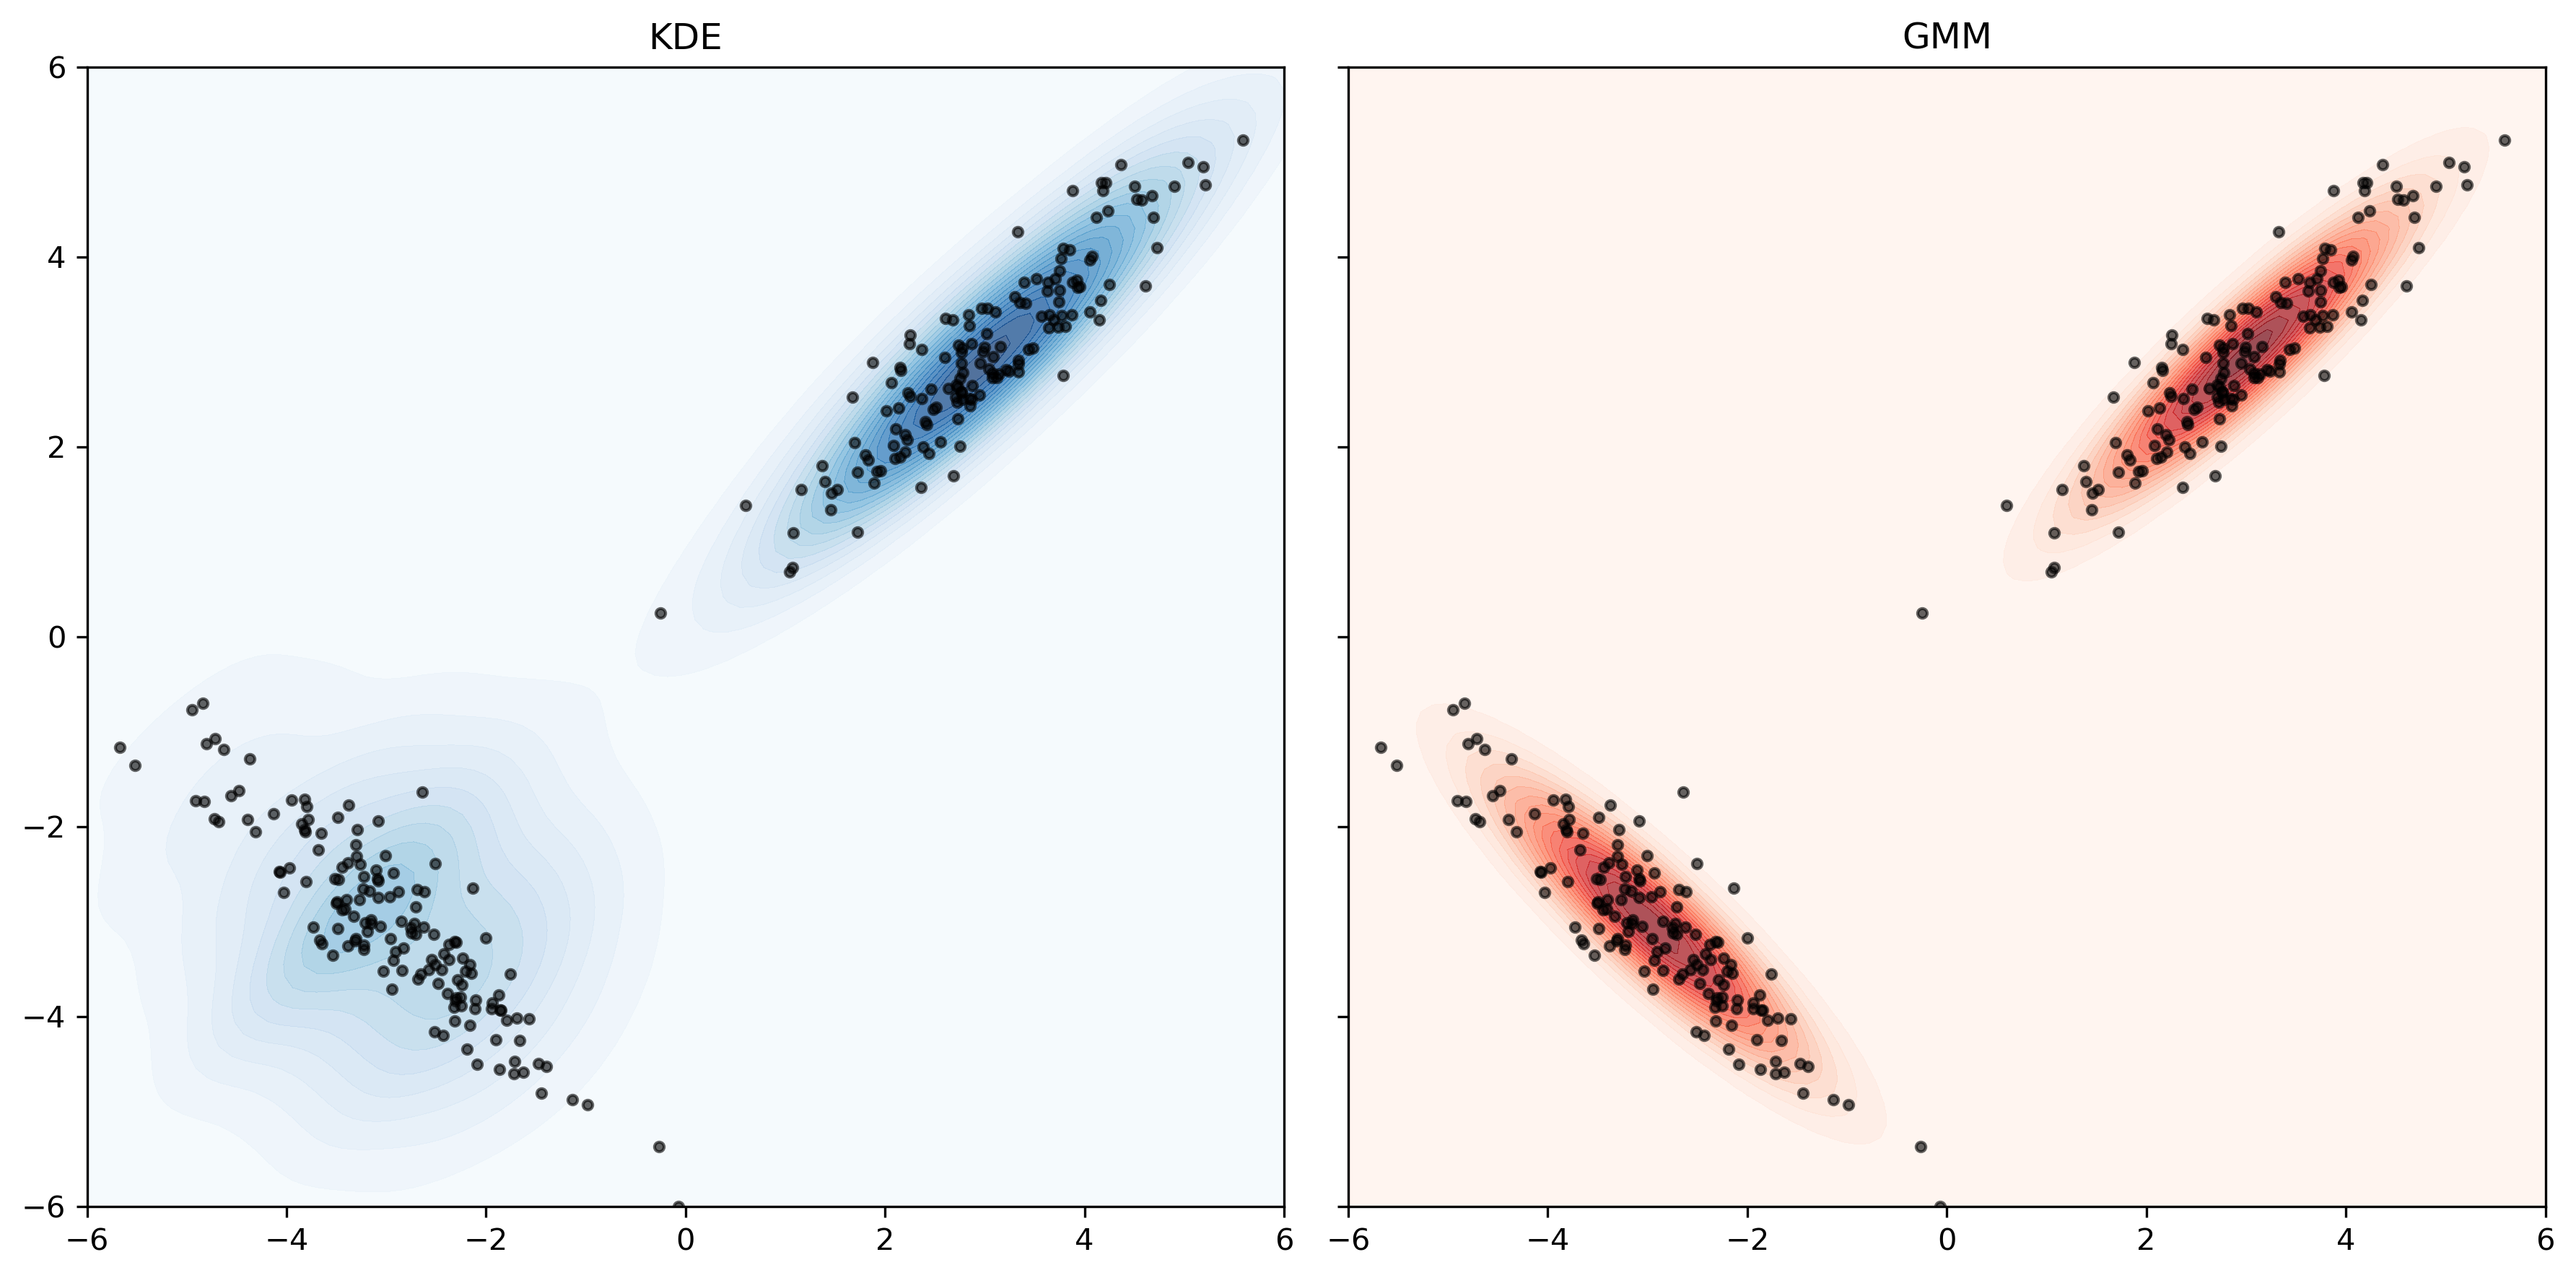
\includegraphics[width=\textwidth]{images/20_2.png}
  \caption[Best case scenario - GMM]{A two-component GMM more accurately recovers two correlated clusters than KDE. KDE (left, blue) and GMM densities (right, red; 2 components) for 300 samples drawn from two bivariate normals (150 points each) with strong negative and positive correlations. Colored filled contours show the estimated density; black dots are the data.}
  \label{fig:10_3}
\end{figure}

Both KDE and GMM describe the two-cluster structure (\ref{fig:10_3}) well, but GMM does so with only $K$=2 components, against KDE's $n$=300 kernels. When data exhibit clear Gaussian clusters, GMM is far more parsimonious; however, such distinct multimodality rarely occurs in financial returns. There is a tradeoff between GMM's parametric efficiency and KDE's nonparametric flexibility. GMM components remain strictly elliptical by construction, whereas KDE contours adapt to local data shape.

The parsimony of GMM can become a limitation when the data structure is highly nonlinear. In the following example, we present a noisy circular distribution that illustrates this, again drawing 300 observations. Each point's radial distance from the origin follows a normal distribution centered at $3$ with a standard deviation of $0.3$, while the angular positions are uniformly distributed over $[0, 2\pi]$:
$$\displaystyle (\begin{smallmatrix} x_1 \\ x_2 \end{smallmatrix}) = \left(3 + \epsilon\right) (\begin{smallmatrix} \cos\theta \\ \sin\theta \end{smallmatrix}), \quad \theta \sim \text{Uniform}(0, 2\pi), \quad \epsilon \sim \mathcal{N}(0, 0.3^2)$$

\begin{figure}[H]
  \centering
  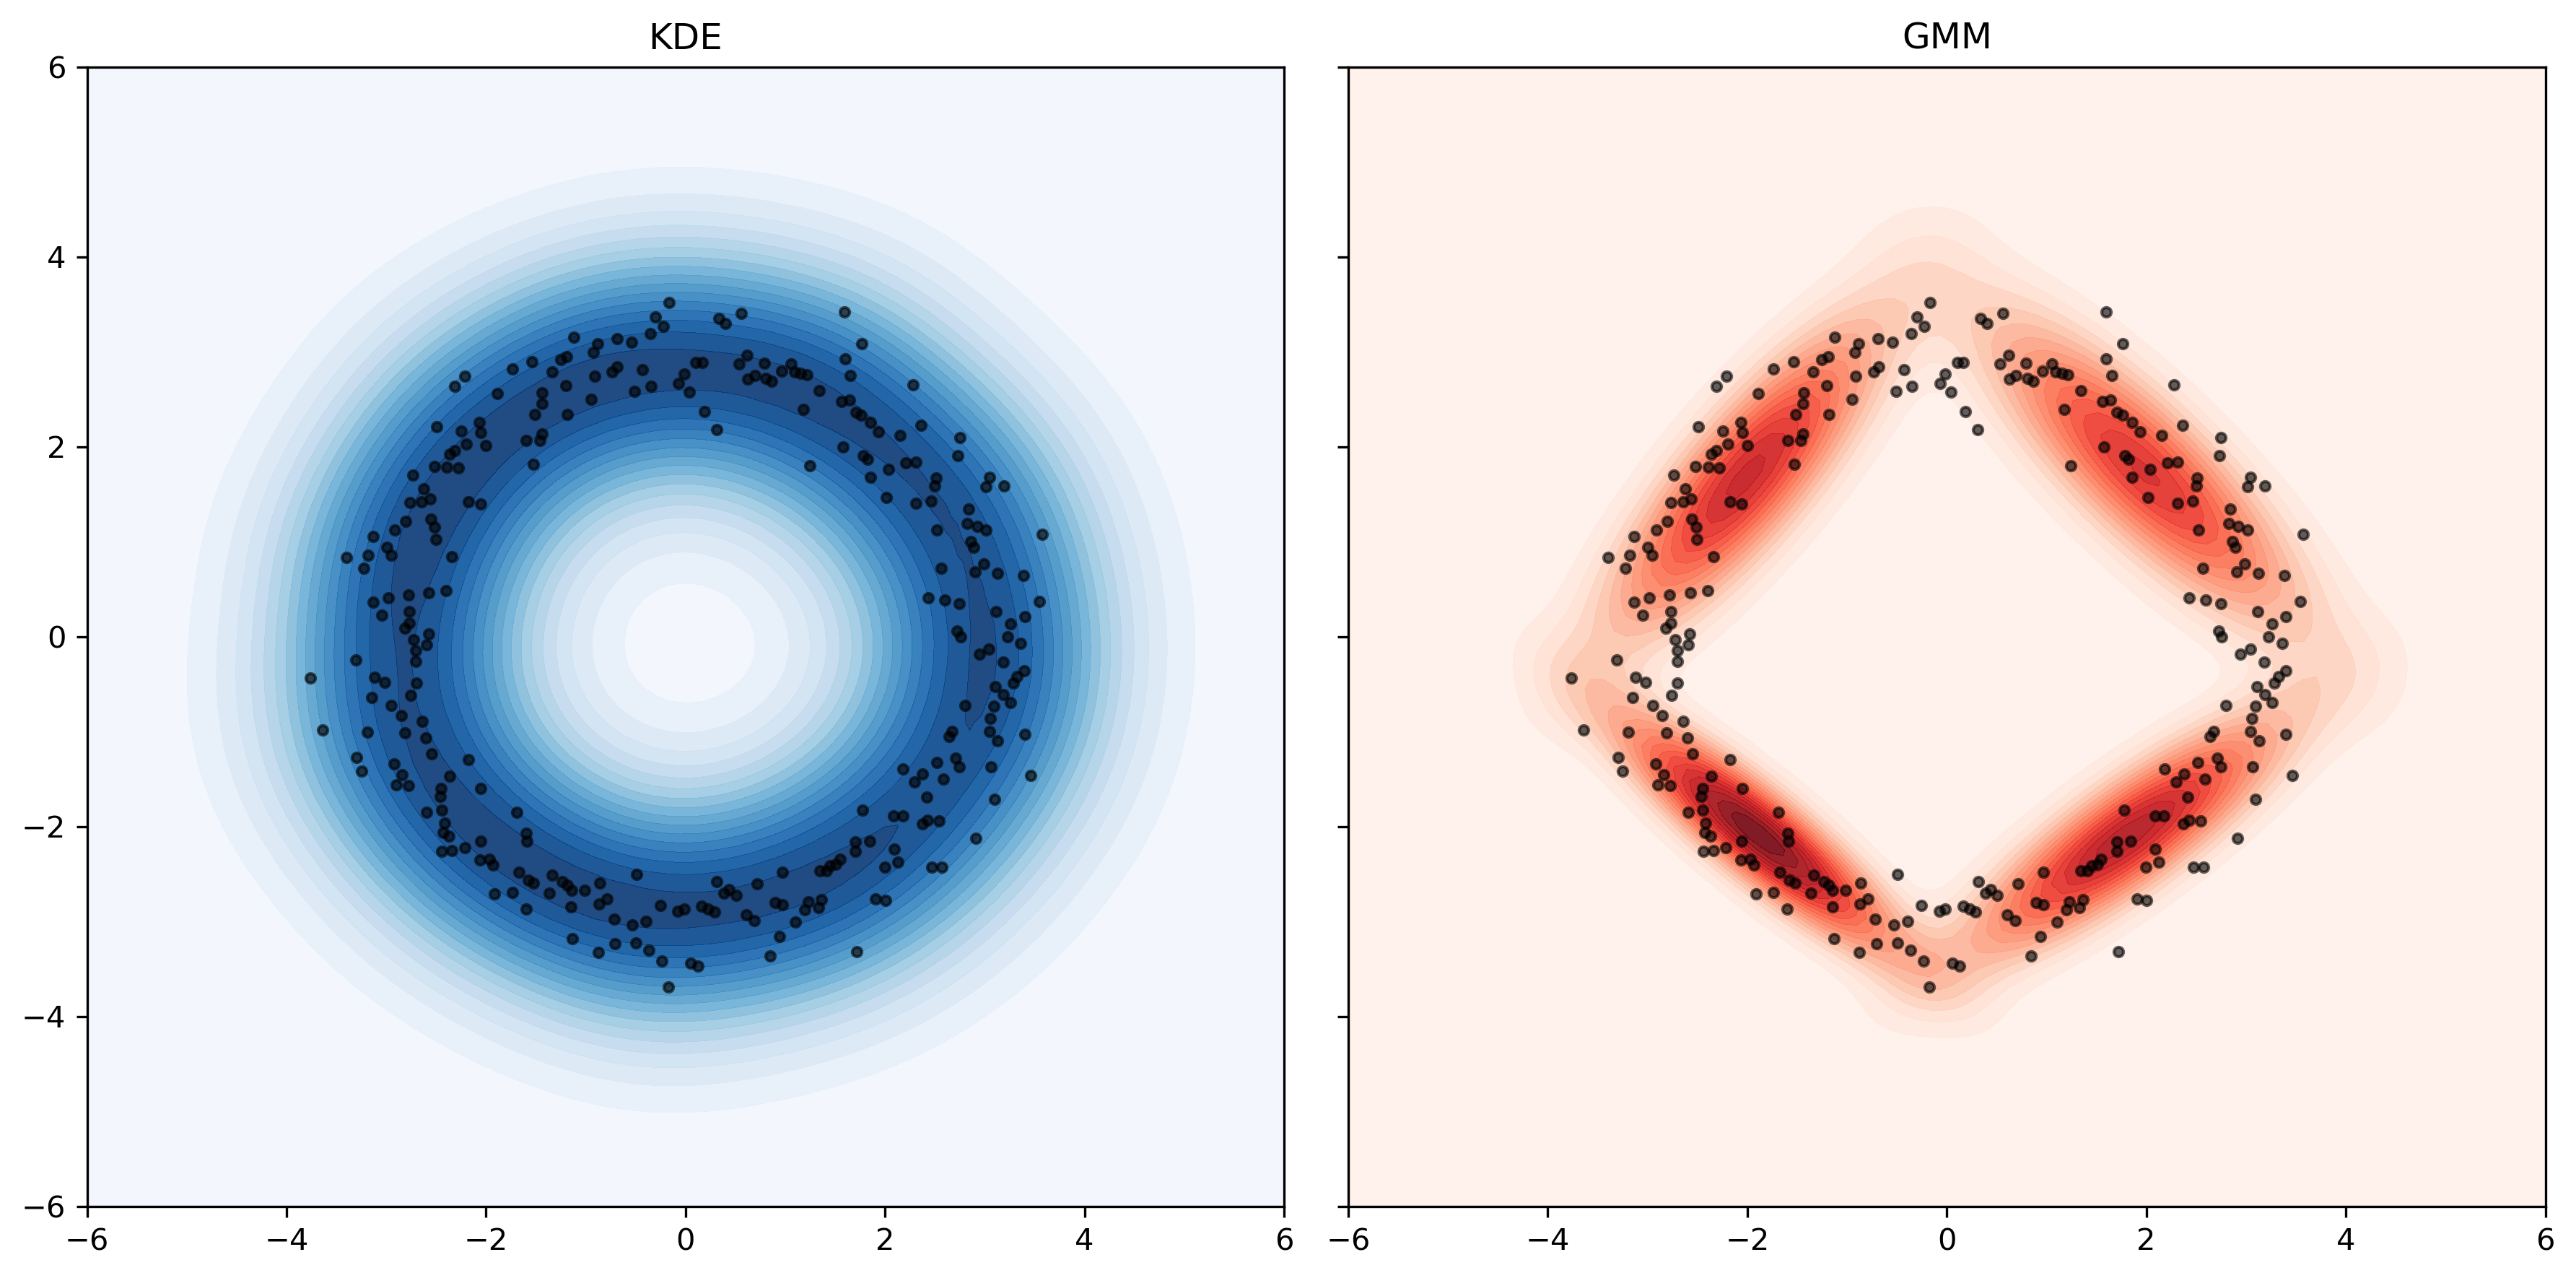
\includegraphics[width=\textwidth]{images/20_3.png}
  \caption[Best case scenario - KDE]{KDE captures a continuous ring-shaped density that GMM decomposes into discrete blobs. KDE (left, blue) and GMM (right, red; 4 components) for 300 points sampled around a noisy circle of radius $\approxeq$3. Colored filled contours show the estimated density; black dots are the data. }
  \label{fig:10_4}
\end{figure}

In this example, we used $K=4$ GMM components, which is evidently insufficient to describe the circular distribution. Increasing $K$ would reduce this bias, but at the cost of greater computational complexity. Therefore, when modeling data that exhibits nonlinear dependence structures, KDE's flexibility may outweigh GMM's theoretical efficiency.

In the context of our portfolio optimization framework (Chapter~\ref{chap:portfolio}), the use of a KDE density is usually significantly faster than GMM, especially as the window size grows large. The pitfall of GMM is the model estimation step, which quickly overshadows the higher cost of KDE at the optimization step. Inquisitive readers may refer to Appendix \ref{app:compute} for more on computational aspects.

\subsection{Log-Sum-Exponent and Softmax}
In Chapter~\ref{chap:portfolio}, we will encounter the log-sum-exponent (LSE) operator as the key building block of our portfolio objective. To prepare, we introduce it here and summarize its main properties. The complete derivation of its gradient and Hessian is given in Appendix~\ref{app:lse}.

Let $f(\mathbf{w})=(f_1(\mathbf{w}), f_2(\mathbf{w}),...,f_k(\mathbf{w}))^{\mathsf{T}}$ be a vector valued, twice-differentiable function. The log-sum-exponent operator of $f$ is defined as:
$$LSE_i(f_i(\mathbf{w}))=\log{\sum_{i=1}^{k}\exp(f_i(\mathbf{w}))}$$

Associated with LSE is the softmax function, which produces a probability distribution over the indices $i=1,...,k$:
$$\mathrm{softmax}_i(f)=p_i=\frac{{\exp( f_i(\mathbf{w}))}}{\sum_{i=1}^{k}\exp (f_i(\mathbf{w}))}$$
Softmax acts as a smooth approximation to the max operator, in that it concentrates weight on the largest components (\cite{boydConvexOptimization2004}).

$\textbf{Gradient of LSE}$: 
\newline
Define
$$S=\sum_{i=1}^k \exp{f_i(\mathbf w)}.$$
Then
$$\nabla_\mathbf w\,\mathrm{LSE}(f) = \nabla_\mathbf w\log S = \frac{1}{S}\,\nabla_\mathbf w S = \sum_{i=1}^k p_i\,\nabla f_i(\mathbf w).$$
In other words, the gradient of LSE is the softmax-weighted average of the individual gradients $\nabla f_i$.

$\textbf{Hessian of LSE}$: 
\newline
The Hessian matrix $\nabla^2 \mathrm{LSE}(f)$ can be expressed in terms of the component Hessians and gradients:
$$\nabla^2 \mathrm{LSE}(f) = \sum_{i=1}^k p_i \bigl[\nabla^2 f_i + (\nabla f_i)(\nabla f_i)^{\mathsf{T}}\bigr] \cdot \Bigl(\sum_{i=1}^k p_i\,\nabla f_i\Bigr)\Bigl(\sum_{j=1}^k p_j\,\nabla f_j\Bigr)^{\mathsf{T}}$$
One can show (Appendix~\ref{app:lse}) that so long as $f(\mathbf{w})$ is convex, this matrix is positive semidefinite and therefore convex.

\chapter{Portfolio Construction}
\label{chap:portfolio}
\lhead{Chapter 3. \emph{Portfolio Construction}}

In the introduction, we discussed how relaxing the Gaussian assumption often sacrifices analytical clarity or leads to intractable estimation. By contrast, our GMM and KDE frameworks can capture skewness and heavy tails without giving up closed-form interpretability. This chapter builds on the classical mean-variance paradigm by combining our density estimators with exponential utility maximization. The resultant portfolios incorporate information about higher moments of asset returns yet retain the tractability of Markowitz's original approach.

\section{Modeling Returns}
Let $\mathbf{r}$ represent a random vector of asset returns in $\mathbb{R}^{d}$, where $d$ is the number of assets. We observe a time series of $n$ return realizations, denoted as
$$\mathbf{r}_{1},\mathbf{r}_2,...,\mathbf{r}_{n}\quad\text{where}\quad \mathbf{r}_{\it{i}}\in\mathbb{R}^{d}.$$

The portfolio return is defined as the scalar random variable
$$R(\mathbf{w})=\mathbf{w}^{\mathsf{T}}\mathbf{r},$$
where $\mathbf{w}\in\mathbb{R}^{d}$ is the vector of portfolio weights. Under exponential utility, the investor has the utility function
$$U(R(\mathbf{w}))=-\exp(-\gamma\mathbf{w}^{\mathsf{T}}\mathbf{r}),$$
with $\gamma$ is the risk aversion parameter.

Both KDE and GMM estimate the density of $\mathbf{r}\rightarrow\hat{f}(\mathbf{r})$, enabling us to compute the expected utility of the portfolio return:
$$\mathbb{E}[U(R(\mathbf{w}))]=\int_{\mathbb{R}^{d}}-\exp(-\gamma\mathbf{w}^{\mathsf{T}}\mathbf{r})\cdot\hat{f}(\mathbf{r})\,d\mathbf{r}$$

Since both KDE and GMM approximate the density as a weighted sum of Gaussian components, 
we can compute the overall expected utility as the weighted sum of expectations over each density component.

Now we recall the KD estimator: 
$$\displaystyle\hat{f_h}(\mathbf{x})=\frac{1}{n}\sum_{i=1}^{n}K_\mathbf{H}(\mathbf{x}-\mathbf{x}_i),$$
for which when Gaussian kernel is used, $K_\mathbf{H}$ can be written as
$$K_\mathbf{H}(\mathbf{r}-\mathbf{r}_i)=\mathcal{N}(\mathbf{r|r_{\it{i}},H}).$$

Additionally, we recall the known result for Gaussian expectations:
$$\mathbb{E}_{\mathbf{r}\sim\mathcal{N}(\mathbf{\mu,\Sigma})}[\exp(-\gamma\mathbf{w}^{\mathsf{T}}\mathbf{r})]=\exp\left(-\gamma\mathbf{w}^{\mathsf{T}}\mathbf{\mu}+\frac{1}{2}\gamma^2\mathbf{w}^{\mathsf{T}}\mathbf{\Sigma}\mathbf{w}\right)$$

Having established the above, we take the expectation under GMM and KDE side by side to demonstrate their similarity:
$$GMM:\qquad\mathbb{E}[U(R(\mathbf{w}))]=\int_{\mathbb{R}^{d}}-\exp(-\gamma\mathbf{w}^{\mathsf{T}}\mathbf{r})\cdot\sum_{i=1}^{K}\phi_{i} \mathcal{N}(\mathbf{r|\mu_{\it{i}},\Sigma_{\it{i}}})\,d\mathbf{r}$$

$$\,KDE:\qquad\mathbb{E}[U(R(\mathbf{w}))]=\int_{\mathbb{R}^{d}}-\exp(-\gamma\mathbf{w}^{\mathsf{T}}\mathbf{r})\cdot \sum_{i=1}^{n}\frac{1}{n}\mathcal{N}(\mathbf{r|r_{\it{i}},H})\,d\mathbf{r}\,$$

Which, by linearity, is equivalent to:
$$GMM:\qquad=-\sum_{i=1}^{K}\phi_{i}\int_{\mathbb{R}^{d}}\exp(-\gamma\mathbf{w}^{\mathsf{T}}\mathbf{r})\cdot \mathcal{N}(\mathbf{r|\mu_{\it{i}},\Sigma_{\it{i}}})\,d\mathbf{r}$$

$$\,KDE:\qquad=-\frac{1}{n}\sum_{i=1}^{n}\int_{\mathbb{R}^{d}}\exp(-\gamma\mathbf{w}^{\mathsf{T}}\mathbf{r})\cdot \mathcal{N}(\mathbf{r|r_{\it{i}},H})\,d\mathbf{r}\,\,\,$$

Substituting the normal density:
$$GMM:\qquad=-\sum_{i=1}^{K}\phi_{i}\int_{\mathbb{R}^{d}}\exp(-\gamma\mathbf{w}^{\mathsf{T}}\mathbf{r})\cdot \frac{1}{(2\pi)^{d/2}\sqrt{\det{(\mathbf{\Sigma_{\it{i}}})}}}\exp\left(-\frac{1}{2}\mathbf{(r-\mu_{\it{i}})^\mathsf{T}\Sigma_{\it{i}}^\mathrm{-1}(r-\mu_{\it{i}})}\right)d\mathbf{r}\,$$

$$\,KDE:\qquad\displaystyle=-\frac{1}{n}\sum_{i=1}^{n}\int_{\mathbb{R}^{d}}\exp(-\gamma\mathbf{w}^{\mathsf{T}}\mathbf{r})\cdot\frac{1}{(2\pi)^{d/2}\sqrt{\det{(\mathbf{H})}}}\exp\left(-\frac{1}{2}\mathbf{(r-r_{\it{i}})^\mathsf{T}H^\mathrm{-1}(r-r_{\it{i}})}\right)d\mathbf{r}\,$$

Finally, by applying the Gaussian expectation, we obtain:
$$GMM:\qquad\mathbb{E}[U(R(\mathbf{w}))]=-\sum_{i=1}^{K}\phi_{i}\exp\left(-\gamma\mathbf{w}^{\mathsf{T}}\mathbf{\mu}_i+\frac{1}{2}\gamma^2\mathbf{w}^{\mathsf{T}}\mathbf{\Sigma}_i\mathbf{w}\right)$$

$$\qquad\quad\equiv-\sum_{i=1}^{K}\phi_{i}\mathbb{E}_{i}[U(R(\mathbf{w}))]$$

Where $\mathbb{E}_{i}[U(R(\mathbf{w}))]$ is the expected utility for each of the $K$ Gaussian kernels.
$$\,KDE:\qquad\mathbb{E}[U(R(\mathbf{w}))]=-\frac{1}{n}\sum_{i=1}^{n}\exp\left(-\gamma\mathbf{w}^{\mathsf{T}}\mathbf{r}_i+\frac{1}{2}\gamma^2\mathbf{w}^{\mathsf{T}}\mathbf{H}\mathbf{w}\right)$$
$$\qquad\qquad\qquad\qquad\qquad\qquad\,\,=-\frac{1}{n}\exp\left(\frac{1}{2}\gamma^2\mathbf{w}^{\mathsf{T}}\mathbf{H}\mathbf{w}\right)\sum_{i=1}^{n}\exp\left(-\gamma\mathbf{w}^{\mathsf{T}}\mathbf{r}_i\right)$$


\section{Portfolio Construction}
\subsection{GMM Portfolio}
Having derived exact expressions for $\mathbb{E}[U(R(\mathbf w))]$ under each return model, all that is left is the choice of the optimal $\mathbf w$. We begin by maximizing the expected utility:

\begin{align*}
\arg\max_\mathbf{w}{\mathbb{E}[U(R(\mathbf{w}))]} &= \arg\max_\mathbf{w}{-\sum_{i=1}^{K}\phi_{i}\exp\left(-\gamma\mathbf{w}^{\mathsf{T}}\mathbf{\mu}_i+\frac{1}{2}\gamma^2\mathbf{w}^{\mathsf{T}}\mathbf{\Sigma}_i\mathbf{w}\right)} \\
\intertext{Since multiplying by -1 flips the maximization into minimization, we rewrite the objective as}
&= \arg\min_\mathbf{w}{\sum_{i=1}^{K}\phi_{i}\exp\left(-\gamma\mathbf{w}^{\mathsf{T}}\mathbf{\mu}_i+\frac{1}{2}\gamma^2\mathbf{w}^{\mathsf{T}}\mathbf{\Sigma}_i\mathbf{w}\right)} \\
\intertext{To simplify the exponential sum and exploit convexity, we apply the monotonic logarithm, yielding}
&= \arg\min_\mathbf{w}\log{\left[{\sum_{i=1}^{K}\phi_{i}\exp\left(-\gamma\mathbf{w}^{\mathsf{T}}\mathbf{\mu}_i+\frac{1}{2}\gamma^2\mathbf{w}^{\mathsf{T}}\mathbf{\Sigma}_i\mathbf{w}\right)}\right]} \\
\intertext{Factoring out the component weights inside the exponent gives}
&= \arg\min_\mathbf{w}\log{\left[{\sum_{i=1}^{K}\exp({\log{\phi_{i}}})\exp\left(-\gamma\mathbf{w}^{\mathsf{T}}\mathbf{\mu}_i+\frac{1}{2}\gamma^2\mathbf{w}^{\mathsf{T}}\mathbf{\Sigma}_i\mathbf{w}\right)}\right]} \\
&= \arg\min_\mathbf{w}\log{\left[{\sum_{i=1}^{K}\exp\left(\log{\phi_{i}}-\gamma\mathbf{w}^{\mathsf{T}}\mathbf{\mu}_i+\frac{1}{2}\gamma^2\mathbf{w}^{\mathsf{T}}\mathbf{\Sigma}_i\mathbf{w}\right)}\right]} \\
\intertext{Recognizing this as the log-sum-exp operator (LSE), we obtain the compact form}
&= \arg\min_\mathbf{w}LSE_i\left(\log{\phi_{i}}-\gamma\mathbf{w}^{\mathsf{T}}\mathbf{\mu}_i+\frac{1}{2}\gamma^2\mathbf{w}^{\mathsf{T}}\mathbf{\Sigma}_i\mathbf{w}\right)
\end{align*}

% Having derived exact expressions for $\mathbb{E}[U(R(\mathbf w))]$ under each return model, all that is left is the choice of the optimal $\mathbf w$. We begin by maximizing the expected utility:
% $$\arg\max_\mathbf{w}{\mathbb{E}[U(R(\mathbf{w}))]}=\arg\max_\mathbf{w}{-\sum_{i=1}^{K}\phi_{i}\exp\left(-\gamma\mathbf{w}^{\mathsf{T}}\mathbf{\mu}_i+\frac{1}{2}\gamma^2\mathbf{w}^{\mathsf{T}}\mathbf{\Sigma}_i\mathbf{w}\right)}$$

% Since multiplying by -1 flips the maximization into minimization, we rewrite the objective as
% $$=\arg\min_\mathbf{w}{\sum_{i=1}^{K}\phi_{i}\exp\left(-\gamma\mathbf{w}^{\mathsf{T}}\mathbf{\mu}_i+\frac{1}{2}\gamma^2\mathbf{w}^{\mathsf{T}}\mathbf{\Sigma}_i\mathbf{w}\right)}$$

% To simplify the exponential sum and exploit convexity, we apply the monotonic logarithm, yielding
% $$=\arg\min_\mathbf{w}\log{\left[{\sum_{i=1}^{K}\phi_{i}\exp\left(-\gamma\mathbf{w}^{\mathsf{T}}\mathbf{\mu}_i+\frac{1}{2}\gamma^2\mathbf{w}^{\mathsf{T}}\mathbf{\Sigma}_i\mathbf{w}\right)}\right]}$$

% Factoring out the component weights inside the exponent gives
% $$=\arg\min_\mathbf{w}\log{\left[{\sum_{i=1}^{K}\exp({\log{\phi_{i}}})\exp\left(-\gamma\mathbf{w}^{\mathsf{T}}\mathbf{\mu}_i+\frac{1}{2}\gamma^2\mathbf{w}^{\mathsf{T}}\mathbf{\Sigma}_i\mathbf{w}\right)}\right]}$$

% $$=\arg\min_\mathbf{w}\log{\left[{\sum_{i=1}^{K}\exp\left(\log{\phi_{i}}-\gamma\mathbf{w}^{\mathsf{T}}\mathbf{\mu}_i+\frac{1}{2}\gamma^2\mathbf{w}^{\mathsf{T}}\mathbf{\Sigma}_i\mathbf{w}\right)}\right]}$$

% Recognizing this as the log-sum-exp operator (LSE), we obtain the compact form
% $$=\arg\min_\mathbf{w}LSE_i\left(\log{\phi_{i}}-\gamma\mathbf{w}^{\mathsf{T}}\mathbf{\mu}_i+\frac{1}{2}\gamma^2\mathbf{w}^{\mathsf{T}}\mathbf{\Sigma}_i\mathbf{w}\right)$$

Setting up Lagrangian and imposing the fully invested constraint:
$$\mathcal{L}=LSE_i\left(\log{\phi_{i}}-\gamma\mathbf{w}^{\mathsf{T}}\mathbf{\mu}_i+\frac{1}{2}\gamma^2\mathbf{w}^{\mathsf{T}}\mathbf{\Sigma}_i\mathbf{w}\right)+\lambda(\mathbf{w^{\mathsf{T}}1}-1)$$

For notational simplicity, let us define
$$f_i(\mathbf{w})=\log{\phi_{i}}-\gamma\mathbf{w}^{\mathsf{T}}\mathbf{\mu}_i+\frac{1}{2}\gamma^2\mathbf{w}^{\mathsf{T}}\mathbf{\Sigma}_i\mathbf{w}$$
$$\Longrightarrow \mathcal{L}=LSE_i(f_i(\mathbf{w}))-\lambda(\mathbf{w^{\mathsf{T}}1})$$

Differentiating the Lagrangian with respect to $\mathbf w$ gives
$$\frac{\partial\mathcal{L}}{\partial\mathbf{w}}=\frac{\partial}{\partial\mathbf{w}}LSE_i(f_i(\mathbf{w}))+\lambda\mathbf{1}$$

By the result in Chapter~\ref{chap:math}, the LSE gradient is
$$
\nabla_{\mathbf w}\mathrm{LSE}(f)
= \sum_{i=1}^K p_i\nabla f_i(\mathbf w),
\quad
p_i = \frac{\exp\bigl(f_i(\mathbf w)\bigr)}{\sum_{j=1}^K\exp\bigl(f_j(\mathbf w)\bigr)}.
$$

Recalling the function $f_i(\mathbf{w})$ and taking its derivative
$$\frac{\partial}{\partial\mathbf{w}}f_i(\mathbf{w})=-\gamma\mathbf{\mu}_i+\gamma^2\mathbf{\Sigma}_i\mathbf{w}$$

Allows us to complete the LSE derivative and write the FOC of the Lagrangian as
\begin{align*}
  \frac{\partial\mathcal{L}}{\partial\mathbf{w}}:\quad\sum_{i=1}^{K}p_i(-\gamma\mathbf{\mu}_i+\gamma^2\mathbf{\Sigma}_i\mathbf{w})+\lambda\mathbf{1}=&\;0 \\
  \gamma^2\sum_{i=1}^{K}p_i\mathbf{\Sigma}_i\mathbf{w}-\gamma\sum_{i=1}^{K}p_i\mathbf{\mu}_i+\lambda\mathbf{1}=&\;0
\end{align*} 

For notational brevity, let
$$A\equiv\sum_{i=1}^{K}p_i\mathbf{\Sigma}_{i}\qquad b\equiv\sum_{i=1}^{K}p_i\mathbf{\mu}_i$$
$$\Longrightarrow \gamma^{2}A\mathbf{w}-\gamma b\mathbf{\mu}_{i}+\lambda\mathbf{1}=0$$
$$\mathbf{w}=\frac{1}{\gamma}A^{-1}(b-\frac{\lambda}{\gamma}\mathbf{1})$$

After which we impose the budget constraint $\mathbf{w^{\mathsf{T}}1}=1$ and deduce the optimal Lagrange multiplier
$$1=\frac{1}{\gamma}\mathbf{1}^{\mathsf{T}}A^{-1}b-\frac{\lambda}{\gamma^2}\mathbf{1}^{\mathsf{T}}A^{-1}\mathbf{1}$$
$$-\frac{\lambda}{\gamma^2}=\frac{1-\frac{1}{\gamma}\mathbf1^T A^{-1}b} {\mathbf1^T A^{-1}\mathbf1}$$

Allowing us to finally obtain the form of the optimal solution
$$\Longrightarrow\mathbf{w}^* = \frac{1}{\gamma} A^{-1} b + \left(\frac{1-\frac{1}{\gamma}\mathbf1^T A^{-1}b} {\mathbf1^T A^{-1}\mathbf1}\right) A^{-1} \mathbf{1}$$
$$\boxed{\mathbf{w}^* = \frac{1}{\gamma} A^{-1} b + \left(\frac{1}{\mathbf{1}^{\mathsf{T}} A^{-1} \mathbf{1}}- \frac{1}{\gamma}\frac{\mathbf{1}^{\mathsf{T}} A^{-1} b}{ \mathbf{1}^{\mathsf{T}} A^{-1} \mathbf{1}}\right) A^{-1} \mathbf{1}}$$
with
$$A\equiv\sum_{i=1}^{K} \frac{\exp f_i(\mathbf{w})}{\sum_{j=1}^{K} \exp f_j(\mathbf{w})} \mathbf{\Sigma}_{i}\qquad b\equiv \sum_{i=1}^{K} \frac{\exp f_i(\mathbf{w})}{\sum_{j=1}^{K} \exp f_j(\mathbf{w})} \mathbf{\mu}_i$$

\subsubsection{Interpretation}
Since the softmax weighting function depends on $\mathbf{w}$, we do not obtain an analytical solution for the optimal weights. Nevertheless, there is an encouraging equivalence between our solution and the usual Markowitz result - their forms coincide exactly. In fact, $A$ and $b$ will be equivalent to the sample moments $\Sigma$ and $\mu$ if either: only a single GMM cluster is used ($K$=1), or $p_i$ is uniform for all $i$.

The key distinction lies in how the mean and covariance are estimated. Instead of using sample moments, our solution employs softmax-weighted estimators, which dynamically adjust the influence of each Gaussian component based on its expected utility. This weighting scheme ensures that scenarios associated with worse outcomes receive greater emphasis. 

To better understand this effect, we first recall that:
$$\text{Softmax}(f(\mathbf{w}))_i=p_i=\frac{{\exp f_i(\mathbf{w})}}{\sum_{i=1}^{K}\exp f_i(\mathbf{w})}$$
$$\mathbb{E}[U(R(\mathbf{w}))]=-\sum_{i=1}^{K}\phi_{i}\mathbb{E}_{i}[U(R(\mathbf{w}))]$$
$$f_i(\mathbf{w})=\log{\phi_{i}}-\gamma\mathbf{w}^{\mathsf{T}}\mathbf{\mu}_i+\frac{1}{2}\gamma^2\mathbf{w}^{\mathsf{T}}\mathbf{\Sigma}_i\mathbf{w}$$
Where $\mathbb{E}_{i}[U(R(\mathbf{w}))]$ is the expected utility for each of the $K$ Gaussian components:
$$-\mathbb{E}_{i}[U(R(\mathbf{w}))]=\exp\left(-\gamma\mathbf{w}^{\mathsf{T}}\mathbf{\mu}_i+\frac{1}{2}\gamma^2\mathbf{w}^{\mathsf{T}}\mathbf{\Sigma}_i\mathbf{w}\right)$$

Hence, we can rewrite $f_i(\mathbf{w})$ as:
$$f_i(\mathbf{w})=\log{(\phi_i)}+\log{(-\mathbb{E}_{i}[U(R(\mathbf{w}))])}$$
$$=\log{\{-\phi_i\,\mathbb{E}_{i}[U(R(\mathbf{w})]\}}\;\,\,$$
Which yields the following formulation for $p_i$:
$$p_i=\frac{{\exp \log{\{-\phi_i\,\mathbb{E}_{i}[U(R(\mathbf{w})]\}}}}{\sum_{i=1}^{K}\exp \log{\{-\phi_i\,\mathbb{E}_{i}[U(R(\mathbf{w})]\}}}$$
$$=\frac{{\phi_i\cdot\{-\mathbb{E}_{i}[U(R(\mathbf{w})]\}}}{\sum_{i=1}^{K}\phi_i\cdot\{-\mathbb{E}_{i}[U(R(\mathbf{w})]\}}$$

This should hopefully make it clear that the weighting factor $p_i$ is higher, the lower the expected utility is. Now recalling the definitions of $A$ and $b$:
$$A\equiv\sum_{i=1}^{K}p_i\mathbf{\Sigma}_{i}\qquad b\equiv\sum_{i=1}^{K}p_i\mathbf{\mu}_i$$

We see that $A$ and $b$ are simply the weighted average estimators of $\Sigma$ and $\mu$, respectively. With $p_i$ being inversely related to the expected utility of component $i$, these generalized estimators assign greater weight to those components of the Gaussian mixture that are expected to yield the least favorable outcomes. 

If one Gaussian component corresponds to a fat-tail crash scenario, its low utility will inflate $p_i$ and hence its covariance enters more heavily into $A$. This weighting mechanism naturally incorporates downside risk into the moment estimates instead of simply relying on sample moments that may understate the influence of adverse market conditions.




\subsection{Kernel Density Portfolio}
The KDE portfolio construction follows the same high-level recipe as the GMM case (see Appendix~\ref{app:kde} for the full derivation). We begin by maximizing the expected exponential utility under the KDE density:
$$\arg\max_\mathbf{w}{\mathbb{E}[U(R(\mathbf{w}))]}=\arg\max_\mathbf{w}{-\frac{1}{n}\exp\left(\frac{1}{2}\gamma^2\mathbf{w}^{\mathsf{T}}\mathbf{H}\mathbf{w}\right)\sum_{i=1}^{n}\exp\left(-\gamma\mathbf{w}^{\mathsf{T}}\mathbf{r}_i\right)}$$

Since neither the bandwidth matrix $H$ nor the normalization $1/n$ depend on $i$, the LSE term simplifies to aggregate the returns scaled by $\gamma$ and $\mathbf{w}$:
$$=\arg\min_\mathbf{w}\frac{1}{2}\gamma^2\mathbf{w}^{\mathsf{T}}\mathbf{H}\mathbf{w}+LSE(-\gamma\mathbf{w}^{\mathsf{T}}\mathbf{r}_i)-\log{n}$$

Since $-\log{n}$ is constant in $\mathbf{w}$, it does not affect the optimal solution and is dropped. We then set up the Lagrangian with a fully invested constraint:
$$\mathcal{L}=\frac{1}{2}\gamma^2\mathbf{w}^{\mathsf{T}}\mathbf{H}\mathbf{w}+LSE(-\gamma\mathbf{w}^{\mathsf{T}}\mathbf{r}_i)+\lambda(\mathbf{w^{\mathsf{T}}1}-1)$$

Defining
$$g_i(\mathbf w)=-\gamma\mathbf{w}^{\mathsf{T}}\mathbf{r}_{i},
\quad p_i=\frac{\exp\left(g_i(\mathbf w)\right)}{\sum_{j=1}^n\exp\left(g_j(\mathbf w)\right)},\quad
c=\sum_{i=1}^n p_i\,\mathbf{r}_i,$$
we take the derivative, giving us the FOC:
$$\frac{\partial\mathcal{L}}{\partial\mathbf{w}}:\quad\gamma^{2}\mathbf{H}\mathbf{w}-\gamma c+\lambda\mathbf{1}=0$$

Imposing the $\mathbf w^\top\mathbf1=1$ constraint and solving the system yields the optimal form:
$$\boxed{\mathbf{w}^*=\frac{1}{\gamma}\mathbf{H}^{-1}c+\left(\frac{1}{\mathbf1^T \mathbf{H}^{-1}\mathbf1}-\frac{1}{\gamma}\frac{\mathbf{1}^{\mathsf{T}}\mathbf{H}^{-1}c}{\mathbf1^T \mathbf{H}^{-1}\mathbf1}\right)\mathbf{H}^{-1}\mathbf{1}}$$
With the fully expanded weighting factor $c$:
$$c\equiv \sum_{i=1}^{n} \frac{\exp (-\gamma\mathbf{w}^{\mathsf{T}}\mathbf{r}_{i})}{\sum_{j=1}^{n} \exp (-\gamma\mathbf{w}^{\mathsf{T}}\mathbf{r}_{j})} \mathbf{r}_i$$

\subsubsection{Interpretation}
Analogously to the GMM case, the KDE-based solution coincides with the classical mean-variance formula. Though arriving at a solution that is identical to Markowitz would require setting $H$ to the sample covariance matrix $\Sigma$, which does not align with the logic of kernel density estimation. Further, all $p_i$ would have to be uniform so that the $c$ term could become the sample mean ($c=\sum_{i=1}^n p_i\,r_i =\frac1n\sum_{i=1}^n r_i$).

But the real power of KDE lies in the data-driven weights it assigns to each return realization:
$$p_i \;=\; \frac{\exp\!\left(-\gamma\mathbf{w}^{\mathsf{T}}\mathbf{r}_{i}\right)} {\sum_j \exp\!\left(-\gamma\mathbf{w}^{\mathsf{T}}\mathbf{r}_{i}\right)}.$$
These weights have two complementary interpretations:
\begin{enumerate}
\item $\textbf{Soft-max of scaled portfolio returns}$: The mapping $-\gamma\mathbf{w}^{\mathsf{T}}\mathbf{r}_{i}$ penalizes adverse outcomes; the soft-max then amplifies their influence relative to neutral observations.
\item $\textbf{Normalised negative utilities}$: Since $U(R_i)=-\exp(-\gamma\mathbf{w}^{\mathsf{T}}\mathbf{r}_{i})$, each weighting factor $p_i$ can be written as $p_i=-U(R_i)\bigl/\sum_j -U(R_j);$
Each data point is weighted in proportion to the disutility it inflicts on the total disutility of the portfolio.
\end{enumerate}

Consequently, the optimal weights in the KDE framework naturally respond to adverse scenarios implicitly identified through an integrated backtest. Historical drawdowns pull $c$ downward, directly injecting downside information into the objective function. Investors thus internalize skew and tail-risk without resorting to ad-hoc skewness parameters or exotic utility functions.

This dynamic notably differs from GMM, where the mixture weights $\phi$ are fixed ex-ante by the EM algorithm. Under GMM, once the clusters are estimated, each portfolio optimizes using the same predetermined set of component moments. KDE, in contrast, recomputes $p_i(\mathbf w)$ ex-post, effectively letting the data "vote" according to how each trial allocation would have fared historically.

The resulting optimization preserves the convex structure of the mean-variance problem (see \ref{sec:convexity}), while embedding tail-aversion through the self-weighted mean $c(\mathbf w)$. Thus, KDE offers an analytically tractable and fully non-parametric bridge between Markowitz's Gaussian ideal and the skewed, heavy-tailed reality of empirical returns.

\section{Convexity}
\label{sec:convexity}
We briefly examine the convexity of the KDE and GMM objective functions to determine whether the optimization can be tackled with convex numerical optimization. First, we recall the LSE Hessian:
$$\mathbf{H}_{LSE}=\sum_{i=1}^{k}p_i\cdot\left[\mathbf{H}_{f_i}+\mathbf{J}_{f_i}^{}\,\mathbf{J}_{f_i}^{\mathsf{T}}\right]-\left(\sum_{i=1}^{k}p_i\mathbf{J}_{f_i}\right)\left(\sum_{j=1}^{k}p_j\mathbf{J}_{f_i}\right)^{\mathsf{T}}$$
Where $\mathbf{J}_{f_i}$ and $\mathbf{H}_{f_i}$ are the Jacobian and Hessian matrix of function $f_i(\mathbf{w})$ respectively. And $p_i$ is the weight given by the softmax function to each of the $f_i(\mathbf{w})$ functions.

Focusing on the Jacobian components, we can see that we have an expression resembling that of a covariance matrix, which, given that the softmax probabilities are strictly positive and always sum to 1 (\cite{boydConvexOptimization2004}), we can express them as:
$$\rightarrow \sum_{i=1}^{k}p_i\cdot\mathbf{J}_{f_i}^{}\,\mathbf{J}_{f_i}^{\mathsf{T}}-\left(\sum_{i=1}^{k}p_i\mathbf{J}_{f_i}\right)\left(\sum_{j=1}^{k}p_j\mathbf{J}_{f_i}\right)^{\mathsf{T}}=\mathbb{E}_{p}[\mathbf{J}_{f_i}^{}\,\mathbf{J}_{f_i}^{\mathsf{T}}]-\mathbb{E}_{p}[\mathbf{J}_{f_i}^{}]\,\mathbb{E}_{p}[\mathbf{J}_{f_i}^{}]^{\mathsf{T}}$$
Which is simply the weighted covariance matrix of the gradient vectors $\mathbf{J}_{f_i}$, which we can denote $\hat\Sigma_{\mathbf{J}_{f}}$. Therefore, we have:
$$\mathbf{H}_{LSE}=\sum_{i=1}^{k}p_i\cdot\mathbf{H}_{f_i}+\hat\Sigma_{\mathbf{J}_{f}}$$

The sum of PSD matrices is also PSD. Since the covariance matrix is guaranteed to be PSD, it follows that the Hessian of the log-sum-exp function will also be PSD so long as the weighted expectation of the Hessian is PSD. Given that $p_i>0\,\forall i$, the weighted expectation is guaranteed to be PSD if each $\mathbf{H}_{f_i}$ is PSD (\cite{hornMatrixAnalysis2017}).

Recalling the two objective functions we defined for GMM and KDE, respectively:
$$GMM:f_i(\mathbf{w})=\log{\phi_{i}}-\gamma\mathbf{w}^{\mathsf{T}}\mathbf{\mu}_i+\frac{1}{2}\gamma^2\mathbf{w}^{\mathsf{T}}\mathbf{\Sigma}_i\mathbf{w}$$
$$KDE:f_i(\mathbf{w})=-\gamma\mathbf{w}^{\mathsf{T}}\mathbf{r}_i\qquad \qquad \qquad \qquad \quad $$

We can write the Hessian for GMM as:
$$GMM:\mathbf{H}_{f_i}=\gamma^{2}\Sigma_i$$
Which is guaranteed to be PSD, since each covariance matrix $\Sigma_i$ is PSD, and $\gamma^2>0$. And for KDE, we have:
$$KDE:\mathbf{H}_{f_i}=\mathbf{0}\quad\,$$
Which is also PSD since the eigenvalues of a zero matrix are all $0$.

It follows immediately that for both the KDE and GMM, their objective functions, as well as the Hessian of the log-sum-exponent function, are PSD, and therefore both problems are convex in $\mathbf{w}$.

\section{Tangency Portfolios}
\label{sec:tangency}
The KDE and GMM can also be used to construct tangency portfolios. Once we have the mean vector and covariance matrix from either density estimator, the tangency portfolio is obtained by maximizing the Sharpe ratio. If $r_f$ is the risk-free rate, we solve
$$
\max_{\mathbf w}
\frac{\mathbf w^{\mathsf{T}}(\mu - r_f\mathbf1)}
{\sqrt{\mathbf w^{\mathsf{T}}\Sigma\mathbf w}}
\quad\text{s.t.}\quad \mathbf w^{\mathsf{T}}\mathbf1=1.
$$

% In both cases, with a zero risk-free rate, the optimal weights admit the familiar closed-form solution:
% $$
% \mathbf w^*
% =\frac{\Sigma^{-1}(\mu - r_f\,\mathbf1)}
% {\mathbf1^{\mathsf{T}}\Sigma^{-1}(\mu - r_f\,\mathbf1)},
% $$
With the only difference being the estimators of $\mu$ and $\Sigma$:
\begin{itemize}
\item \textbf{GMM case}: $\mu=\sum_{i=1}^K\phi_i\,\mu_i,$ and $\Sigma=\sum_{i=1}^K\phi_i\bigl[\Sigma_i+(\mu_i-\mu)(\mu_i-\mu)^{\mathsf{T}}\bigr].$
\item \textbf{KDE case}: $\mu=\bar r,$ $\Sigma=H + S,$ where $S$ is the sample covariance of $\mathbf{r}$.
\end{itemize}

% \newpage
\section{Efficient Frontier Analysis}
\label{sec:frontier}
The closed-form weights derived above invite a classical efficient-frontier inspection. We will therefore plot multiple frontiers for a grid of risk-aversion parameters ($\gamma \in[5,100]$) using a subset of the data from our later experiments (16 assets).

Just to the side of the Markowitz efficient frontier is the KDE frontier. For low values of $\gamma$, the frontiers are closely aligned. Recalling the equation for the KDE expected variance (\ref{eq:kdevar}), we see that the KDE frontier is bound to be pushed deeper into the volatility axis unless the bandwidth matrix $H$ is zero, which is the first reason for the rightward shift of the KDE frontier. As risk aversion increases, however, the KDE frontier does not attain a minimum. Instead, both expected return and volatility start increasing. This creates a section on the KDE frontier that appears suboptimal in risk-return space compared to the point that would have provided the lowest volatility.

\vspace{5mm}
\begin{figure}[H]
    \begin{center}
    \begin{minipage}{0.65\textwidth}
      \centering
      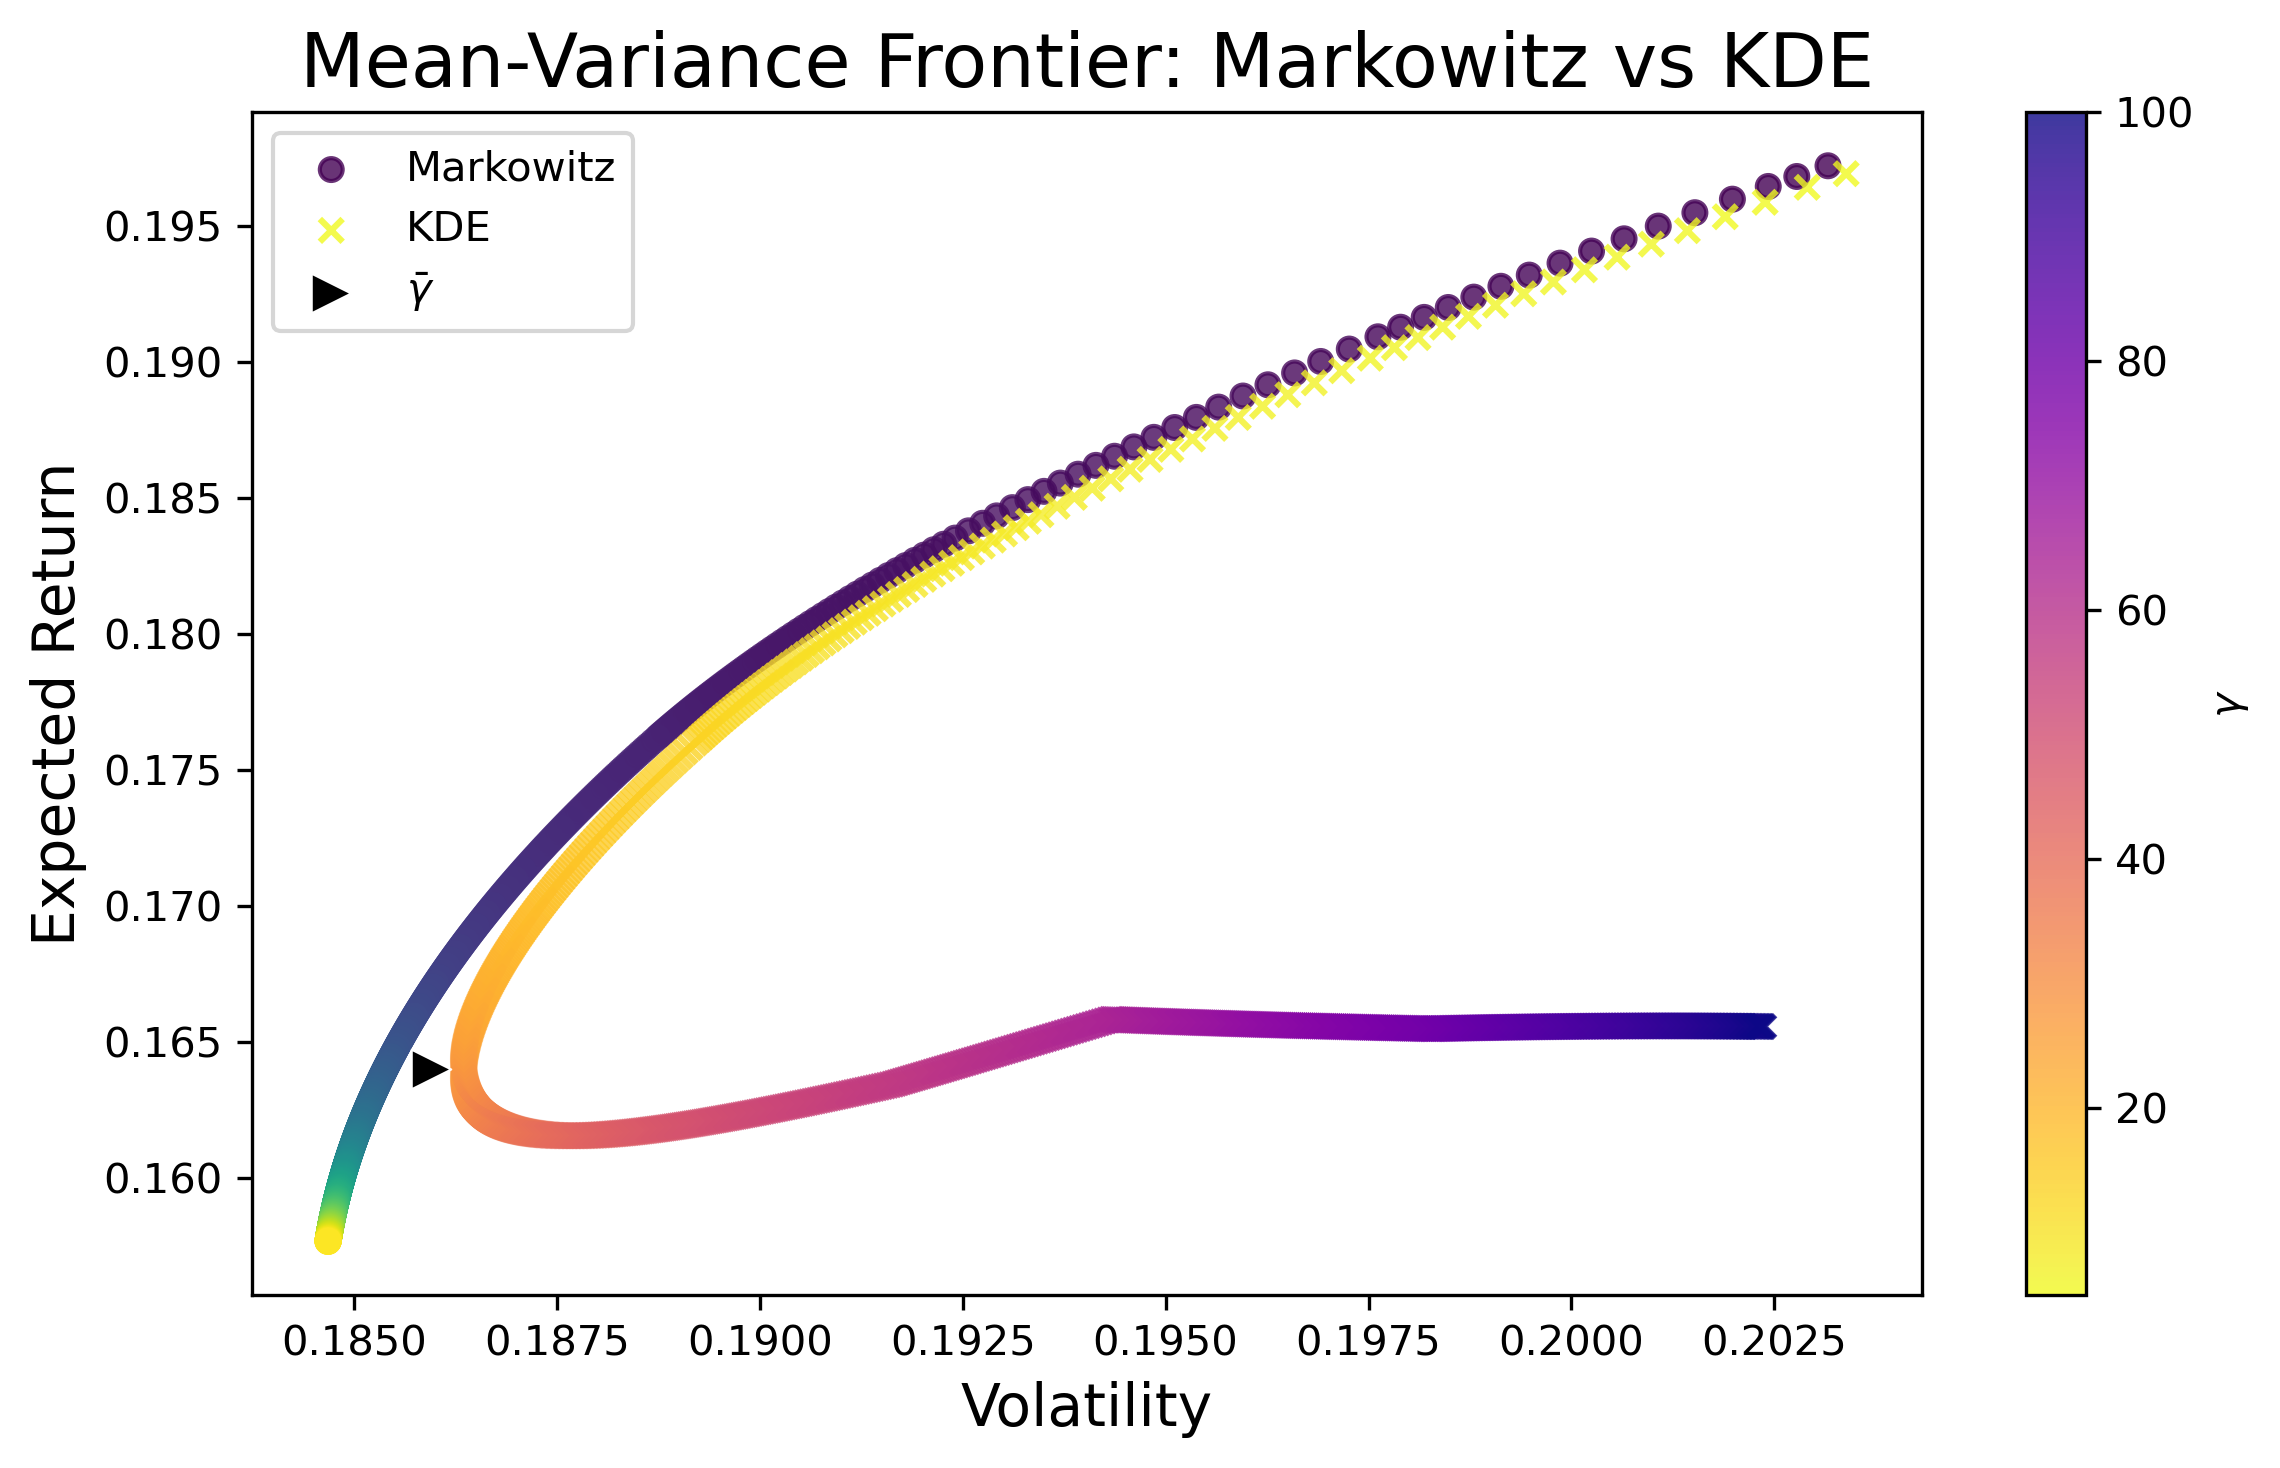
\includegraphics[width=\textwidth]{images/30_1.png}
    \end{minipage}
    \caption[Mean-variance frontier: Markowitz vs KDE]{Mean-variance efficient frontiers for risk-aversion parameters $\gamma\in[5,100]$, comparing classical Markowitz optimization (filled circles) with KDE-based optimization (crosses). Each marker is placed at the portfolio's expected volatility (x-axis) and expected return (y-axis) under a given $\gamma$, and colored from yellow (low risk aversion) to purple (high risk aversion). The $\blacktriangleright$ symbol indicates the minimum variance portfolio on the KDE frontier.}
    \label{fig:frontier1}
    \end{center}
    \end{figure}



This behavior contrasts with standard Markowitz optimization, where the highest risk aversion invariably results in the minimum variance portfolio. The KDE approach suggests a separation of two regimes of portfolio behavior, with a critical threshold value $\bar{\gamma}$. To better understand this phenomenon, we examine an alternative frontier situated in the risk-skewness space, rather than the risk-return space (using ex-post in-sample skewness). This second frontier shows that the apparent inefficiency in mean-variance space corresponds with improved skewness characteristics. 

\vspace{5mm}
\begin{figure}[H]
    \begin{center}
    \begin{minipage}{1\textwidth}
      \centering
      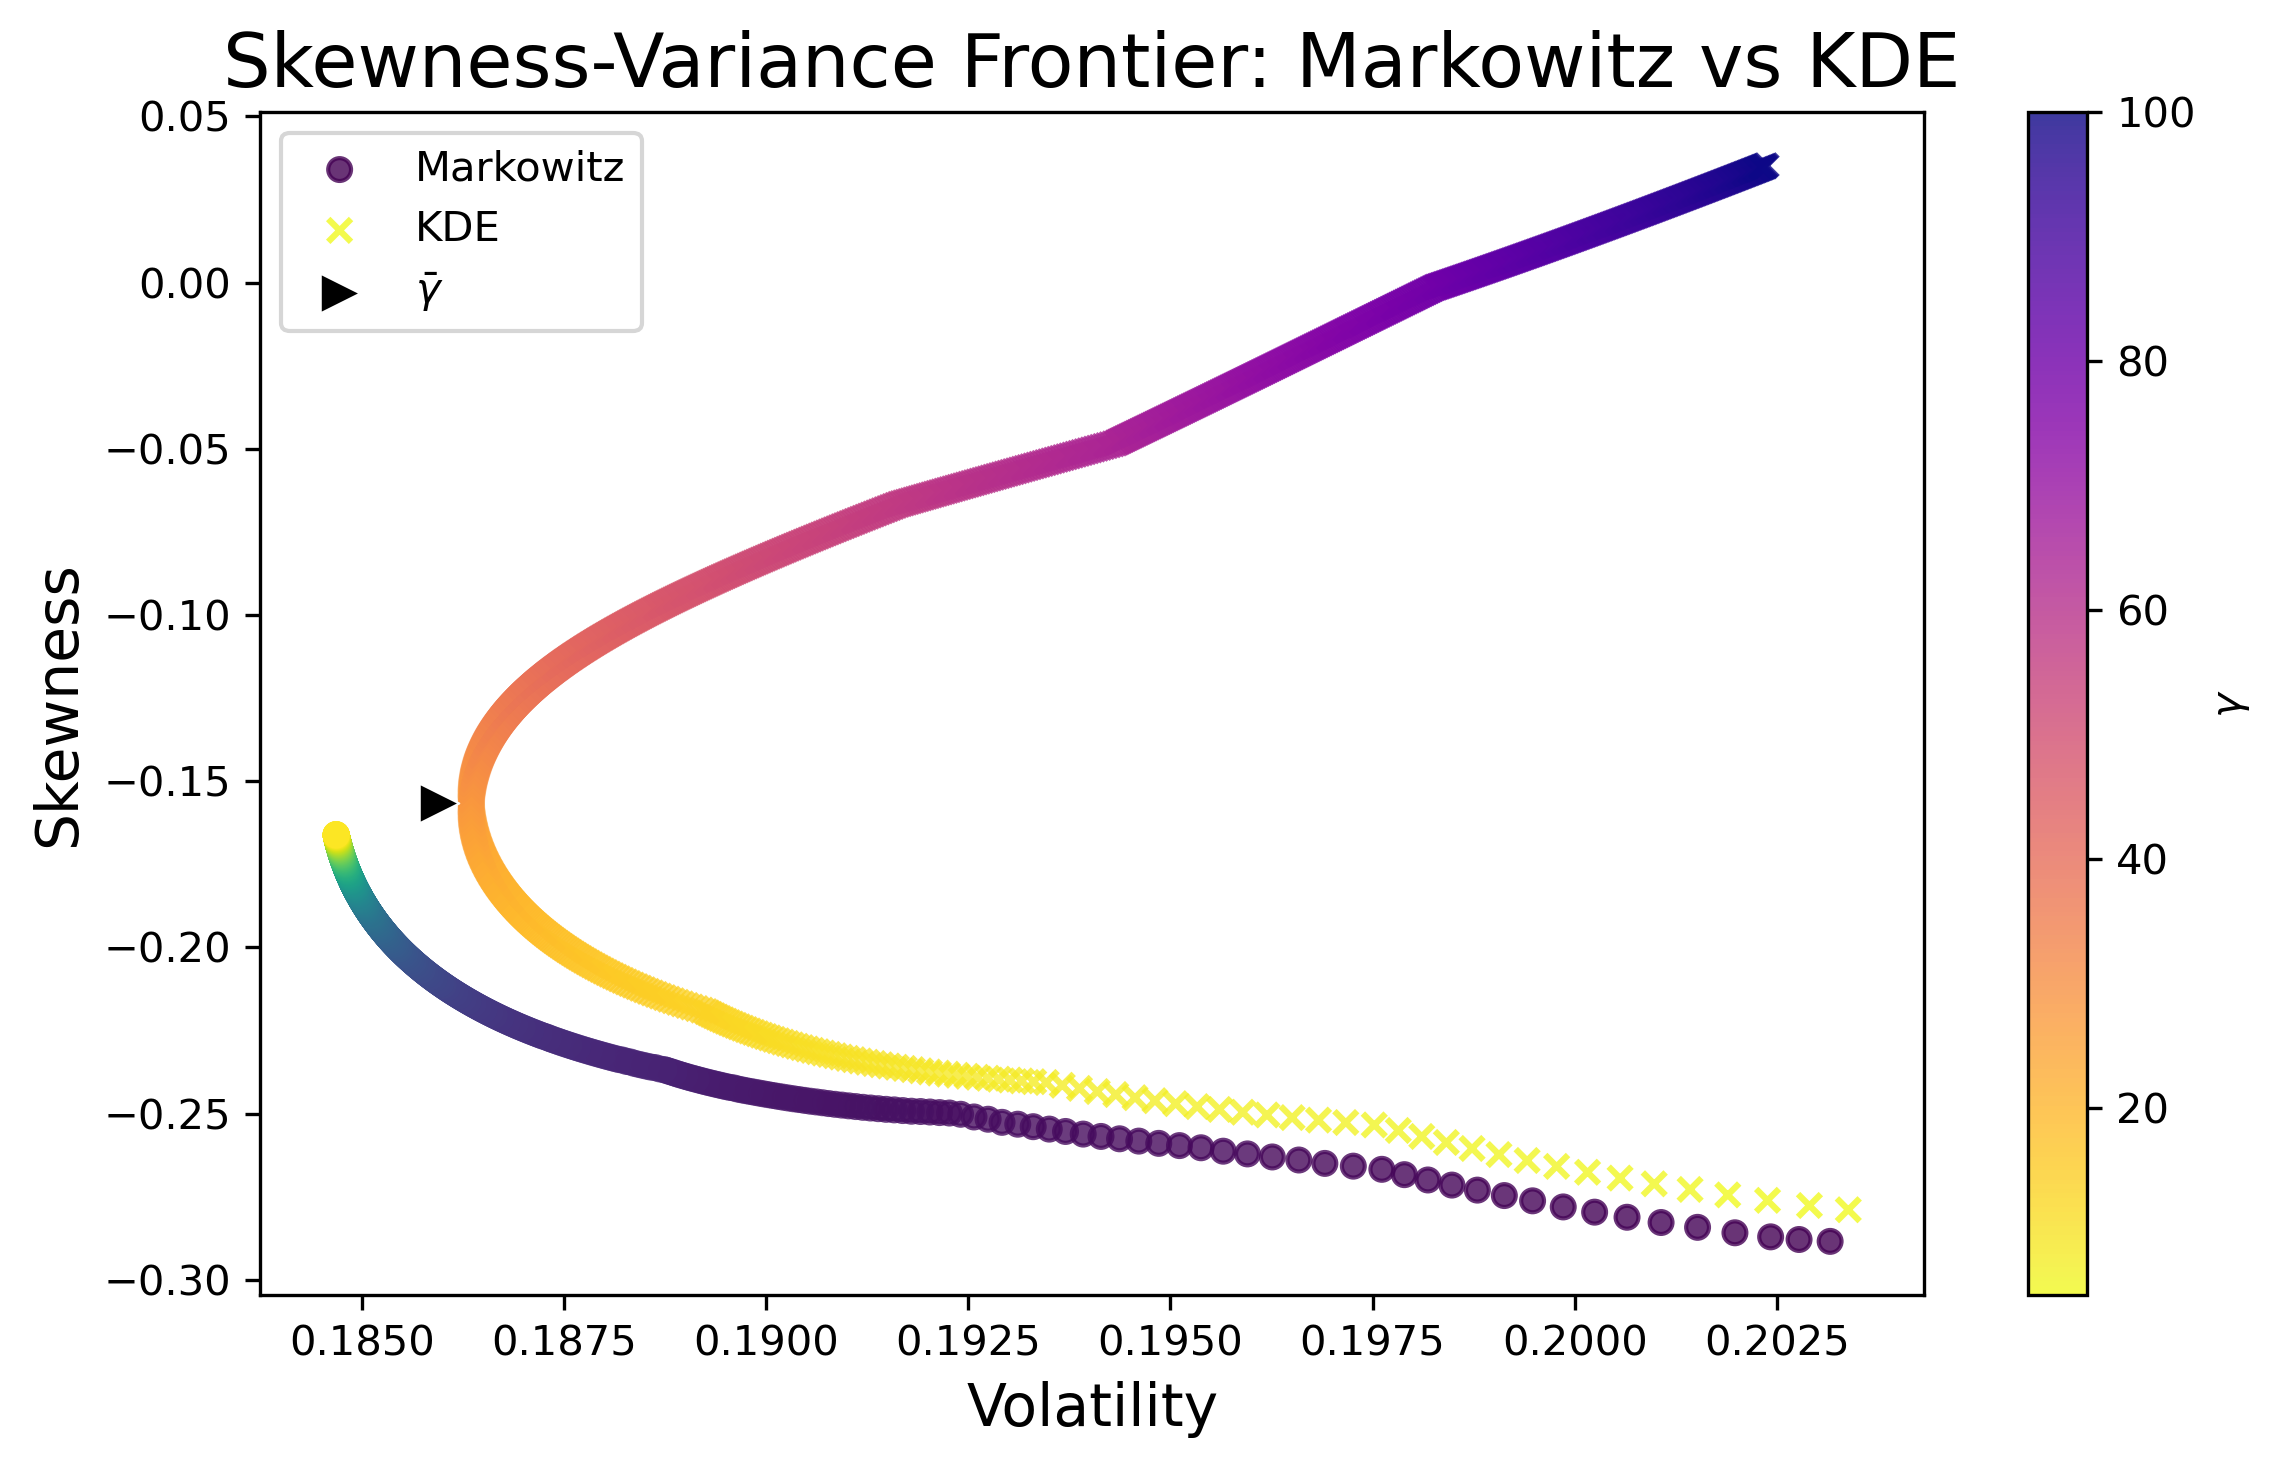
\includegraphics[width=0.65\textwidth]{images/30_2.png}
    \end{minipage}
    \caption[Skewness-variance frontier: Markowitz vs KDE]{Skewness-variance efficient frontiers. Here, the x-axis shows portfolio variance and the y-axis shows ex-post portfolio return skewness, with markers colored by $\gamma$ (yellow to purple). All other details are the same as in Figure \ref{fig:frontier1}.}

    \label{fig:frontier2}
    \end{center}
    \end{figure}

\newpage
As risk aversion increases, KDE initially approaches the Markowitz minimum variance portfolio but never reaches it. This occurs because the KDE optimization implicitly balances variance reduction against skewness improvement. At the point corresponding to $\bar{\gamma}$, the KDE minimum variance portfolio represents an equilibrium between these competing objectives, not a true global minimum in portfolio variance. Beyond this threshold, the priority for skewness improvement begins to dominate, causing the frontier to reverse direction along the volatility axis. This is the second reason why the volatility of the KDE minimum variance portfolio exceeds that of its Markowitz counterpart: it has already been implicitly incorporating skewness throughout the optimization process, compromising some variance reduction to achieve more favorable higher-moment characteristics.

Let us formally define a threshold of risk aversion $\bar{\gamma} > 0$ on the KDE mean-variance frontier corresponding to the KDE minimum-variance portfolio. Along the KDE frontier, all optimal portfolios with risk aversion $\gamma > \bar{\gamma}$ provide an inferior risk-return tradeoff compared to any portfolio with $\gamma \leq \bar{\gamma}$. Simultaneously, every portfolio in this dominated region exhibits higher skewness than any portfolio with $\gamma \leq \bar{\gamma}$. 

Thus, portfolios in the region where $\gamma > \bar{\gamma}$ simultaneously exhibit: (a) inferior mean-variance characteristics, and (b) superior variance-skewness attributes. This establishes a fundamental tension between competing criteria of portfolio efficiency and leads us to the following propositions:

\begin{proposition}\label{prop:skew-var}
Increasing the skewness of a portfolio beyond that of the minimum variance portfolio necessarily requires accepting a higher level of portfolio variance.
\end{proposition}

\begin{proposition}\label{prop:skew-sharpe}
Increasing the skewness of a portfolio beyond that of the minimum variance portfolio necessarily requires accepting a lower risk-return (mean-variance) profile than would have otherwise been attainable.
\end{proposition}

\begin{proposition}\label{prop:counterpoint}
Contrary to the prediction of the Markowitz framework, rational investors with the highest levels of risk aversion ($\gamma > \bar{\gamma}$) should not prefer the minimum variance portfolio, but should instead select portfolios with higher variance that offer improved skewness characteristics, thereby reducing exposure to extreme negative outcomes.
\end{proposition}

\subsection{Effect of H on KDE portfolios}
\label{sec:honkde}
Inspecting the effect of the variation in bandwidth on the KDE frontiers reveals a surprising result: the bandwidth parameter may be unimportant in the context of portfolio optimization. Figure \ref{fig:frontier3} demonstrates this by comparing efficient frontiers across multiple bandwidth scales.

\vspace{5mm}
\begin{figure}[H]
    \begin{center}
    \begin{minipage}{1\textwidth}
      \centering
      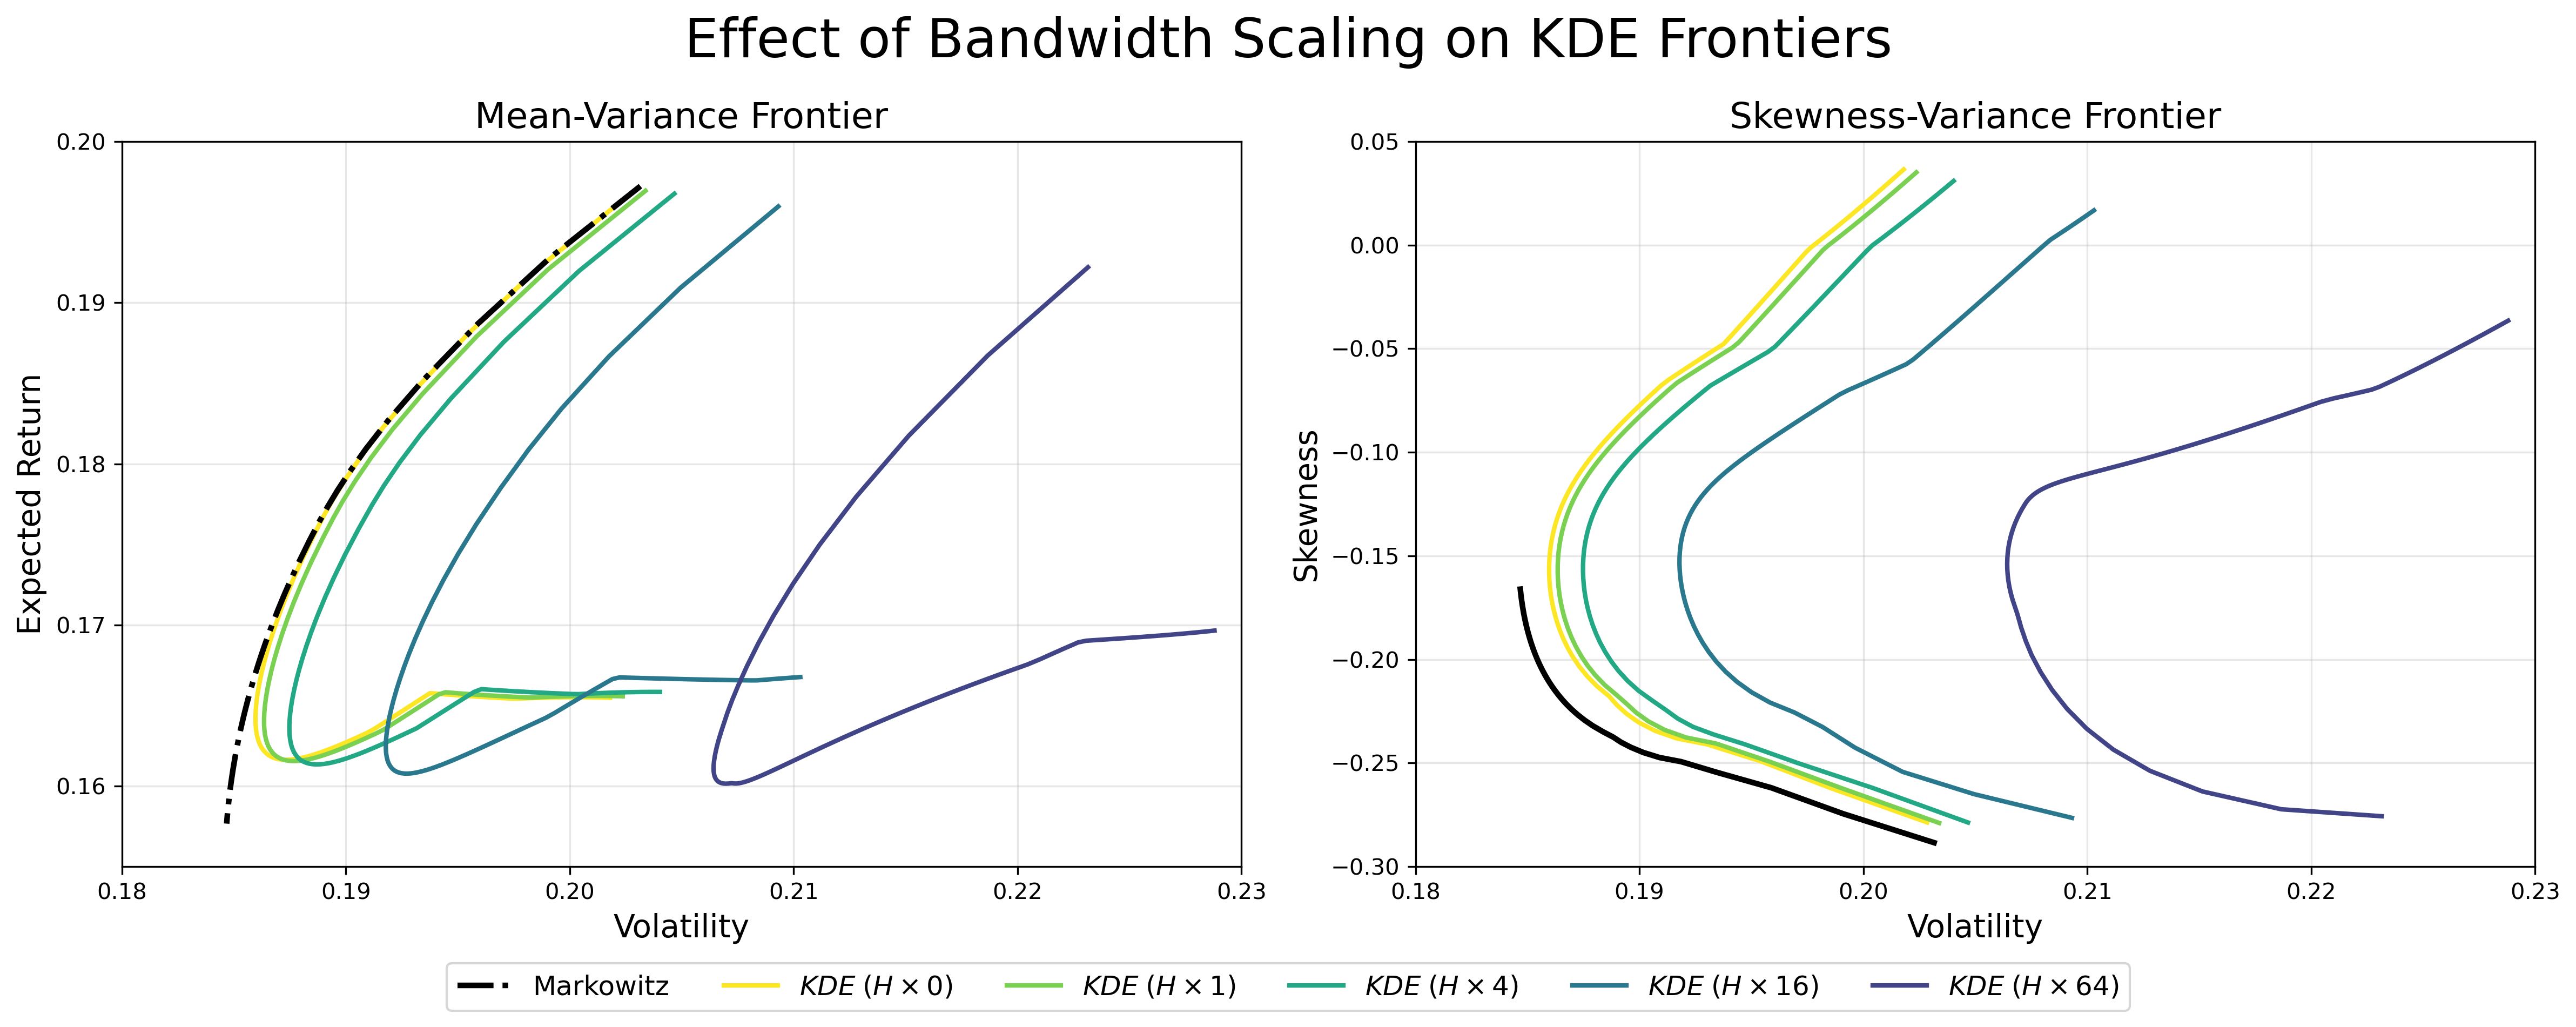
\includegraphics[width=\textwidth]{images/30_3.png}
    \end{minipage}
    \caption[Mean/Skewness-variance frontiers: KDE - Changing $H$]{Effect of bandwidth scaling on KDE-based efficient frontiers for $\gamma\in[5,100]$. \emph{Left:} Mean-variance frontier showing classical Markowitz (black dash-dotted) and KDE frontiers at $H\times\{0,1,4,16,64\}$ (colored solid lines, from light to dark). \emph{Right:} Corresponding skewness-variance frontier comparing the same curves, with skewness on the vertical axis. Increasing the bandwidth scale smooths the density estimate and shifts both frontiers, flattening the mean-variance curve and raising skewness at the cost of higher variance.}
    \label{fig:frontier3}
    \end{center}
    \end{figure}

In KDE, the quadratic term $\tfrac12\gamma^{2}\mathbf w^{\mathsf{T}}H\mathbf w$ sits inside the utility objective, while the ex-ante portfolio variance is $\sigma^{2}(\mathbf w)=\mathbf w^{\mathsf{T}}(H+\Sigma)\mathbf w$. Enlarging $h$ inflates both expressions, so for any fixed $\gamma$, the optimal variance $\sigma^{2}$ moves to the right. The shift is purely mechanical because a wider kernel leads to a stronger penalty on taking additional risk.

When $h=0$, the quadratic penalty disappears from the objective, and the low-$\gamma$ end of the KDE frontier coincides exactly with the Markowitz mean-variance frontier. More importantly, the entire $h=0$ frontier dominates all $h>0$ frontiers in variance-skew space, i.e., extra smoothing reduces improvements in skewness without delivering lower variance. This suggests that the bias-variance tradeoff logic of KDE does not translate into better portfolios.

Furthermore, $h$ and $\gamma$ are effectively substitutes. A larger $h$ lowers the critical risk aversion $\bar\gamma$ at which the KDE attains its lowest volatility. This is because a larger $H$ makes reductions in variance more costly, so a smaller increment in $\gamma$ switches the optimizer from variance-first to skewness-first. 

For the data set we study, the unsmoothed case $(H=0)$ already enables sensitivity to skewness through the adaptive weights $p_i$, and additional bandwidth appears only to reduce the effectiveness of this mechanism. Therefore, practitioners can consider skipping the bandwidth calibration step altogether. If bandwidth is removed from the objective function, KDE loses its interpretation as a tool for smoothing a discrete analytical function and becomes instead a convex backtest.

\subsection{Effect of K on GMM}
\label{sec:kongmm}
Figure \ref{fig:frontier4} presents efficient frontiers for GMM optimization across an increasing number of mixture components $K\in\{1,2,4,8,16\}$. The results reveal a more erratic pattern compared to the systematic behavior observed with KDE.

\vspace{5mm}
\begin{figure}[H]
    \begin{center}
    \begin{minipage}{1\textwidth}
      \centering
      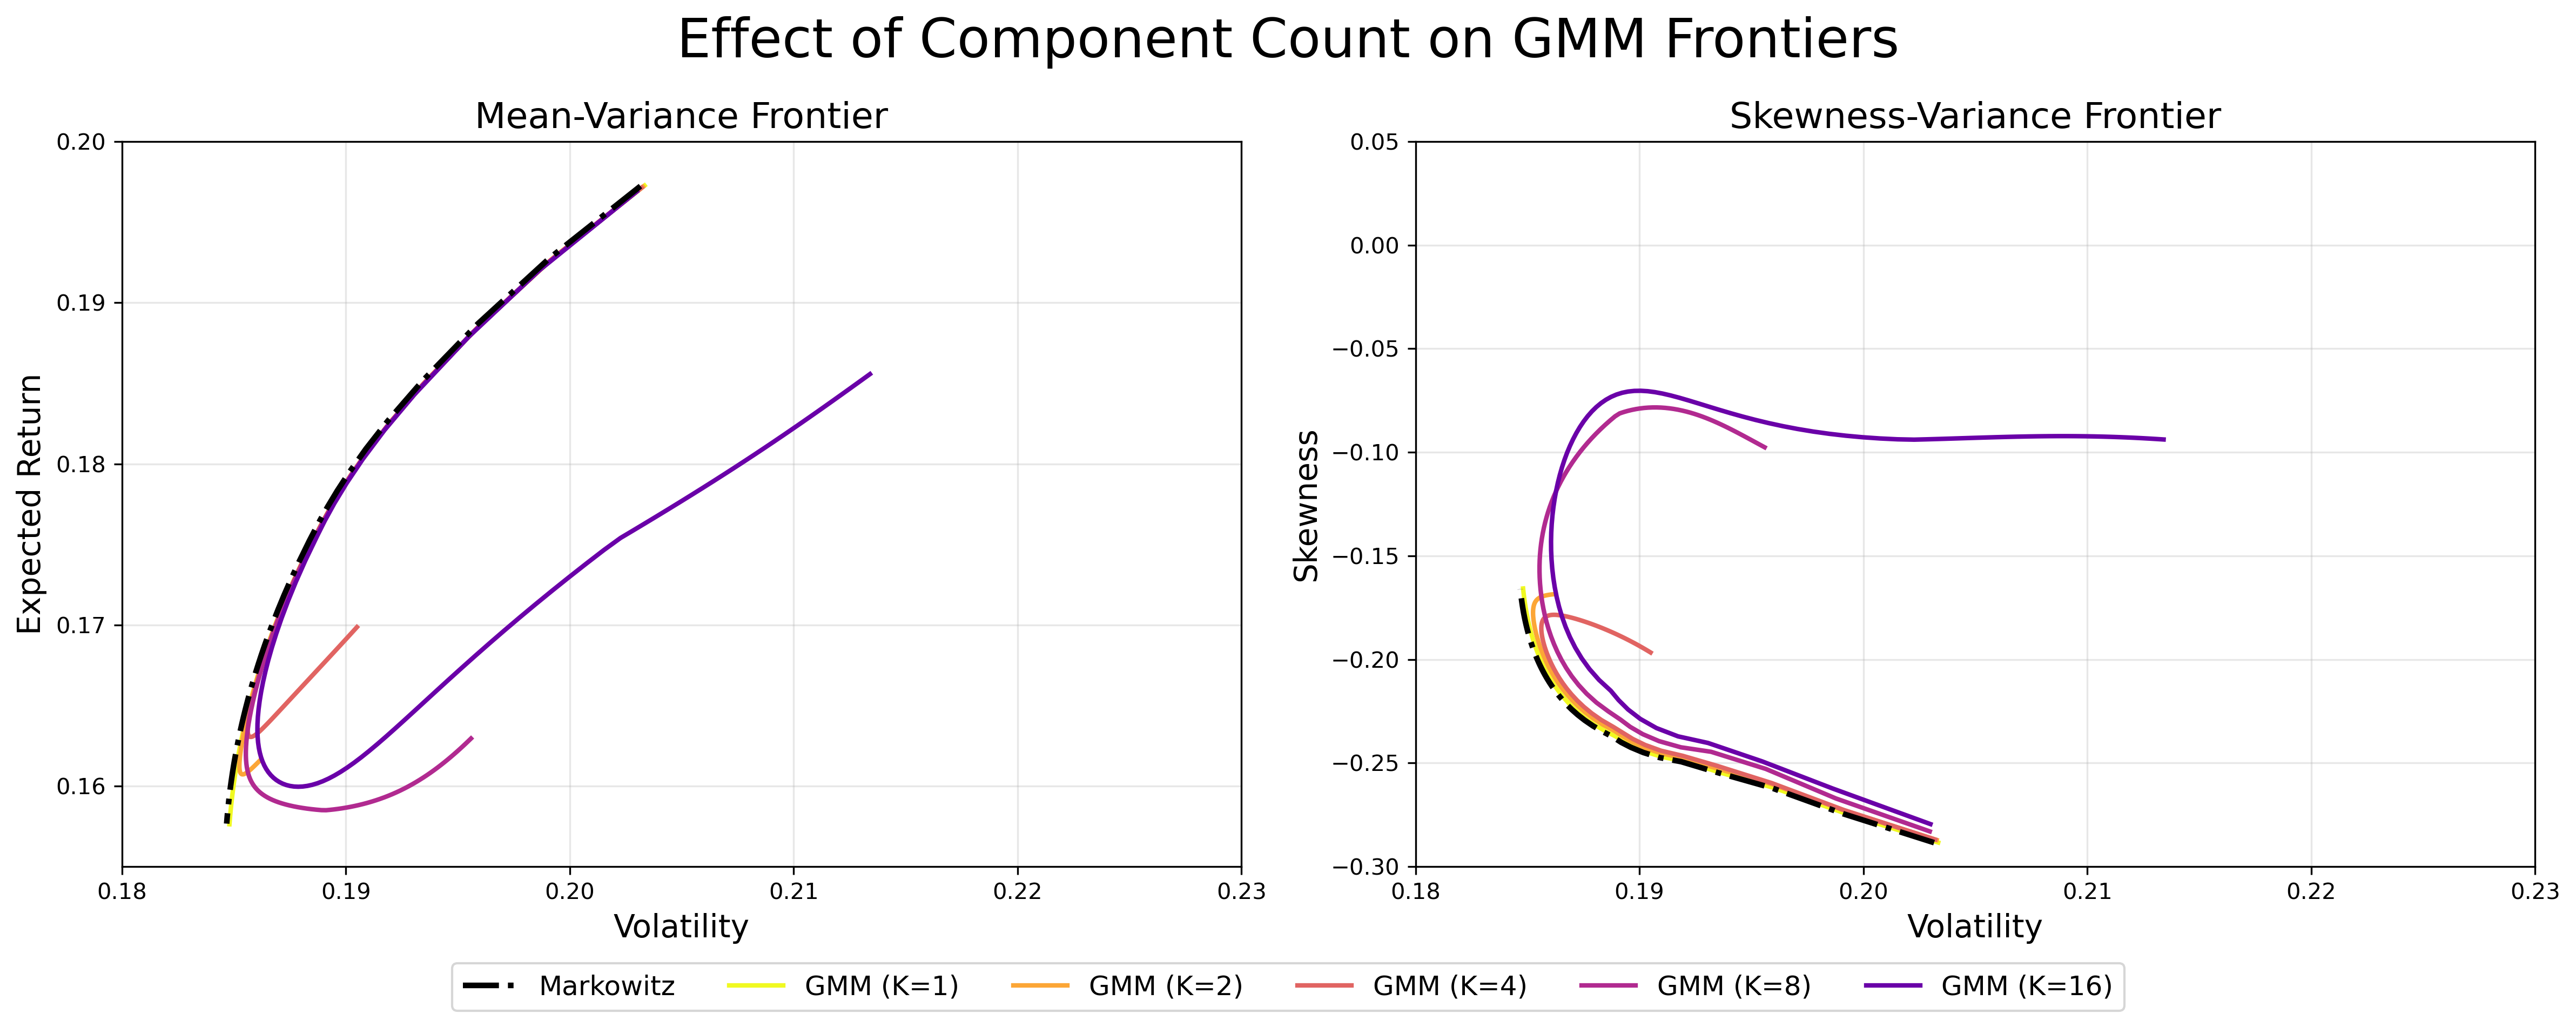
\includegraphics[width=\textwidth]{images/30_4.png}
    \end{minipage}
    \caption[Mean/Skewness-variance frontiers: GMM - Changing $K$]{Same format as Figure \ref{fig:frontier3}, but showing GMM efficient frontiers for varying numbers of mixture components $K\in\{1,2,4,8,16\}$. Figure bounds are unchanged.}
    \label{fig:frontier4}
    \end{center}
    \end{figure}

As expected, the $K=1$ frontier exactly reproduces the Markowitz frontier, representing a single multivariate normal distribution. Higher values of $K$ generate frontiers that qualitatively resemble KDE, with dominated regions in mean-variance space, where both expected return and volatility increase with risk aversion. However, the relationship between component count and frontier performance lacks the consistency observed with bandwidth scaling in KDE.

The $K=16$ frontier achieves the best mean-variance profile, with a steeper and more extended dominated region than other specifications. This steepness suggests that GMM potentially offers a superior return-volatility tradeoff. However, this advantage comes at a cost: all GMM frontiers substantially underperform KDE in the skew-variance space. Unlike KDE, where skewness continuously improves with increasing risk aversion, GMM frontiers tend to fold upon themselves, resulting in higher volatility and no skewness improvement beyond certain risk aversion levels.

These results suggest higher component counts are preferable. At the same time, increasing $K$ introduces significant computational complexity, especially for larger portfolios. With $K=16$ components potentially assigning a separate multivariate normal to each asset in our sample, GMM begins to resemble KDE conceptually, but with the crucial limitation of forcing individual assets into elliptical distributions.

\newpage
Thus, GMM occupies an awkward middle ground. It captures some non-normality benefits but lacks the ability to mitigate skewness like KDE. The inconsistent performance across different $K$ values, coupled with the computational requirements, makes GMM less attractive than either standard Markowitz (for simplicity) or KDE (for skewness improvement).

\subsection{Summary}
The frontier analysis demonstrates three key findings. First, KDE optimization establishes a clear tradeoff between mean-variance efficiency and skewness improvement, with portfolios beyond the critical risk aversion $\bar{\gamma}$ sacrificing mean-variance efficiency to achieve better skewness characteristics. Second, bandwidth selection in KDE appears largely inconsequential, with the unsmoothed case ($H=0$) delivering superior performance through its adaptive weighting mechanism alone. Third, GMM optimization shows inconsistent performance across different component counts and fails to match KDE's skewness improvements despite increased computational complexity. The empirical analysis that follows will examine how these theoretical properties translate into out-of-sample performance.
\chapter{Empirical Analysis}
\label{chap:empirical}
\lhead{Chapter 4. \emph{Empirical Analysis}}

\section{Data and Methodology}
This analysis aims to evaluate the performance characteristics of the GMM and KDE portfolios and compare them to those of the standard strategies. To do so, we compare the out-of-sample performance of these strategies when deployed on the S\&P500, FTSE100, STOXX50, and the HSI indices. We also perform tests on the subsets of these indices to see whether the performance characteristics are affected by the number of assets in the portfolio. To this end, we attempt every combination of the following meta-parameters:
\begin{itemize}
\item \textbf{Data frequency:} daily, weekly, monthly
\item \textbf{Portfolio rebalancing frequency:} monthly, annual
\item \textbf{Data window size:} 1, 3 and 6 months; 1, 3, 5 and 10 years.
\item \textbf{Number of assets in portfolio:} 5, 10, 20, 30, or the maximum available in the index. For the S\&P500 we also have 100 and 450.
\end{itemize}

This implies 210 possible combinations for the FTSE100, STOXX50, and the HSI indices. Given the large allowable number of assets, the total number of possible configurations for the S\&P500 is 294. However, not all configurations yield stable or reliable results due to the relationship between sample size and portfolio dimensionality.

To address this issue, we compute a window-density metric for each configuration:
$$\text{window-density} = \frac{\text{\# return observations in the look-back window}}{\text{\# assets in the universe}}$$

Configurations with very sparse data (window-density < 10\%) are discarded because they produce unstable estimates and spuriously disperse out-of-sample performance. This filtering criterion removes configurations such as "6 monthly observations with 450 assets" on the S\&P500 and all one-month windows with weekly or monthly data frequency.

After applying this filter, our final dataset consists of 828 unique configurations across the four indices: FTSE100 (194 configurations), HSI (196 configurations), S\&P500 (242 configurations), and STOXX50 (196 configurations).

For the full index investment, we use the in-time daily time series of the index composition. At every rebalancing period, the strategy observes the composition of the index being replicated and uses the historical returns data for the current constituents. If no data is available for a given constituent, it is removed from the investment set on that iteration. Still, the constituents' inclusion is nonetheless reattempted in the next rebalancing period. 

For the portfolios that use subsets of the entire index, we randomly sample a set of assets in the very first period. The selected assets then constitute our portfolio for the following periods. It will frequently be the case that previously selected assets will churn out of the index; in this circumstance, we randomly select new assets to replace those dropped. 

It is important to note that a single random selection of assets from the index would not suffice to provide statistically robust results, as we risk selecting unusually performing constituents. For this reason, evaluating subsampled portfolios requires us to draw multiple times per configuration. We use Python's built-in $\textit{random}$ module to make the random selection. For every draw, we provide a random seed corresponding to the count of that iteration, i.e., $\text{Random Seed}_i = i-1$. The returns data for that iteration are then stored and named such that the index, configuration, and the random seed used can be deduced from the file name.

In the analysis that follows, when we talk about the performance of a particular configuration, we talk about the averaged performance metrics across all the $i$ random seeds. The only exception is the full index performance since no subsampling is performed.

\subsection{Limitations and Caveats}
\label{sec:introlimitations}
Our empirical analysis has several limitations. Specifically, the analysis focuses solely on long-only, fully invested portfolios applied to four large indices. It does not account for transaction costs or portfolio turnover, primarily due to practical constraints related to data storage. Additionally, minimum-variance strategies for KDE and GMM are not included, given the complexity of deriving closed-form solutions. For KDE portfolios, the bandwidth parameter is restricted to positive values ($H>0$). These caveats are discussed comprehensively in Section \ref{sec:limitations}, along with suggested improvements for future research.


\section{Baseline Results}
\subsection{Benchmarks}
Given the four strategies that we propose, it is appropriate to evaluate them against multiple benchmark portfolios. The standard mean-variance Markowitz portfolio (MAR), parameterized by risk aversion $\gamma$, serves as the natural counterpart to the GMM and KDE portfolios, with all three evaluated at the same level of risk aversion ($\gamma$=10). Similarly, the Markowitz tangency portfolio (TAN) acts as the benchmark for TAN(GMM) and TAN(KDE), as all three aim to maximize the Sharpe Ratio. We also include the value-weighted (VW) and minimum-variance (MV) portfolios to broaden the comparison.

We begin by comparing the average performance of the five benchmarks - VW, MV, MAR, and TAN - aggregated across all four indices and the full configuration space. Performance is evaluated using the following core metrics: mean return ($\mu$), standard deviation ($\sigma$), Sharpe ratio ($SR$), cumulative return ($CR$), the 95\% Value-at-Risk ($VaR$), maximum drawdown ($DD$), and the duration of the maximum drawdown ($|DD|$). The values for $\mu$, $\sigma$, $SR$, and $VaR$ are annualized. All performance metrics cover the 10-year period from January 2015 to March 2025. Table \ref{tab:single1} and Figure \ref{fig:combined2} summarize the benchmark performance metrics. (Per index tables available in the Appendix \ref{app:avgperf}). $|DD|$ is excluded from the radar chart for visual clarity.
\vspace{5mm}
\begin{table}[H]
  \centering
  \begin{tabular}{l*{7}{S[table-format=1.4]}}
  \toprule
  & {$\mu$} & {$\sigma$} & {SR} & {CR} & {VaR} & {DD} & {\textbar DD\textbar} \\
  \midrule
  VW & 0.0982 & 0.1814 & {\bfseries 0.4370} & {\bfseries 1.3317} & 0.2687 & 0.3534 & {\bfseries 3.0056} \\
  MV & 0.0849 & {\bfseries 0.1669} & 0.3895 & 1.0771 & {\bfseries 0.2423} & {\bfseries 0.3475} & 3.4809 \\
  MAR & {\bfseries 0.1922} & 0.2125 & 0.3645 & 1.2629 & 0.3143 & 0.4174 & 4.0214 \\
  TAN & 0.1885 & 0.1996 & 0.3817 & 1.2292 & 0.2950 & 0.3909 & 3.6075 \\
  \bottomrule
\end{tabular}

  \caption[Benchmark performance]{Annualized performance of benchmark portfolios (Jan 2015-Mar 2025), averaged across all indices. Maximum drawdown and $VaR$ are shown in absolute terms; boldface entries indicate the best performer in each metric.}
  \label{tab:single1}
\end{table}

\begin{figure}[H]
\begin{center}
\begin{minipage}{0.48\textwidth}
  \centering
  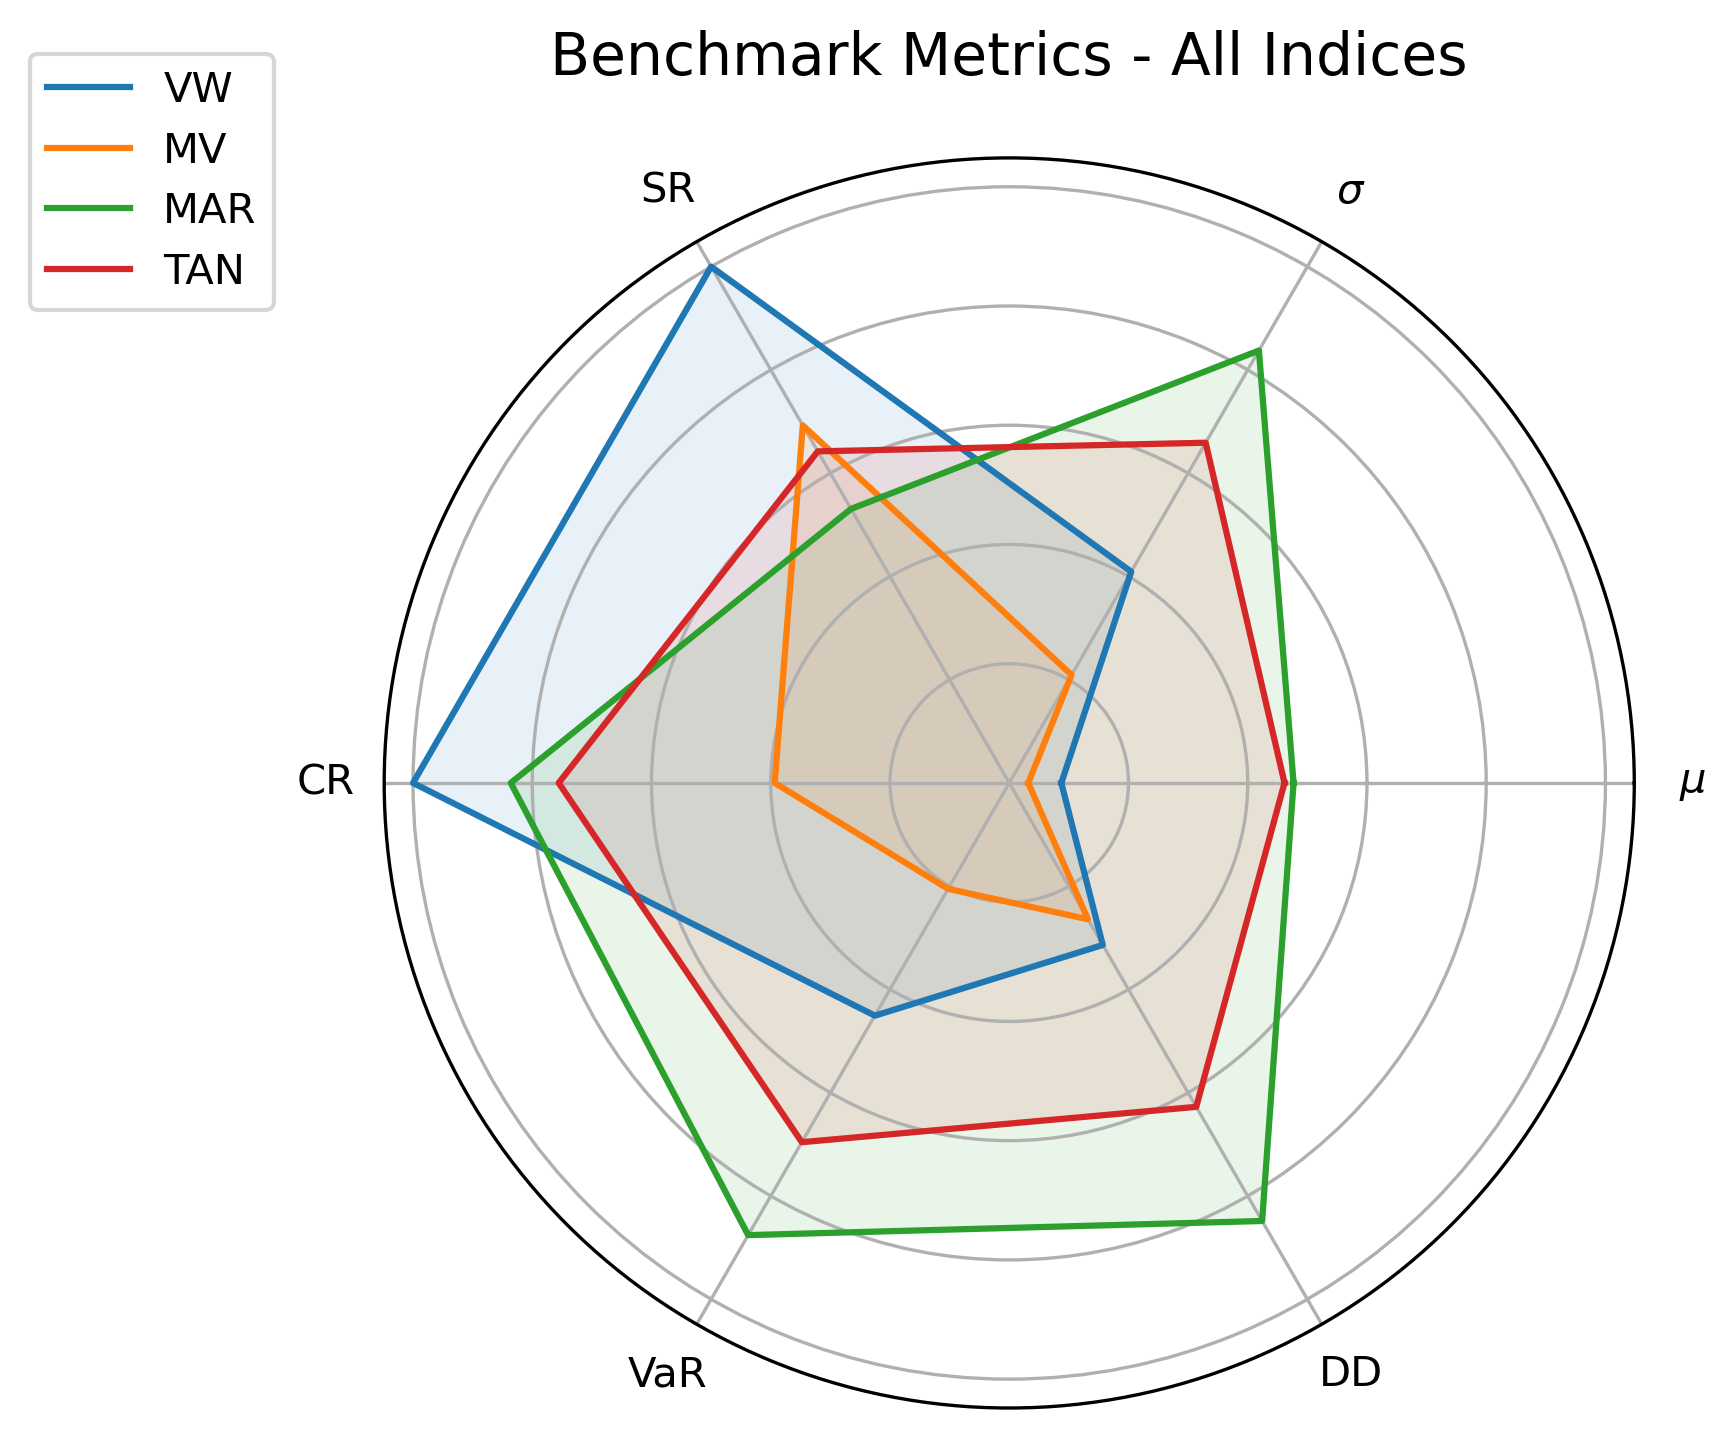
\includegraphics[width=\textwidth]{images/40_1.png}
\end{minipage}
\hfill
\begin{minipage}{0.48\textwidth}
  \centering
  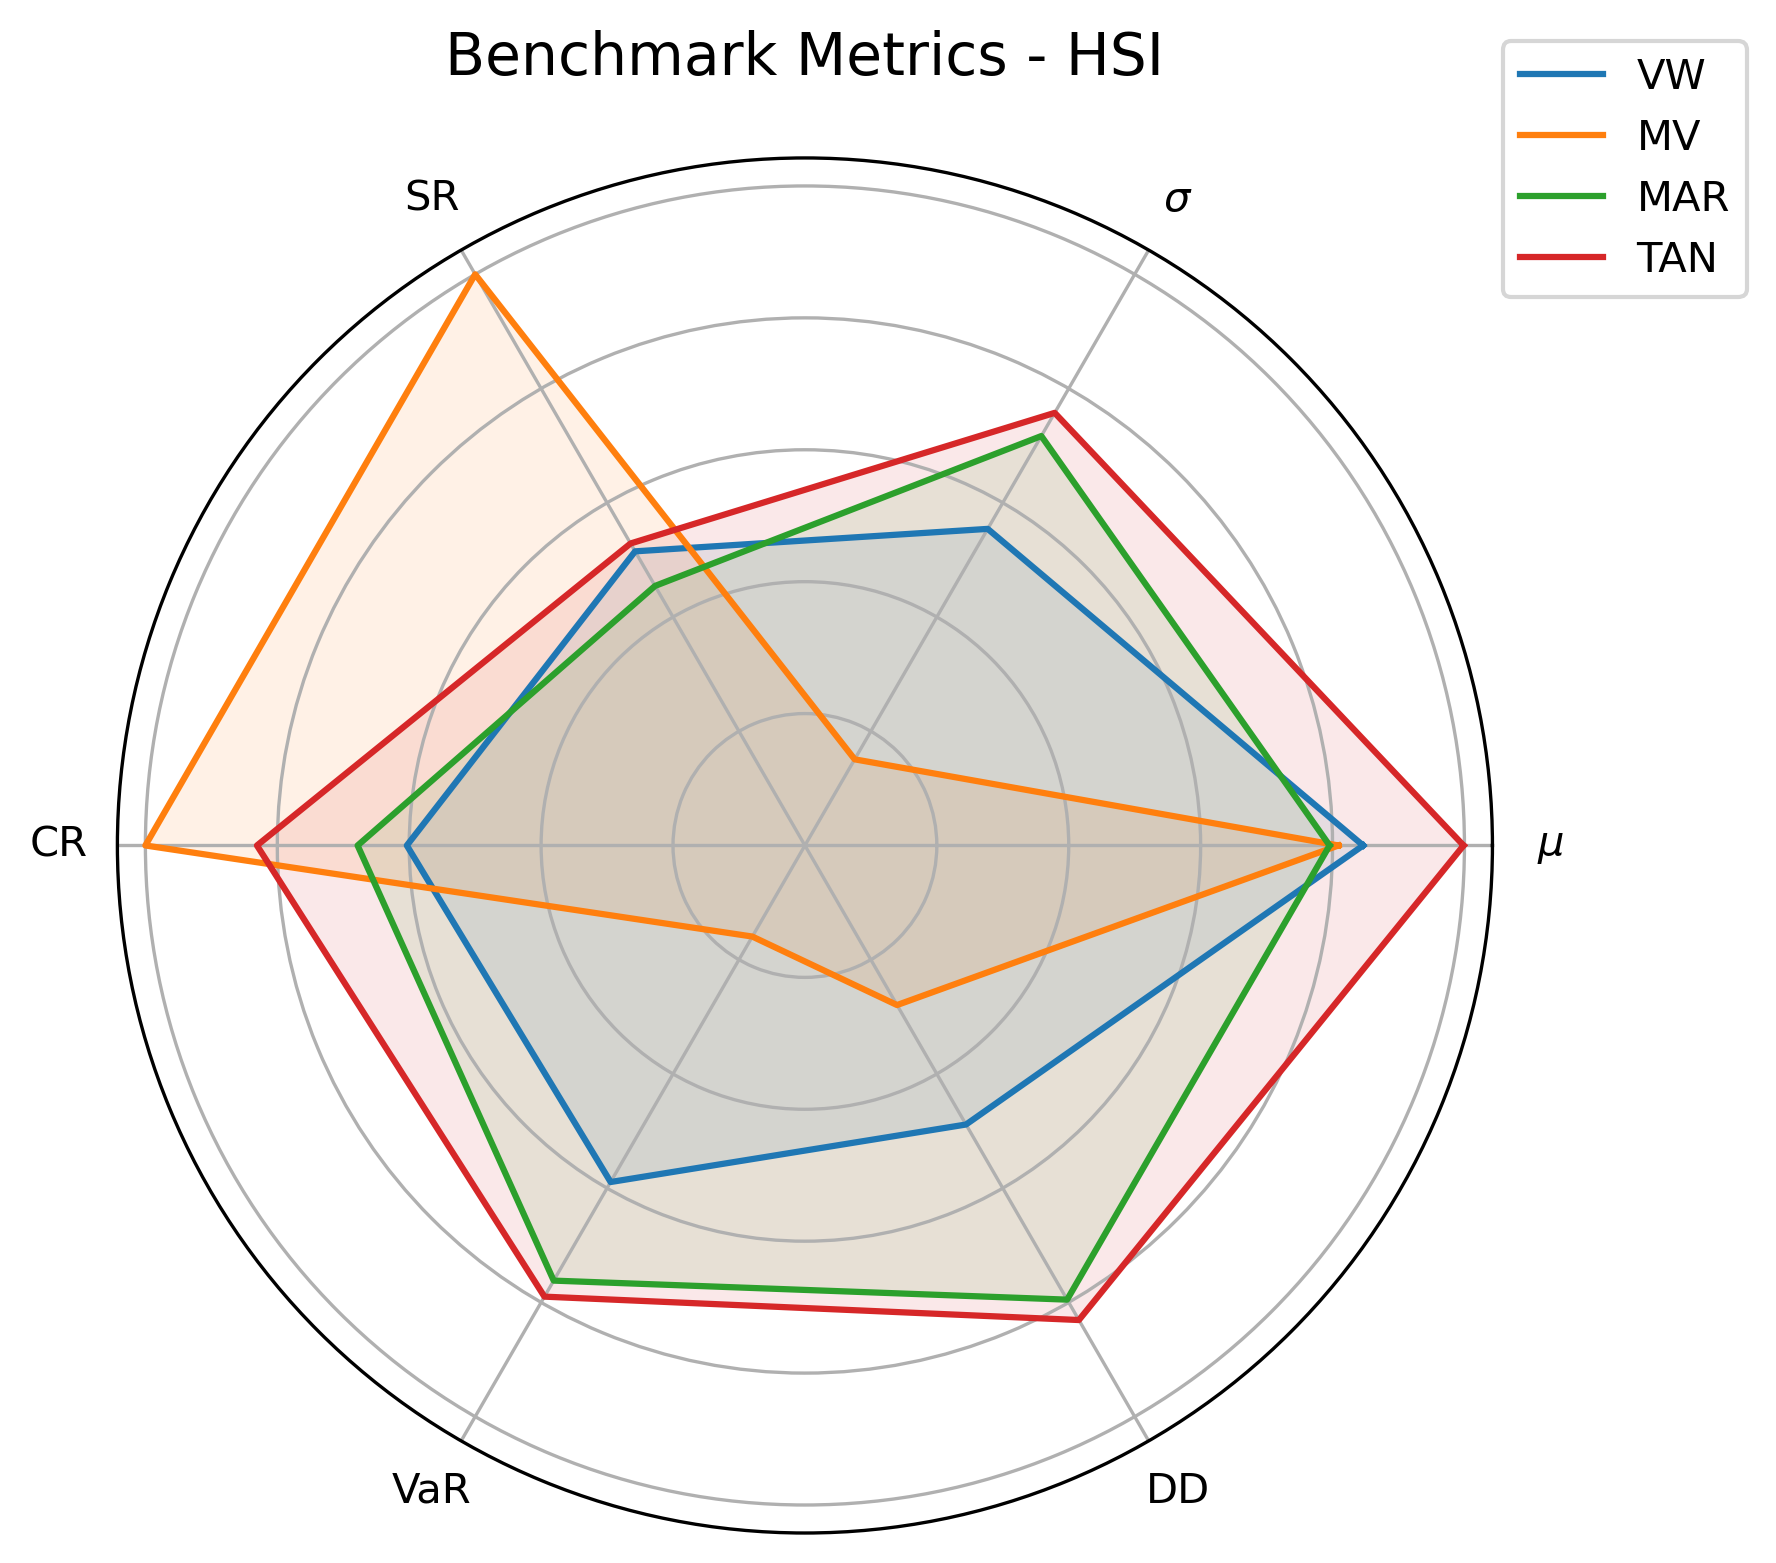
\includegraphics[width=\textwidth]{images/40_2.png}
\end{minipage}
\caption[Benchmark performance - Radar]{Performance comparison of benchmark portfolios (VW (blue); MV (orange); MAR (green) and TAN (red)) across six metrics: annualized return ($\mu$), volatility ($\sigma$), Sharpe ratio (SR), cumulative return (CR), 95\% VaR, and maximum drawdown (DD). All axes are scaled so that a larger radius indicates better performance; "bad" metrics ($\sigma$, VaR, DD) have been inverted.}
\label{fig:combined2}
\end{center}
\end{figure}

From these, we make several observations:
\begin{itemize}
\item The VW portfolios consistently offered the best trade-off between cumulative returns and the Sharpe Ratio. VW portfolios achieved the highest overall $SR$ in all indices except the HSI.
\item The MV portfolios offered the lowest $\sigma$ and $VaR$ across the board. Although MV did not record the lowest $DD$ in every index, a significant comparative improvement in drawdowns relative to other portfolios in the HSI index ensured that MV had the lowest $DD$ on average.
\item The MAR and TAN portfolios delivered the highest returns, but at the cost of high volatility, elevated $VaR$, and long drawdowns. Their risk profiles were so unfavorable that they ended up with lower ex-post Sharpe Ratios than the MV portfolio.
\end{itemize}
  
Due to the distinct behavior of the HSI index, where the usual performance patterns across benchmarks broke down, we include a separate radar plot focusing exclusively on HSI. Unlike the other indices, HSI saw the MV portfolio dominate across all metrics except $\mu$. The VW portfolio, typically one of the better performers, also struggled in HSI. While it still outperformed most return-optimized strategies in terms of $SR$ and $DD$, its advantage in cumulative return diminished. This contrast attests to the importance of evaluating portfolio performance across multiple indices, as each market may emphasize different strengths and weaknesses in a given strategy. Optimal strategy configurations will be discussed in detail in Section \ref{sec:localoptima}

\subsection{Standard GMM and KDE Results}
On average, the KDE portfolio behaved like a slightly riskier version of MV, achieving a modestly higher cumulative return at the cost of increased volatility. More notably, KDE outperformed MAR, its direct mean-variance counterpart, across all risk-focused metrics. It delivered a higher average Sharpe Ratio, lower volatility, and lower $VaR$, making it a meaningful improvement over the traditional approach. That said, KDE still lagged behind the value-weighted portfolio in terms of $CR$ and $SR$, despite offering a slight decrease in $\sigma$ and $VaR$.
\vspace{5mm}
\begin{table}[H]
  \centering
  \begin{tabular}{l*{7}{S[table-format=1.4]}}
  \toprule
  & {$\mu$} & {$\sigma$} & {SR} & {CR} & {VaR} & {DD} & {\textbar DD\textbar} \\
  \midrule
  VW & 0.0982 & 0.1814 & {\bfseries 0.4370} & {\bfseries 1.3317} & 0.2687 & 0.3534 & {\bfseries 3.0056} \\
  MV & 0.0849 & {\bfseries 0.1669} & 0.3895 & 1.0771 & {\bfseries 0.2423} & {\bfseries 0.3475} & 3.4809 \\
  MAR & {\bfseries 0.1922} & 0.2125 & 0.3645 & 1.2629 & 0.3143 & 0.4174 & 4.0214 \\
  KDE & 0.0853 & 0.1726 & 0.3801 & 1.0827 & 0.2529 & 0.3491 & 3.5437 \\
  GMM & 0.1737 & 0.2059 & 0.3107 & 1.0032 & 0.2986 & 0.4125 & 4.3024 \\
  \bottomrule
\end{tabular}

  \caption[Benchmark vs. KDE/GMM performance]{Annualized performance of benchmark, KDE, and GMM portfolios (Jan 2015-Mar 2025), averaged across all indices. Same metrics as in Table \ref{tab:single1}.}
  \label{tab:single2}
\end{table}

\begin{figure}[H]
\begin{center}
\begin{minipage}{1\textwidth}
  \centering
  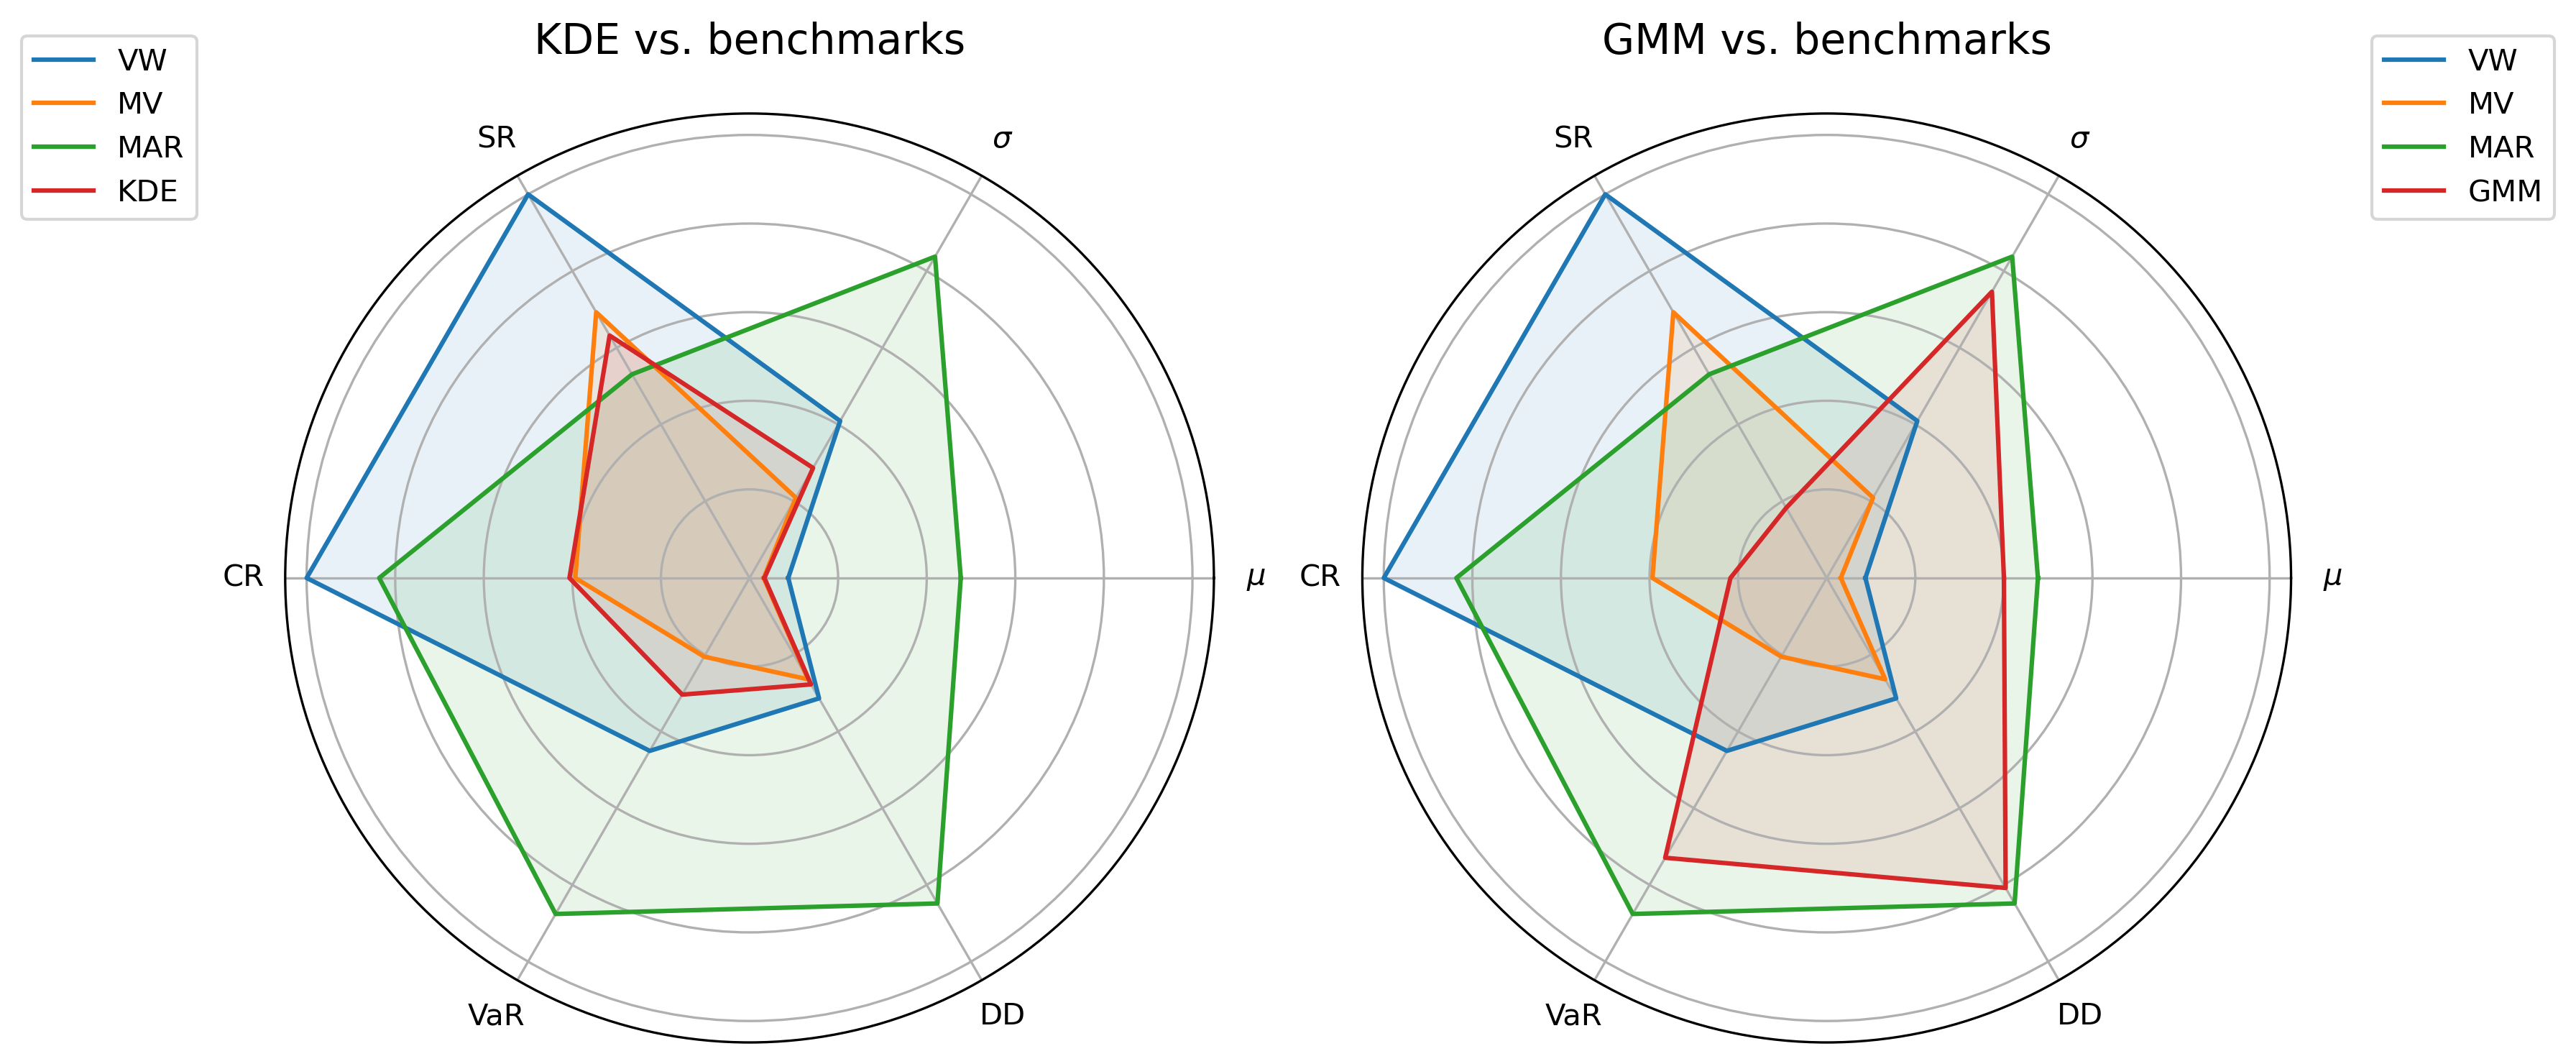
\includegraphics[width=\textwidth]{images/40_3.png}
\end{minipage}
\caption[Benchmark vs. KDE/GMM performance - Radar]{Radar-plot comparison of KDE (red, left) and GMM (red, right) portfolios against benchmark strategies VW (blue), MV (orange), and MAR (green). Same axes as in Figure \ref{fig:combined2}. The left panel shows the KDE portfolio, while the right panel shows the GMM portfolio.}
\label{fig:combined3}
\end{center}
\end{figure}

The GMM portfolio exhibited a return profile similar to that of MAR, but with noticeably worse risk-adjusted performance. While GMM improved slightly on all risk metrics compared to MAR, it still delivered the lowest cumulative return among all strategies, lower than that of the minimum-variance portfolio. As a result, its Sharpe Ratio was significantly lower than all other portfolios. Compared to the value-weighted, MV, and KDE portfolios, GMM's performance was disappointing. While it did achieve higher mean returns, it fell behind in every other metric and delivered an unattractive risk-return profile.

While the VW portfolio appears to dominate in this comparison, it is too early to draw definitive conclusions about the effectiveness of the KDE and GMM methods. The VW portfolio benefits from using the same information across all configurations, whereas KDE and GMM are sensitive to the data available within each setting. Hence, the averaged results presented here include many configurations with minimal data, making reliable estimation challenging for these density-based approaches. From Section \ref{sec:portability} onwards, we explore performance across different configurations and highlight the conditions under which these methods perform comparatively well.


\subsection{Tangency Portfolios}
\begin{table}[H]
  \centering
  \begin{tabular}{l*{7}{S[table-format=1.4]}}
  \toprule
  & {$\mu$} & {$\sigma$} & {SR} & {CR} & {VaR} & {DD} & {\textbar DD\textbar} \\
  \midrule
  VW & 0.0982 & 0.1814 & {\bfseries 0.4370} & {\bfseries 1.3317} & 0.2687 & 0.3534 & {\bfseries 3.0056} \\
  MV & 0.0849 & {\bfseries 0.1669} & 0.3895 & 1.0771 & {\bfseries 0.2423} & {\bfseries 0.3475} & 3.4809 \\
  TAN & 0.1885 & 0.1996 & 0.3817 & 1.2292 & 0.2950 & 0.3909 & 3.6075 \\
  TAN(KDE) & 0.1891 & 0.1939 & 0.3969 & 1.2379 & 0.2867 & 0.3793 & 3.4441 \\
  TAN(GMM) & {\bfseries 0.3184} & 0.2243 & 0.3266 & 1.0915 & 0.3277 & 0.4355 & 4.2121 \\
  \bottomrule
\end{tabular}

  \caption[Benchmark vs. TAN(KDE)/TAN(GMM) performance]{Annualized performance of benchmark, TAN(KDE), and TAN(GMM) portfolios (Jan 2015-Mar 2025), averaged across all indices. Same metrics as in Table \ref{tab:single1}.}
  \label{tab:single3}
\end{table}

\vspace{5mm}
\begin{figure}[H]
\begin{center}
\begin{minipage}{1\textwidth}
  \centering
  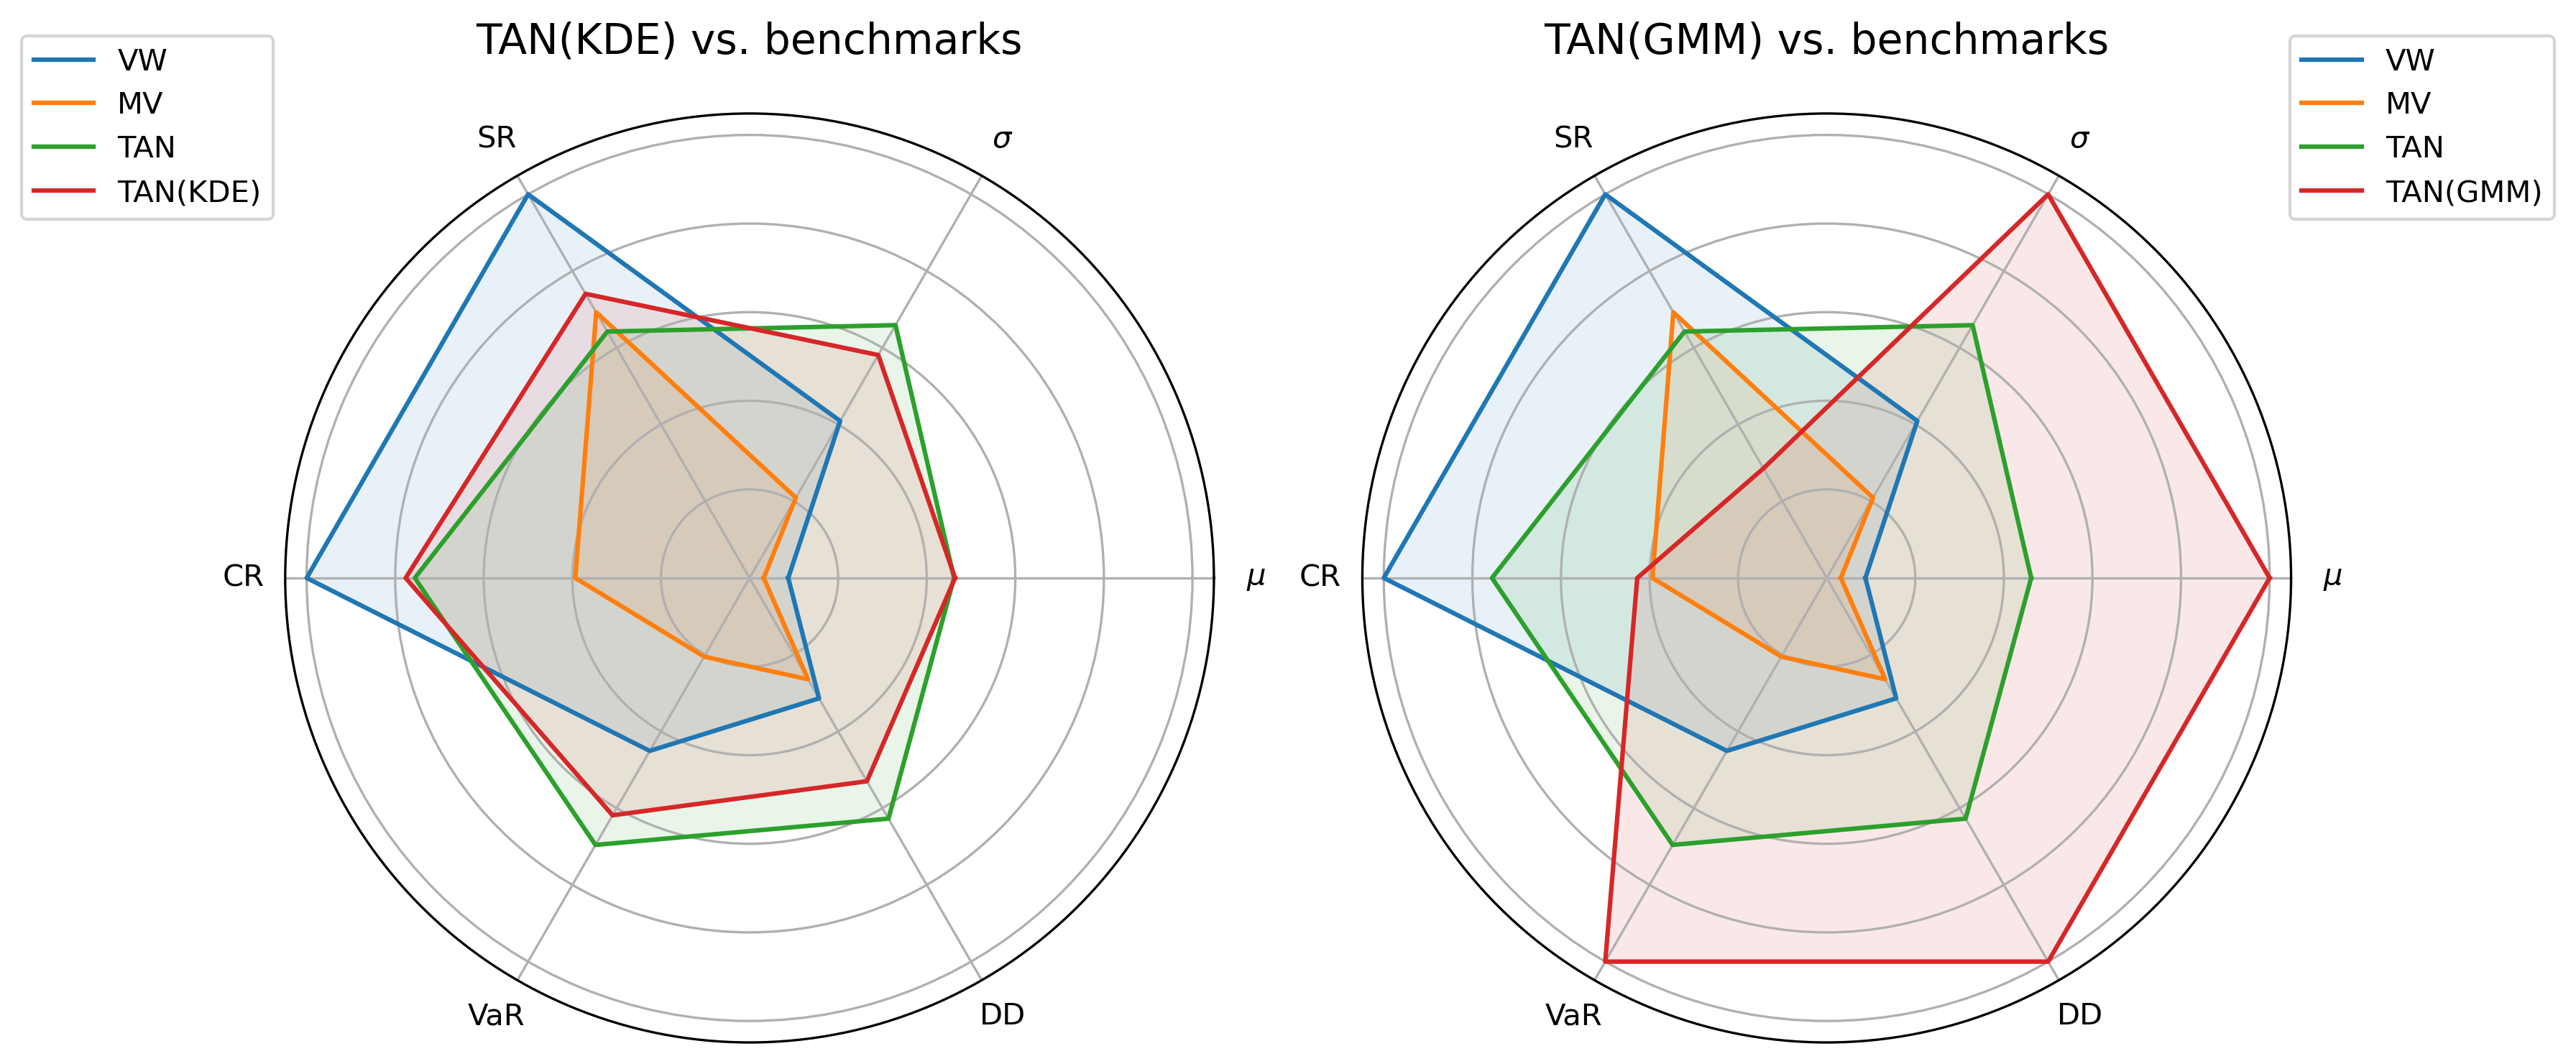
\includegraphics[width=\textwidth]{images/40_4.png}
\end{minipage}
\caption[Benchmark vs. TAN(KDE)/TAN(GMM) performance - Radar]{Radar-plot comparison of TAN(KDE) (red, left) and TAN(GMM) (red, right) portfolios against benchmark strategies VW (blue), MV (orange), and MAR (green). Same axes as in Figure \ref{fig:combined2}. The left panel shows the TAN(KDE) portfolio, while the right panel shows the TAN(GMM) portfolio.}
\label{fig:combined4}
\end{center}
\end{figure}

The TAN(KDE) portfolio delivered strong overall results, achieving the second-highest average Sharpe Ratio across all portfolios. Compared to its direct counterpart, TAN, TAN(KDE) showed a slightly higher cumulative return and Sharpe Ratio, lower volatility, lower Value-at-Risk, and smaller drawdowns. Notably, TAN(KDE) even outperformed the MV portfolio in terms of maximum drawdown within the S\&P500 index, which is surprising given how consistently MV tends to lead on downside risk measures. This performance is especially noteworthy because it emerges despite averaging across all configurations, including many highly data-sparse and inherently challenging for KDE-based estimation. This suggests that TAN(KDE) can deliver a favorable risk-return profile even under varying conditions.

The TAN(GMM) portfolio produced the most extreme results among all strategies. It achieved the highest average mean return, but also the highest volatility, $VaR$, and maximum drawdown. Its risk-adjusted performance was poor despite the strong headline return, with a Sharpe Ratio that fell below that of both TAN and TAN(KDE). Compared to TAN(KDE), it performed worse across every risk metric. In the end, TAN(GMM) managed to maximize not only returns, but also risk.


\section{Strategy Portability}
\label{sec:portability}

Next, we evaluate each portfolio strategy under its most favorable conditions. We define the "best" configuration as the parameter set (data frequency, lookback window, rebalancing interval, and investment universe size) that achieves the highest penalized Sharpe Ratio, averaged across all indices.

The penalized Sharpe Ratio ($SR_p$) balances high average returns against consistency in performance across multiple asset-selection seeds. For portfolio $k$, it is calculated as:
$$SR_{p,k} = \mathbb{E}[SR_k] - \lambda \cdot \sqrt{Var[SR_k]}$$
Or explicitly:
$$SR_{p,k} = \frac{1}{n} \sum_{i=1}^{n} SR_{k,i} - \lambda \cdot \sqrt{ \frac{1}{n} \sum_{i=1}^{n} \left( SR_{k,i} - \frac{1}{n} \sum_{i=1}^{n} SR_{k,i} \right)^2 }$$
Here, $SR_{k,i}$ represents the Sharpe Ratio obtained with seed $i$, and the parameter $\lambda$ controls the penalty imposed for variability across seeds. We use $\lambda=1$, making the penalized Sharpe Ratio the mean Sharpe Ratio minus its standard deviation.

In this Section, we select a single optimal configuration per strategy based on the highest average penalized Sharpe Ratio across all four indices. Identifying a globally effective parameter set and testing it locally allows us to determine how well the strategies generalize. The table below summarizes these optimal configurations ranked by their penalized Sharpe Ratios. Section \ref{sec:localoptima} will discuss index-specific optimal configurations.

\begin{table}[H]
  \centering
  \begin{tabular}{l*{5}{S[table-format=1.4]}}
  \toprule
  & {Reb.} & {Wnd.(mo)} & {Data} & {SR} & {SR$_p$} \\
  \midrule
  VW & {annual} & {5years} & {monthly} & 0.4835 & {\bfseries 0.3788} \\
  MV & {monthly} & {3months} & {daily} & {\bfseries 0.5005} & 0.3773 \\
  KDE & {monthly} & {6months} & {daily} & 0.4714 & 0.3587 \\
  TAN(KDE) & {monthly} & {5years} & {monthly} & 0.4812 & 0.3467 \\
  MAR & {annual} & {1years} & {daily} & 0.4599 & 0.3251 \\
  TAN & {monthly} & {5years} & {monthly} & 0.4624 & 0.3094 \\
  TAN(GMM) & {annual} & {5years} & {monthly} & 0.4071 & 0.2330 \\
  GMM & {monthly} & {1years} & {weekly} & 0.3627 & 0.1947 \\
  \bottomrule
\end{tabular}

  \caption[Best configurations - Global]{Optimal parameter settings per strategy, ranked by average penalized Sharpe ratio across all four indices and portfolio sizes. Columns report rebalancing frequency (Reb.), lookback window in months (Wnd.), data frequency (Data), annualized Sharpe ratio (SR), and penalized Sharpe ratio ($SR_p$). Boldface highlights the best value in each column.}
  \label{tab:single4}
\end{table}

Table \ref{tab:single4} presents the MV portfolio achieving the highest raw Sharpe ratio, while the VW strategy claims the top penalized Sharpe ratio, which demonstrates their superior consistency across different markets. The KDE-based portfolios follow closely, with both vanilla KDE and TAN(KDE) delivering strong risk-adjusted performance. The tangency portfolio using KDE ranks third in Sharpe ratio while posting an average penalized Sharpe ratio. In contrast, the GMM portfolios show weaker performance overall, with both GMM and TAN(GMM) achieving the lowest penalized and raw Sharpe ratios, reflecting high dispersion across configurations.

Having identified the best configuration for each strategy based on global performance, we now evaluate how well these configurations carry over across individual indices.

\begin{center}
  \textbf{FTSE100}
\end{center}
\begin{table}[H]
  \centering
  \begin{tabular}{l*{7}{S[table-format=1.4]}}
  \toprule
  & {$\mu$} & {$\sigma$} & {CR} & {SR} & {VaR} & {DD} & {\textbar DD\textbar} \\
  \midrule
  VW & 0.0736 & 0.1199 & 0.9246 & 0.4455 & 0.1675 & 0.2439 & 1.5833 \\
  MV & 0.0675 & {\bfseries 0.1101} & 0.8185 & 0.4371 & {\bfseries 0.1673} & {\bfseries 0.1914} & {\bfseries 1.2077} \\
  MAR & 0.0768 & 0.2199 & 0.6530 & 0.2602 & 0.3350 & 0.5552 & 6.1615 \\
  TAN & 0.0379 & 0.1404 & 0.3231 & 0.1197 & 0.1921 & 0.3003 & 3.5833 \\
  KDE & 0.1070 & 0.1265 & 1.5705 & {\bfseries 0.6865} & 0.1829 & 0.2826 & 1.2385 \\
  GMM & {\bfseries 0.1171} & 0.1804 & {\bfseries 1.6224} & 0.5432 & 0.2380 & 0.3034 & 2.9423 \\
  TAN(KDE) & 0.0578 & 0.1335 & 0.6241 & 0.2761 & 0.2020 & 0.2767 & 3.4167 \\
  TAN(GMM) & 0.0624 & 0.1648 & 0.6189 & 0.2339 & 0.2734 & 0.3568 & 3.5833 \\
  \bottomrule
\end{tabular}

  \caption[Global best configuration - All strategies - FTSE100]{Annualized performance of all portfolios (Jan 2015-Mar 2025), FTSE100 only. Averaged across all portfolio sizes. Same metrics as in Table \ref{tab:single1}.}
  \label{tab:single5}
\end{table}

In the FTSE100, the MV portfolio significantly outperformed all other strategies in terms of risk management, though its $VaR$ uplift over VW, the second safest portfolio, was marginal. Despite its strong risk metrics, MV did not reach the highest Sharpe Ratio, as its returns remained modest.

\vspace{5mm}
\begin{figure}[H]
  \begin{center}
  \begin{minipage}{1\textwidth}
    \centering
    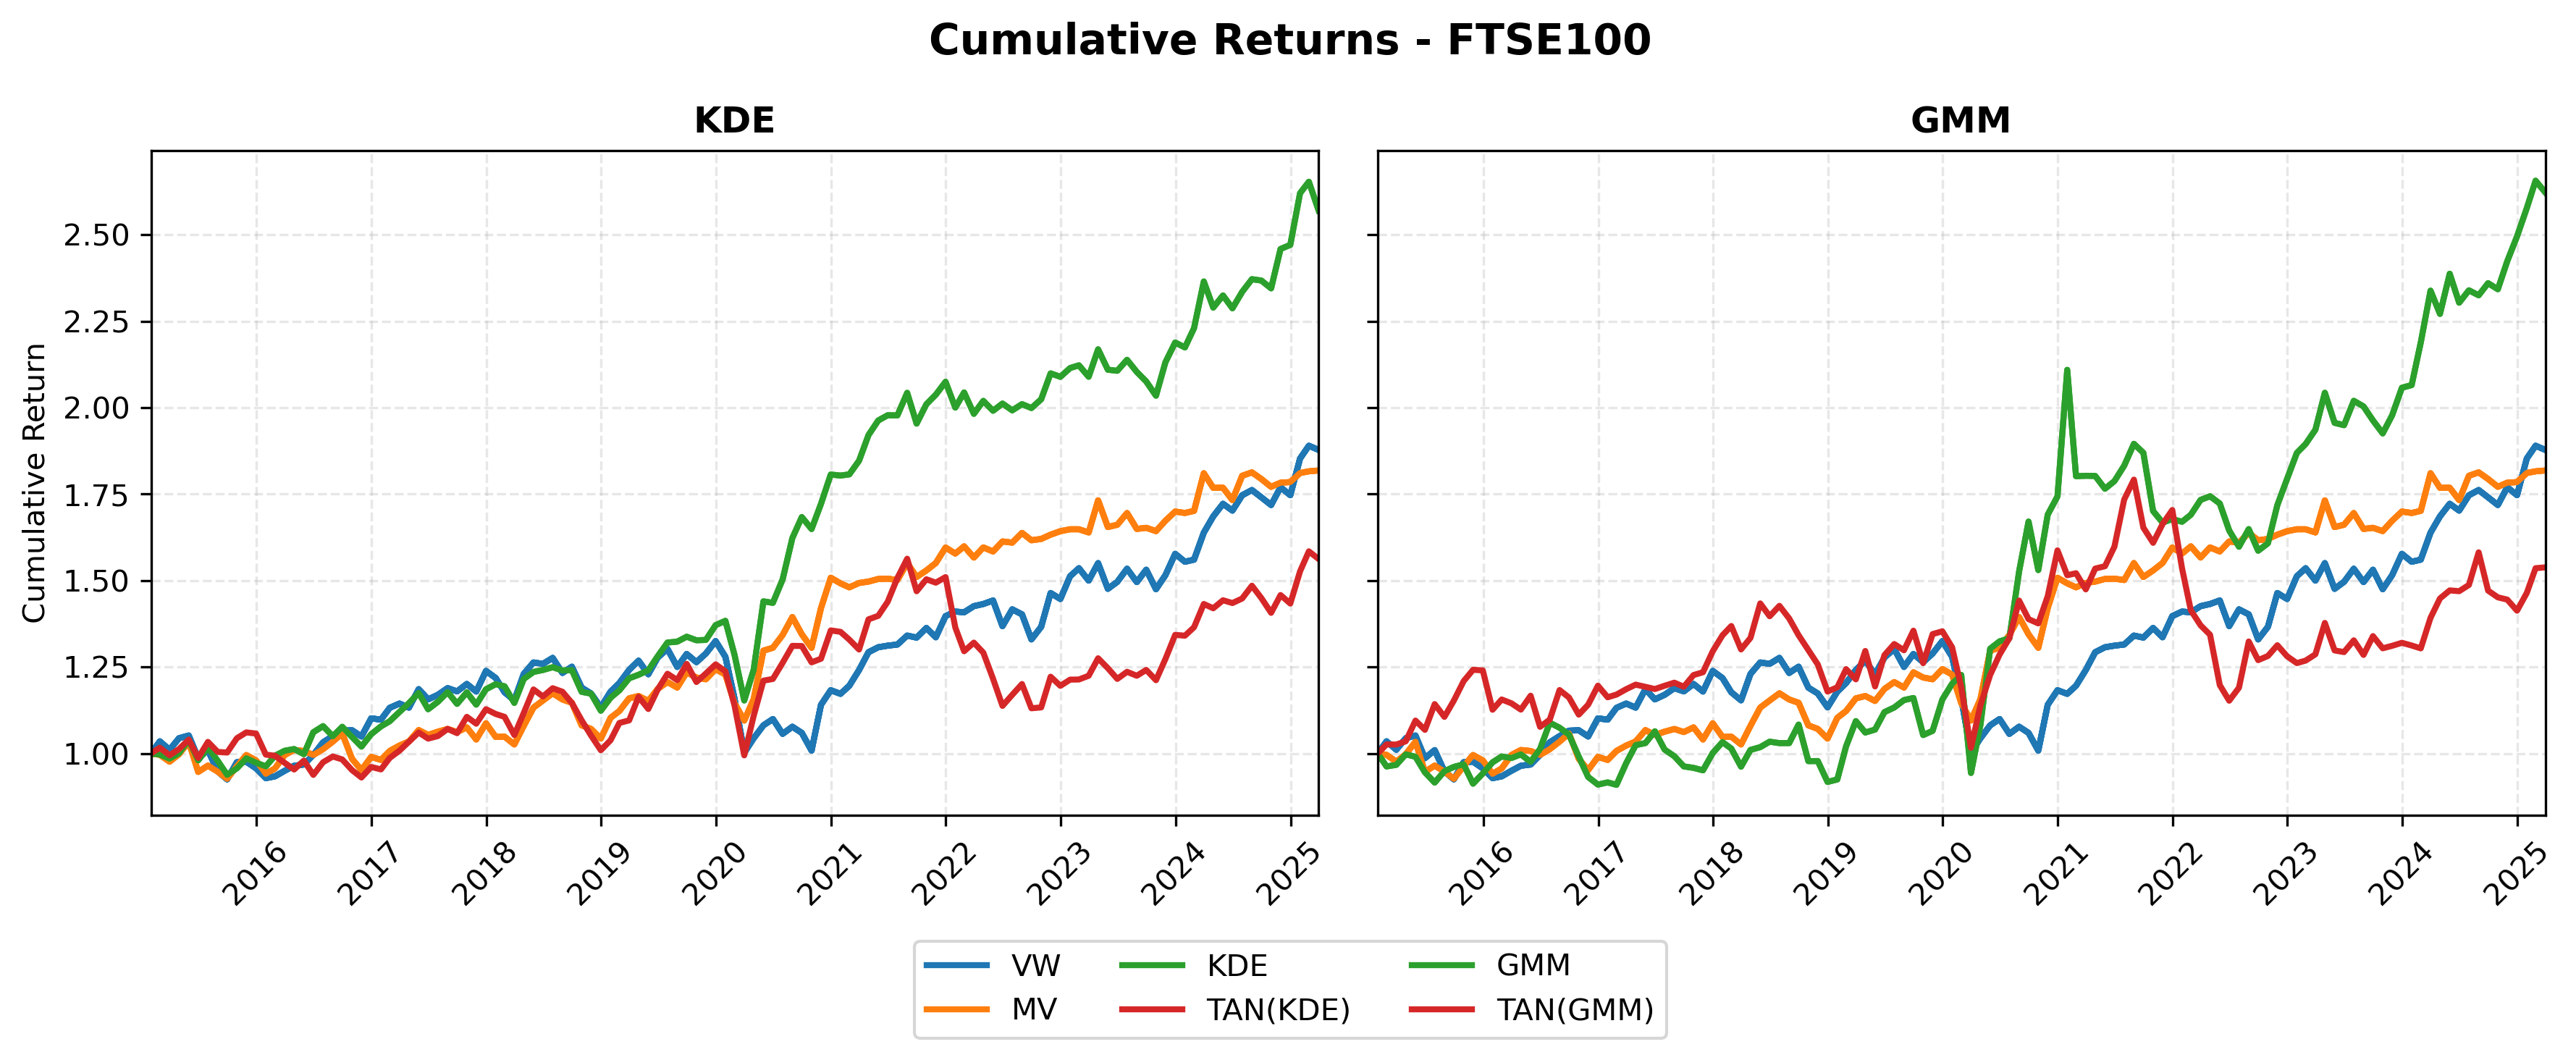
\includegraphics[width=\textwidth]{images/40_6.png}
  \end{minipage}
  \caption[Global best configuration - FTSE100 - Cumulative returns]{Cumulative returns (Jan 2015-Mar 2025) of the best global configuration per strategy on the FTSE100 index. Left panel: default KDE (green) and its tangency variant TAN(KDE) (red) versus benchmarks VW (blue) and MV (orange). Right panel: default GMM (green) and its tangency variant TAN(GMM) (red) versus the same benchmarks. All series are indexed to 1.0 at the start date.}
  \label{fig:combined6}
  \end{center}
  \end{figure}

The KDE portfolio achieved a higher cumulative return than VW and MV, allowing it to outperform them and take the lead in terms of the Sharpe Ratio. However, this came at the cost of worse risk metrics. In contrast, the TAN(KDE) portfolio offered subpar risk metrics and cumulative return. Nevertheless, it had the highest $SR$ among the tangency portfolios, which all performed surprisingly unwell in the FTSE100.

GMM delivers the highest average returns but comes with elevated volatility and $VaR$ that exceed most other strategies. The TAN(GMM) portfolio follows the pattern of tangency underperformance, with substantially lower returns and higher risk metrics than GMM.

% \newpage
\begin{center}
  \textbf{HSI}
\end{center}
In the HSI index, the MV portfolio achieved top-of-the-line performance across the board, leading in all metrics besides mean return and drawdown duration. Surprisingly, the VW portfolio performed poorly, showing the lowest Sharpe Ratio and one of the lowest cumulative returns. This comparative underperformance of VW is unique to the HSI index.

\begin{table}[H]
  \centering
  \begin{tabular}{l*{7}{S[table-format=1.4]}}
  \toprule
  & {$\mu$} & {$\sigma$} & {CR} & {SR} & {VaR} & {DD} & {\textbar DD\textbar} \\
  \midrule
  VW & 0.0593 & 0.2141 & 0.4375 & 0.1391 & 0.3292 & 0.5080 & 4.0833 \\
  MV & 0.0952 & {\bfseries 0.1340} & {\bfseries 1.2643} & {\bfseries 0.5613} & {\bfseries 0.2014} & {\bfseries 0.3036} & 4.8769 \\
  MAR & 0.1006 & 0.2391 & 0.9545 & 0.3366 & 0.3693 & 0.4551 & 6.2231 \\
  TAN & 0.0776 & 0.2191 & 0.6878 & 0.2324 & 0.3531 & 0.5864 & {\bfseries 3.7500} \\
  KDE & 0.0736 & 0.1376 & 0.8471 & 0.3923 & 0.2164 & 0.3791 & 4.7654 \\
  GMM & 0.0432 & 0.1698 & 0.3296 & 0.1380 & 0.2646 & 0.4636 & 6.9615 \\
  TAN(KDE) & 0.0613 & 0.2226 & 0.4317 & 0.1539 & 0.3851 & 0.5999 & {\bfseries 3.7500} \\
  TAN(GMM) & {\bfseries 0.1056} & 0.3890 & 0.4200 & 0.2031 & 0.4020 & 0.7050 & {\bfseries 3.7500} \\
  \bottomrule
\end{tabular}

  \caption[Global best configuration - All strategies - HSI]{Annualized performance of all portfolios (Jan 2015-Mar 2025), HSI only. Averaged across all portfolio sizes. Same metrics as in Table \ref{tab:single1}.}
  \label{tab:single6}
\end{table}

The KDE portfolio improved significantly over VW in both the Sharpe Ratio and cumulative return, while maintaining better downside risk metrics. However, the TAN(KDE) portfolio underperformed, with a lower cumulative return and unattractive risk metrics. This underperformance was shared between all tangency portfolios on the HSI.

\vspace{5mm}
\begin{figure}[H]
  \begin{center}
  \begin{minipage}{1\textwidth}
    \centering
    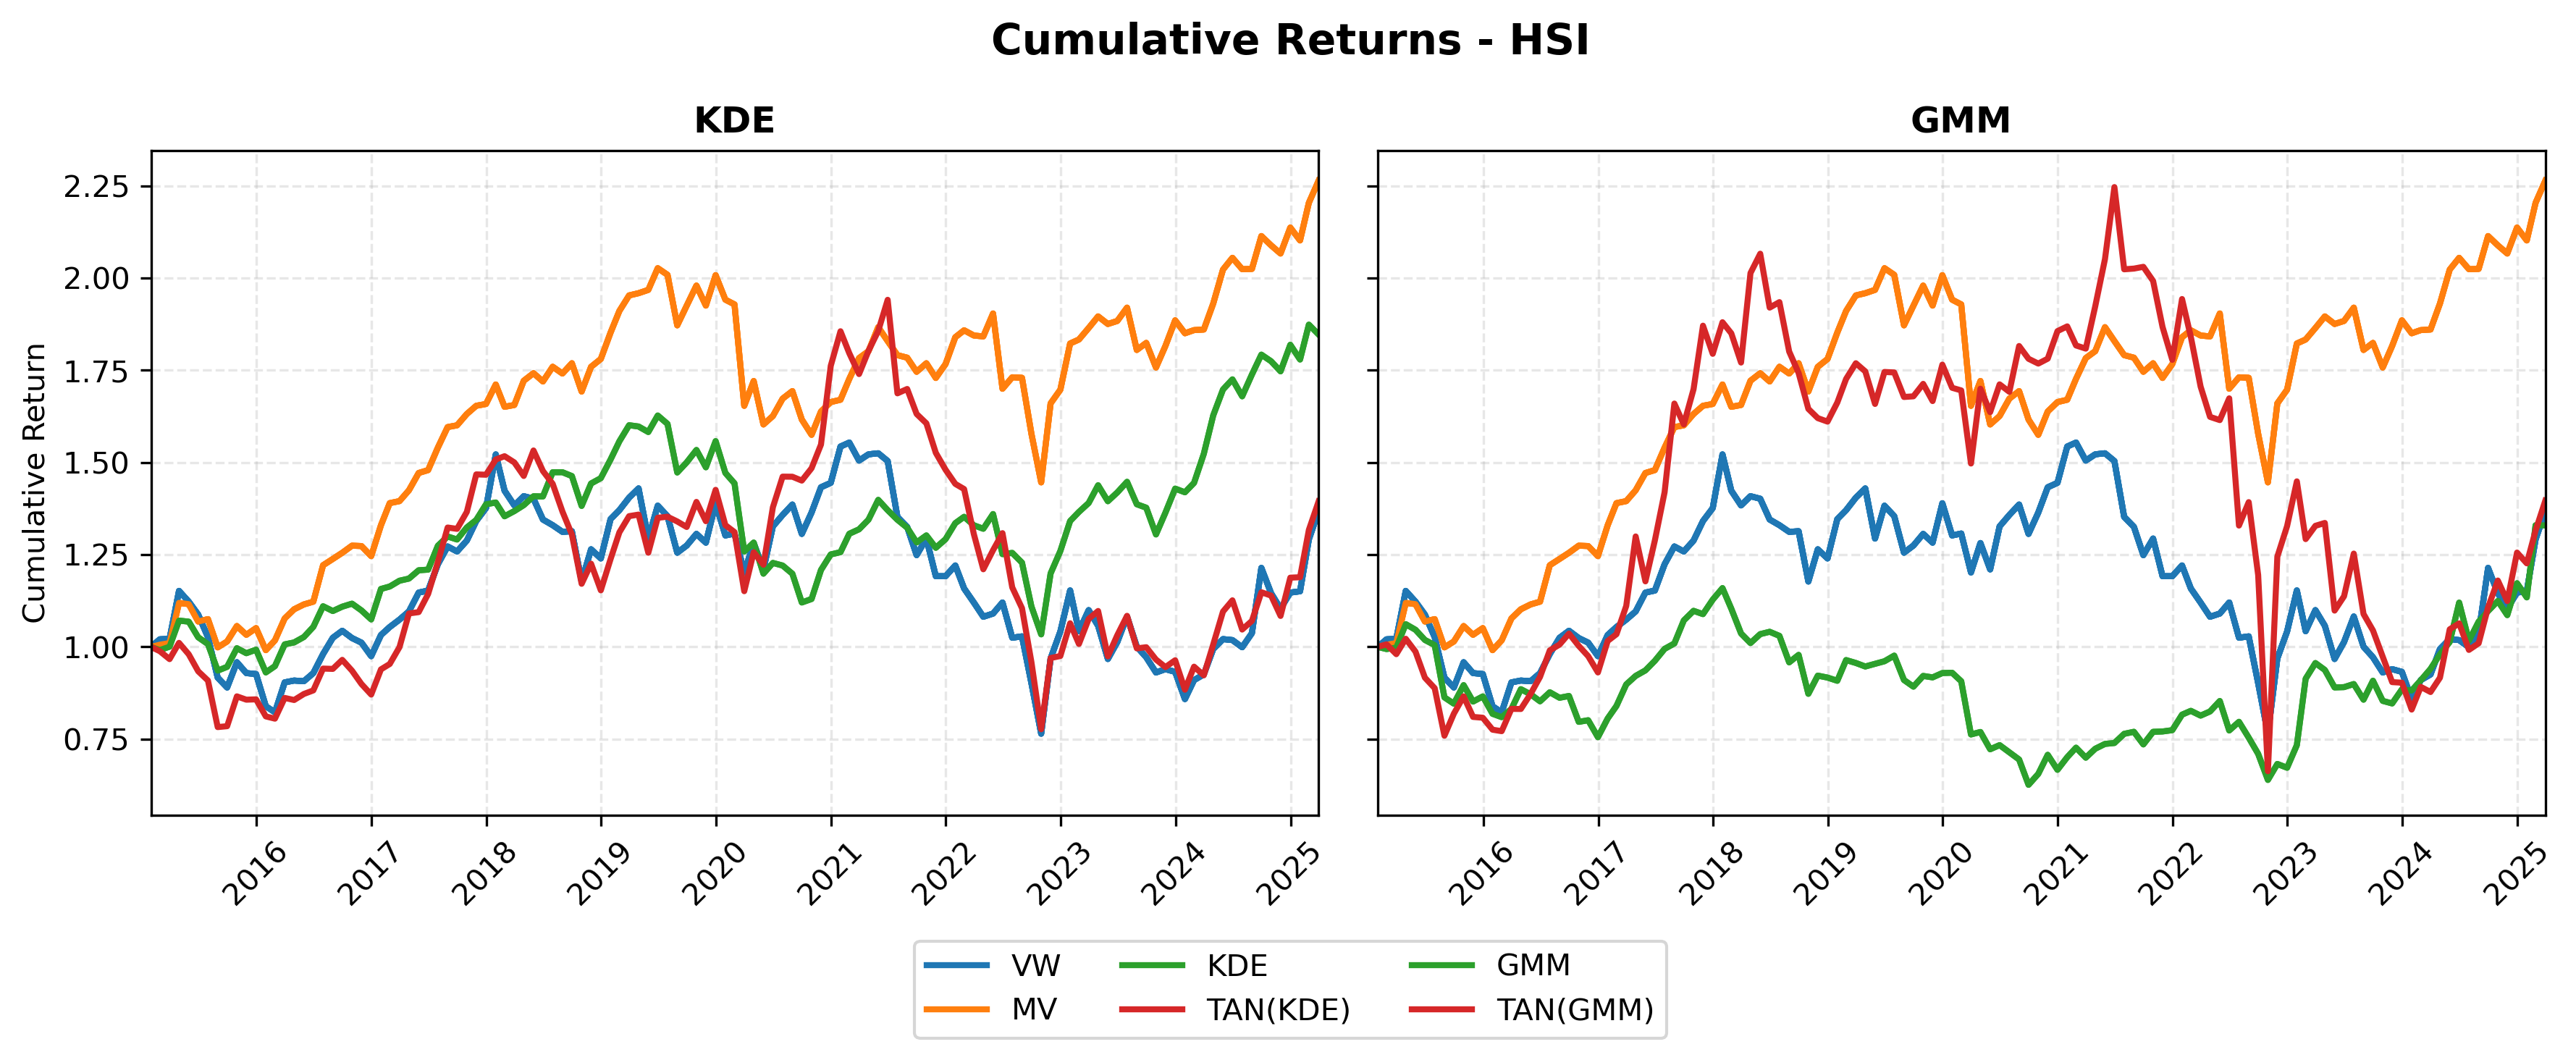
\includegraphics[width=\textwidth]{images/40_7.png}
  \end{minipage}
  \caption[Global best configuration - HSI - Cumulative returns]{Cumulative returns (Jan 2015-Mar 2025) of the best global configuration per strategy on the HSI index. Same layout as Figure \ref{fig:combined6}.}
  \label{fig:combined7}
  \end{center}
  \end{figure}

The GMM portfolio achieved decently low volatility, but at the cost of the lowest cumulative return. On the positive side, GMM did not suffer from the same cataclysmic drawdown of its tangency variant. The TAN(GMM) portfolio was the riskiest of all strategies, with the deepest downside.

\newpage
\begin{center}
  \textbf{S\&P500}
\end{center}
\begin{table}[H]
  \centering
  \begin{tabular}{l*{7}{S[table-format=1.4]}}
  \toprule
  & {$\mu$} & {$\sigma$} & {CR} & {SR} & {VaR} & {DD} & {\textbar DD\textbar} \\
  \midrule
  VW & 0.1373 & 0.1520 & 2.3288 & 0.8406 & 0.2313 & 0.2358 & 1.9167 \\
  MV & 0.0735 & {\bfseries 0.0953} & 0.9649 & 0.5650 & {\bfseries 0.1256} & 0.2380 & 1.8115 \\
  MAR & {\bfseries 0.2353} & 0.2505 & {\bfseries 5.2266} & {\bfseries 0.8490} & 0.3917 & 0.3695 & 2.2077 \\
  TAN & 0.1251 & 0.1591 & 1.9467 & 0.6802 & 0.2752 & 0.1986 & 1.8333 \\
  KDE & 0.0993 & 0.1205 & 1.4329 & 0.6573 & 0.1699 & 0.2484 & {\bfseries 1.7846} \\
  GMM & 0.0525 & 0.1964 & 0.3806 & 0.1754 & 0.2961 & 0.4608 & 6.1538 \\
  TAN(KDE) & 0.1236 & 0.1459 & 1.9678 & 0.7309 & 0.2351 & {\bfseries 0.1585} & 2.0833 \\
  TAN(GMM) & 0.1792 & 0.2021 & 3.4388 & 0.7928 & 0.2889 & 0.2532 & 2.0833 \\
  \bottomrule
\end{tabular}

  \caption[Global best configuration - All strategies - S\&P500]{Annualized performance of all portfolios (Jan 2015-Mar 2025), S\&P500 only. Averaged across all portfolio sizes. Same metrics as in Table \ref{tab:single1}.}
  \label{tab:single7}
\end{table}

\begin{figure}[H]
  \begin{center}
  \begin{minipage}{1\textwidth}
    \centering
    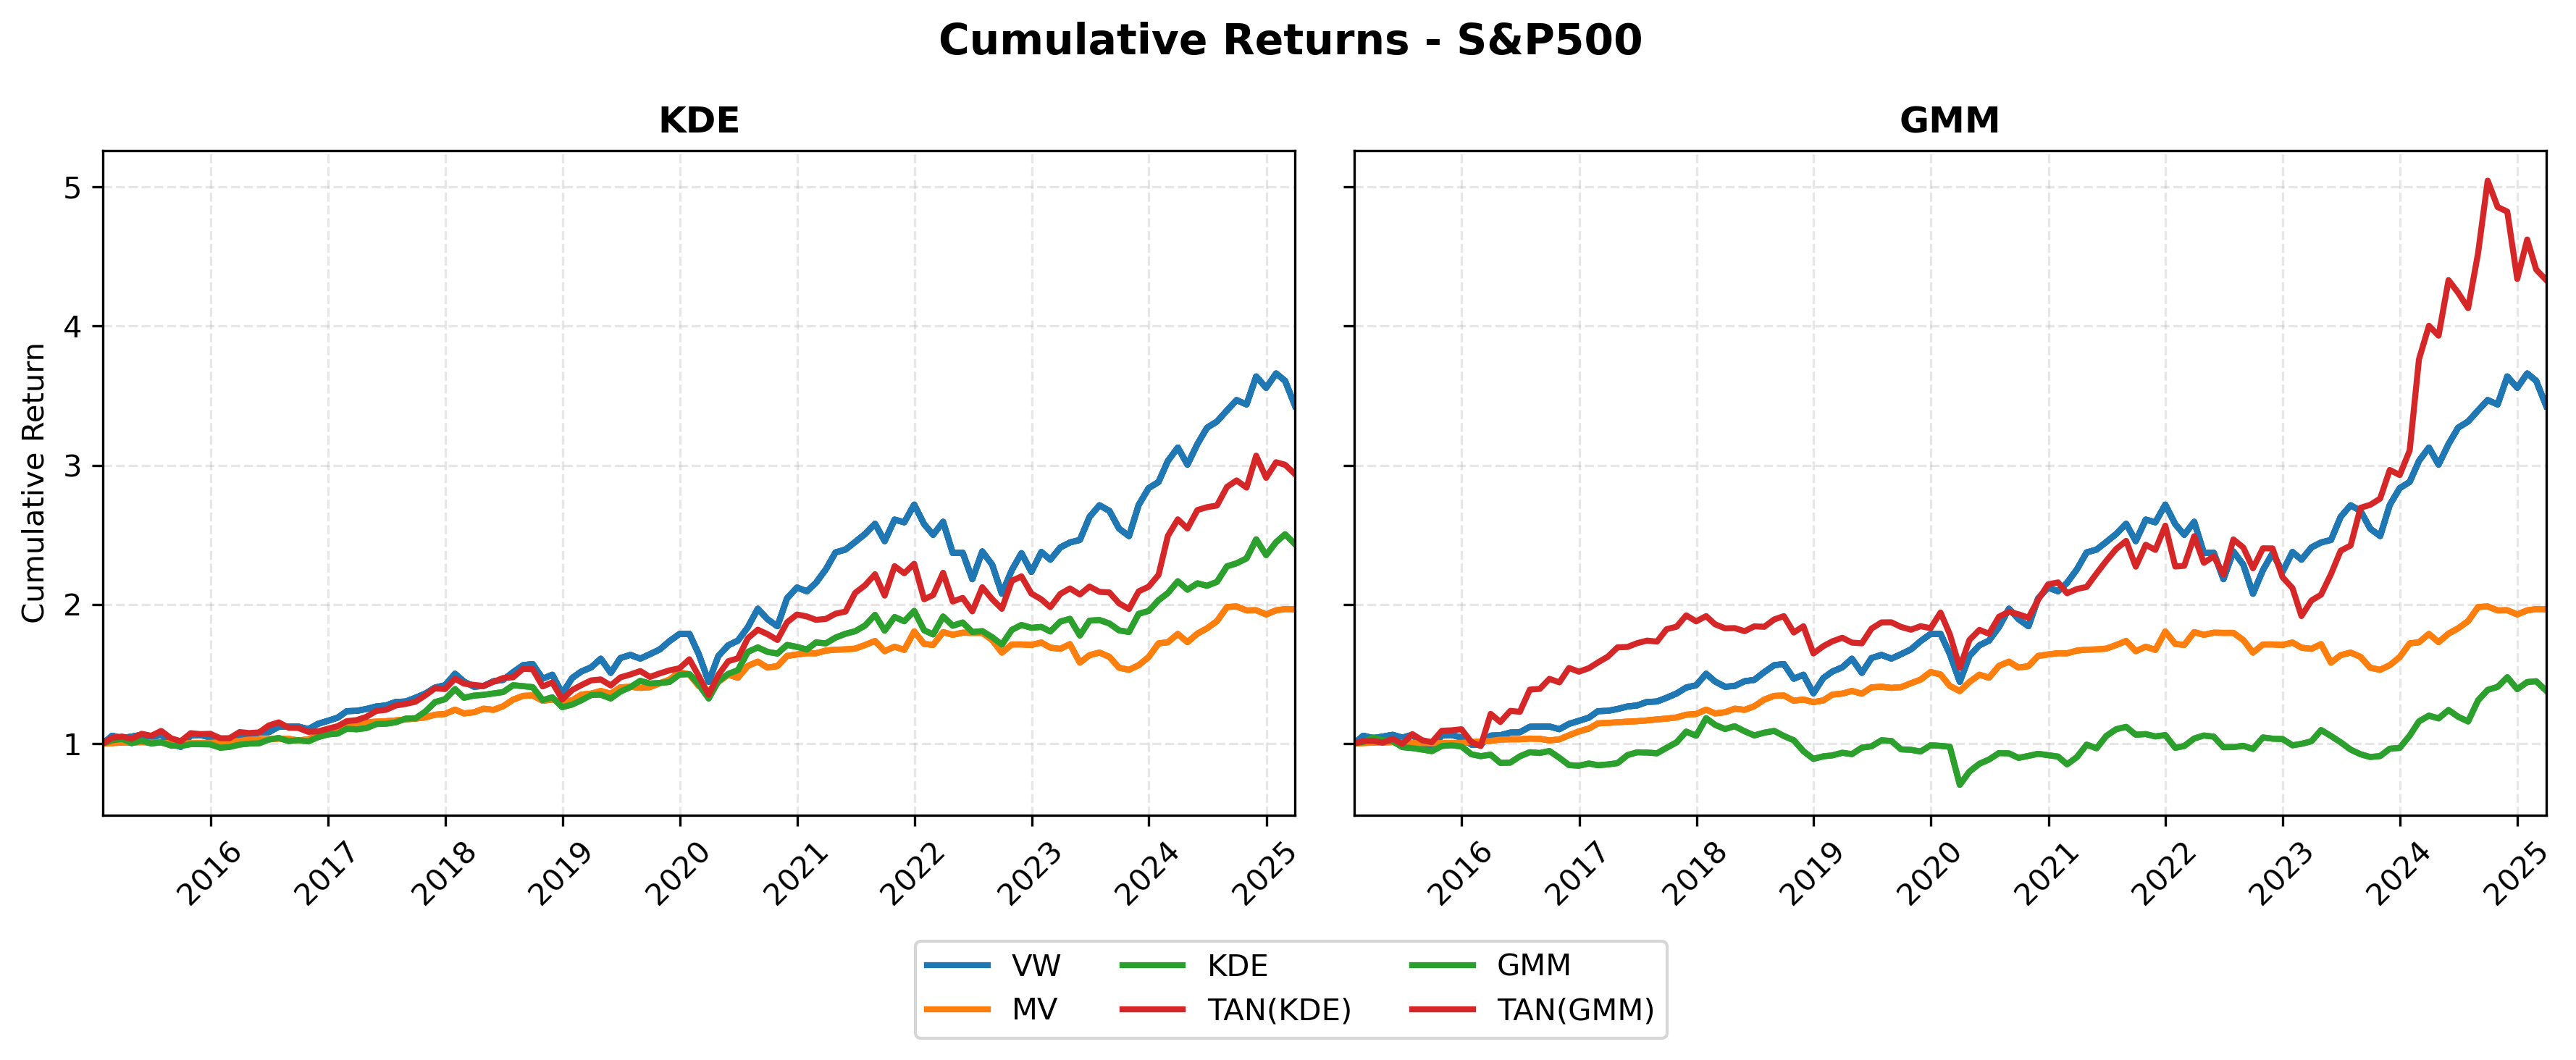
\includegraphics[width=\textwidth]{images/40_8.png}
  \end{minipage}
  \caption[Global best configuration - S\&P500 - Cumulative returns]{Cumulative returns (Jan 2015-Mar 2025) of the best global configuration per strategy on the S\&P500 index. Same layout as Figure \ref{fig:combined6}.}
  \label{fig:combined8}
  \end{center}
  \end{figure}

In the S\&P500, the VW portfolio delivered its best performance, with the second-best Sharpe Ratio and a competitive cumulative return. The MV portfolio again maintained the lowest volatility and $VaR$, although it did not lead in terms of drawdown length or depth.

The KDE portfolio performed modestly on most metrics, underdelivering in return and risk-adjusted terms. Its relative strength was in $|DD|$ and $VaR$, where it achieved the best and second-best results, respectively. In contrast, TAN(KDE) ranked among the best performers in cumulative return while offering a strong risk profile, including the shallowest drawdown of any portfolio in the S\&P, 7.9\% lower than the MV strategy.

The GMM portfolio proved to be the weakest performer in the S\&P500. It delivered the lowest cumulative return and Sharpe ratio of any strategy, while also suffering the highest volatility, worst VaR, and deepest drawdown. Its reliance on just six months of monthly data for nearly 500 assets likely exacerbates its instability, a point we revisit in Section \ref{sec:localoptima}. By comparison, the TAN(GMM) delivered a more moderate risk profile. Though its returns, volatility, and drawdown fail to entice when compared to other strategies.

\begin{center}
  \textbf{STOXX50}
\end{center}
\begin{table}[H]
  \centering
  \begin{tabular}{l*{7}{S[table-format=1.4]}}
  \toprule
  & {$\mu$} & {$\sigma$} & {CR} & {SR} & {VaR} & {DD} & {\textbar DD\textbar} \\
  \midrule
  VW & 0.1042 & 0.1687 & 1.3961 & 0.4724 & 0.2246 & 0.2562 & 1.9167 \\
  MV & 0.0858 & {\bfseries 0.1397} & 1.0869 & 0.4714 & {\bfseries 0.2078} & 0.3195 & 1.6077 \\
  MAR & {\bfseries 0.1343} & 0.2212 & 1.8032 & 0.5133 & 0.3443 & 0.4685 & 2.4692 \\
  TAN & 0.1253 & 0.1698 & 1.9021 & 0.5904 & 0.2420 & 0.2954 & 2.4167 \\
  KDE & 0.0751 & 0.1459 & 0.8709 & 0.3796 & 0.2168 & 0.3353 & 3.9500 \\
  GMM & 0.1017 & 0.2074 & 1.1508 & 0.3854 & 0.2844 & 0.3175 & 4.0192 \\
  TAN(KDE) & 0.1244 & 0.1636 & {\bfseries 1.9095} & {\bfseries 0.5905} & 0.2221 & {\bfseries 0.2482} & {\bfseries 1.2500} \\
  TAN(GMM) & 0.1136 & 0.1999 & 1.4643 & 0.4518 & 0.2944 & 0.2742 & 3.0833 \\
  \bottomrule
\end{tabular}

  \caption[Global best configuration - All strategies - STOXX50]{Annualized performance of all portfolios (Jan 2015-Mar 2025), STOXX50 only. Averaged across all portfolio sizes. Same metrics as in Table \ref{tab:single1}.}
  \label{tab:single8}
\end{table}

\begin{figure}[H]
  \begin{center}
  \begin{minipage}{1\textwidth}
    \centering
    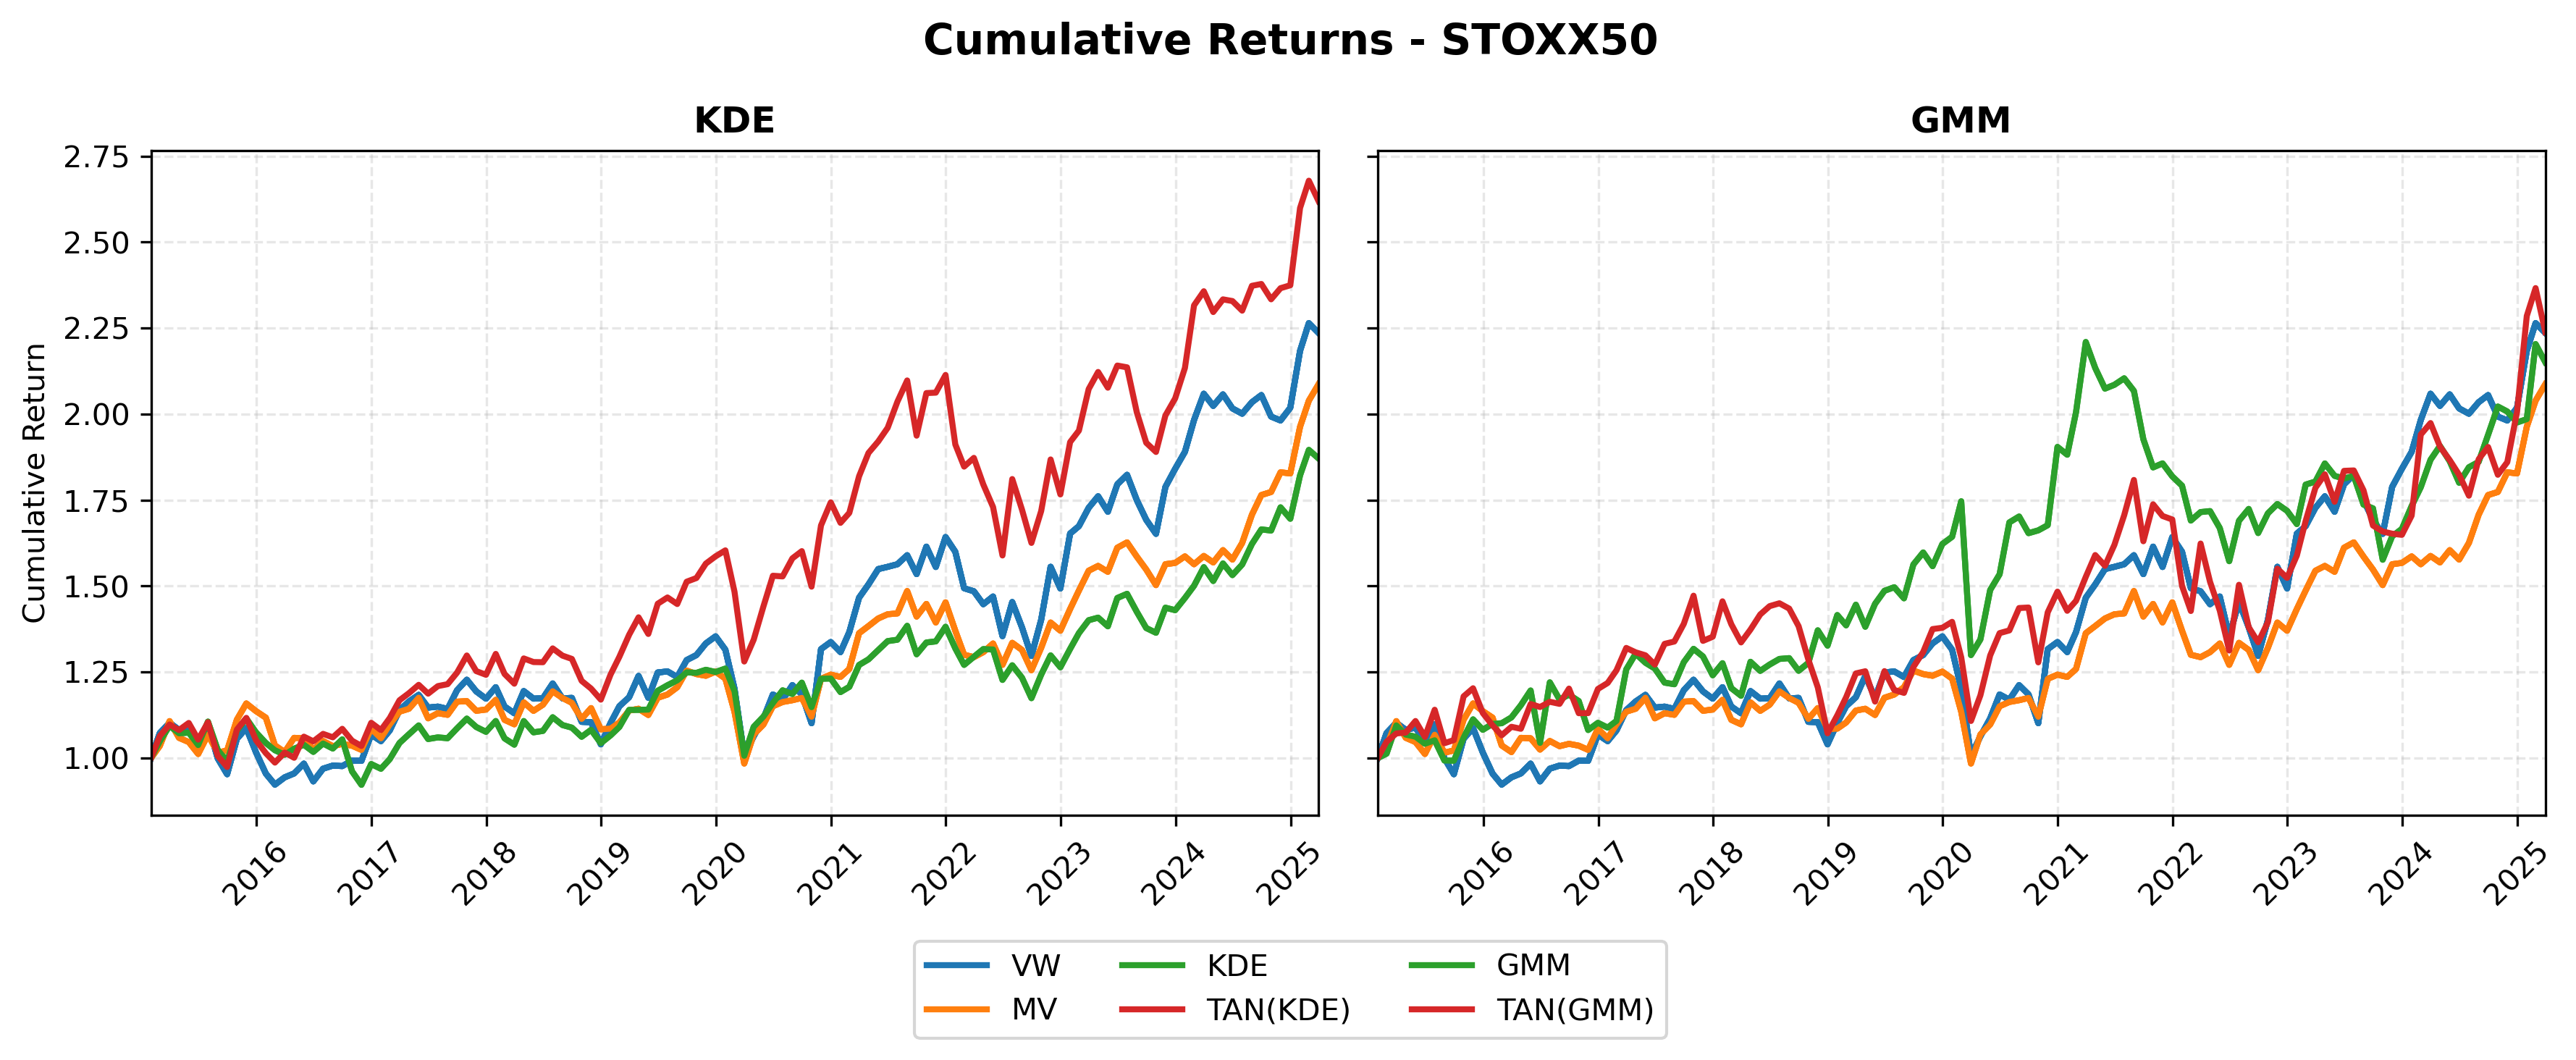
\includegraphics[width=\textwidth]{images/40_9.png}
  \end{minipage}
  \caption[Global best configuration - STOXX50 - Cumulative returns]{Cumulative returns (Jan 2015-Mar 2025) of the best global configuration per strategy on the STOXX50 index. Same layout as Figure \ref{fig:combined6}.}
  \label{fig:combined9}
  \end{center}
  \end{figure}

In the STOXX 50, the VW portfolio delivered middle-of-the-pack results across all metrics. At the same time, MV once again achieved the lowest volatility but also recorded a comparatively high drawdown. 

The KDE portfolio performed similarly to VW, with slightly lower volatility and a deeper and longer drawdown. The TAN(KDE) portfolio was the strongest overall performer, ranking first in cumulative and risk-adjusted returns and drawdown management. It also achieved the second-best $VaR$, second only to MV.

The standard GMM portfolio struggled, achieving one of the lowest Sharpe ratios and elevated volatility, although its maximum drawdown was marginally smaller than MV's. The TAN(GMM) variant proved more successful, essentially a higher volatility variant of VW. However, unlike KDE, its extra volatility did not translate into deeper drawdowns, which were among the shallowest, albeit with longer durations.

\subsection{Overview}
The preceding analysis aimed to compare the consistency and adaptability of various portfolio construction approaches to varying market regimes. The results underscore that while no single strategy dominates universally, certain approaches exhibit more reliable performance characteristics than others.

The VW portfolio demonstrates remarkable robustness, achieving the highest penalized Sharpe Ratio overall. This finding reinforces the challenge of consistently outperforming simple market-cap weighting when accounting for strategy stability across markets. The VW approach benefits from its simplicity and absence of estimation error, delivering competitive performance without the parameter sensitivity that affects more complex methods.

The MV portfolio also performs admirably, particularly in risk management, consistently delivering low volatility across most indices while maintaining competitive Sharpe Ratios. This highlights the enduring value of variance minimization as a portfolio construction technique, especially for risk-averse investors.

Among the density-based approaches, KDE portfolios show greater consistency than their GMM counterparts. The TAN(KDE) portfolio performs particularly well, achieving the second-highest raw Sharpe Ratio overall and demonstrating adaptability across indices. This suggests kernel density estimation provides a more stable foundation for portfolio optimization in diverse market conditions, likely due to its non-parametric nature and reduced sensitivity to outliers.

The GMM-based strategies exhibit the most variable performance across indices. While GMM achieved exceptional results in the S\&P500, its performance was inconsistent in other markets. When applied to sparse data, the anomalously high returns in the S\&P500 raise questions about model stability. This variability suggests that GMM approaches may be more sensitive to market-specific characteristics and data conditions, making them less reliable as globally portable strategies without careful calibration.

The index-specific analysis reveals how market structure influences strategy performance. In the highly concentrated HSI, MV significantly outperformed VW, while in the more diversified S\&P500, VW delivered exceptional results. While data-heavy density-based approaches can outperform traditional methods, they do not consistently dominate across all market environments. The VW and MV portfolios remain compelling due to their simplicity and reliability. For practitioners seeking to implement density-based approaches, KDE offers a more stable foundation than GMM, particularly when constructing tangency portfolios.

This section highlights the importance of rigor in strategy selection, especially for investors operating across multiple markets. The choice of optimal strategy and configuration should focus on specific characteristics of the target market, rather than the global performance metrics. In the following sections, we focus on the optimal configuration selection per index and attempt to provide heuristics for future practitioners.

\section{Local Configuration Optima}
\label{sec:localoptima}

Next, we explore how well the strategies perform when the best index-specific configuration is selected. We will once again employ the penalized Sharpe Ratio as our selection criterion for the optimal parameters. Additionally, in this section, we will display cumulative returns of subsampled configurations, if the optimum does not turn out to be to invest in the entirety of the index.

This analysis focuses on median cumulative returns as a measure of central tendency across multiple iterations. For the cumulative return plots, certain portfolios are displayed with an envelope representing the 5\% and 95\% quantiles of the cumulative return series for that configuration.

It's worth noting that it was this local analysis that lead us to identify a performance stability issue. The dominant configurations for MAR and KDE in the S\&P500 presented extremely high cumulative returns and a wide min-max quantile dispersion. With as few as six observations of monthly returns to determine weights for 450 assets, the ratio of observations-to-assets for these configurations was only 1.3\%. This over-performance, coupled with the data sparsity, led us to question the statistical validity of these results. Therefore, we elected to exclude all configurations with an observation-to-asset ratio below 10\% from all empirical analysis in this thesis. This decision is discussed in more detail in Section \ref{sec:limitations}.

\vspace{10mm}
\begin{table}[H]
  \centering
  \begin{table}[H]
  \centering
  \small
  \renewcommand{\arraystretch}{0.9}
  \setlength{\tabcolsep}{3pt}
  % preamble: \usepackage{tabularx,booktabs}
  %           \newcolumntype{Y}{>{\centering\arraybackslash}X}
  \begin{tabularx}{\textwidth}{llccccYYYYYYY}
  \toprule
    &  & \multicolumn{4}{c}{Configuration} & \multicolumn{7}{c}{Metrics} \\
  \cmidrule(lr){3-6} \cmidrule(lr){7-13}
    Index & Strategy & Reb. & Wnd. & Data & N & CR & SR & SR$_p$ & VaR & DD & \textbar DD\textbar & Disp. \\
  \midrule
    \multirow{8}{*}{\textbf{FTSE100}} & VW & monthly & 36 & monthly & 30 & 2.00 & 0.46 & 0.40 & \textbf{0.18} & 0.27 & 2.14 & \textbf{0.46} \\
     & MV & annual & 36 & monthly & 30 & 2.09 & 0.47 & 0.37 & 0.18 & 0.26 & 1.93 & 0.92 \\
     & MAR & annual & 6 & weekly & 30 & \textbf{2.69} & 0.53 & 0.35 & 0.29 & 0.41 & 3.13 & 2.66 \\
     & TAN & annual & 120 & monthly & 30 & 2.19 & 0.47 & 0.33 & 0.21 & 0.23 & 2.36 & 1.31 \\
     & KDE & annual & 36 & monthly & 30 & 2.38 & \textbf{0.59} & \textbf{0.43} & 0.18 & \textbf{0.20} & \textbf{1.90} & 1.46 \\
     & GMM & annual & 6 & monthly & 30 & 2.24 & 0.50 & 0.30 & 0.22 & 0.31 & 3.65 & 2.45 \\
     & TAN(KDE) & annual & 3 & weekly & 30 & 2.33 & 0.49 & 0.36 & 0.23 & 0.37 & 2.34 & 1.50 \\
     & TAN(GMM) & annual & 3 & weekly & 30 & 2.25 & 0.45 & 0.29 & 0.25 & 0.37 & 3.21 & 1.98 \\
  \midrule
    \multirow{8}{*}{\textbf{HSI}} & VW & annual & 60 & daily & 20 & 1.55 & 0.24 & 0.16 & 0.30 & 0.41 & 5.08 & 0.76 \\
     & MV & monthly & 3 & daily & 30 & 2.43 & \textbf{0.62} & \textbf{0.56} & \textbf{0.20} & \textbf{0.28} & 3.99 & \textbf{0.50} \\
     & MAR & annual & 12 & daily & 30 & 2.17 & 0.40 & 0.31 & 0.31 & 0.42 & 4.94 & 1.11 \\
     & TAN & monthly & 12 & daily & 30 & \textbf{2.87} & 0.54 & 0.42 & 0.32 & 0.39 & 3.23 & 2.16 \\
     & KDE & monthly & 3 & daily & 30 & 2.25 & 0.53 & 0.47 & 0.22 & 0.30 & 4.14 & 0.54 \\
     & GMM & monthly & 6 & daily & 30 & 1.96 & 0.38 & 0.25 & 0.26 & 0.43 & 4.58 & 1.42 \\
     & TAN(KDE) & monthly & 12 & daily & 30 & 2.80 & 0.54 & 0.41 & 0.31 & 0.39 & 3.20 & 2.30 \\
     & TAN(GMM) & monthly & 6 & weekly & 30 & 2.26 & 0.44 & 0.31 & 0.29 & 0.37 & \textbf{3.13} & 1.79 \\
  \midrule
    \multirow{8}{*}{\textbf{S\&P500}} & VW & annual & 120 & monthly & 450 & 3.40 & 0.86 & 0.85 & 0.23 & 0.23 & \textbf{1.50} & \textbf{0.07} \\
     & MV & monthly & 3 & daily & 100 & 2.49 & 0.67 & 0.57 & \textbf{0.18} & 0.26 & 1.89 & 1.08 \\
     & MAR & annual & 120 & monthly & 450 & \textbf{5.55} & 0.95 & 0.88 & 0.26 & 0.33 & 1.95 & 1.95 \\
     & TAN & annual & 120 & monthly & 450 & 4.26 & \textbf{0.99} & \textbf{0.89} & 0.24 & 0.19 & 1.85 & 3.04 \\
     & KDE & monthly & 120 & monthly & 450 & 3.73 & 0.83 & 0.68 & 0.24 & 0.19 & 1.79 & 2.86 \\
     & GMM & monthly & 120 & monthly & 450 & 4.05 & 0.83 & 0.68 & 0.23 & 0.22 & 2.05 & 2.85 \\
     & TAN(KDE) & annual & 120 & monthly & 450 & 3.56 & 0.90 & 0.85 & 0.23 & 0.20 & 1.76 & 0.60 \\
     & TAN(GMM) & monthly & 120 & monthly & 450 & 4.84 & 0.95 & 0.82 & 0.25 & \textbf{0.19} & 1.75 & 3.23 \\
  \midrule
    \multirow{8}{*}{\textbf{STOXX50}} & VW & annual & 3 & monthly & 30 & 2.43 & 0.49 & 0.45 & \textbf{0.23} & \textbf{0.25} & 1.71 & \textbf{0.45} \\
     & MV & annual & 60 & daily & 30 & 3.02 & \textbf{0.67} & \textbf{0.58} & 0.24 & 0.33 & 1.70 & 1.19 \\
     & MAR & annual & 12 & daily & 30 & \textbf{3.23} & 0.63 & 0.51 & 0.31 & 0.40 & 2.06 & 2.53 \\
     & TAN & annual & 12 & daily & 30 & 2.94 & 0.57 & 0.45 & 0.30 & 0.39 & 2.39 & 2.02 \\
     & KDE & annual & 6 & daily & 30 & 2.51 & 0.55 & 0.50 & 0.23 & 0.34 & \textbf{1.63} & 0.60 \\
     & GMM & annual & 36 & monthly & 30 & 2.96 & 0.57 & 0.41 & 0.25 & 0.26 & 2.35 & 2.41 \\
     & TAN(KDE) & annual & 36 & monthly & 30 & 3.00 & 0.57 & 0.48 & 0.25 & 0.26 & 1.92 & 1.29 \\
     & TAN(GMM) & annual & 6 & weekly & 20 & 2.85 & 0.52 & 0.38 & 0.33 & 0.37 & 2.61 & 2.49 \\
  \bottomrule
  \end{tabularx}
\end{table}

  \caption[All optimal configurations]{Optimal configuration and end-of-period performance for each strategy by index. For each index and strategy, we report rebalancing frequency (Reb.), lookback window in months (Wnd.), data frequency (Data), and the number of assets in the portfolio (N). Performance metrics: cumulative return (CR), Sharpe ratio (SR), penalized Sharpe ratio (SR$_p$), terminal cumulative return dispersion (Disp.), maximum drawdown (DD), drawdown duration (|DD|), and 95\% Value-at-Risk (VaR); metrics are computed over the 2015-2025 sample. Within each index block, boldface highlights the best value in that column across strategies.}

  \label{tab:single9}
\end{table}

\newpage
We observe that the optimal configurations for MAR consistently generate the highest median cumulative returns (above 5.5 in the S\&P500). This outperformance, however, comes with substantially higher dispersion, often at or above 2.5. For context, the dispersion values for VW typically remain below 0.5, while MV portfolios range between 0.5 and 1.2. Values above 2.0 suggest a comparatively low strategy stability.

KDE portfolios consistently present a trade-off across markets. They achieve lower dispersion than their MAR counterparts (45-75\% improvement) in all markets but the S\&P500 (45\% increase). However, this stability frequently comes at the cost of lower absolute returns. While KDE sometimes achieves higher Sharpe ratios than MAR, particularly in smaller or less efficient markets, it consistently trails in cumulative returns.

\vspace{5mm}
\begin{figure}[H]
  \begin{center}
  \begin{minipage}{1\textwidth}
    \centering
    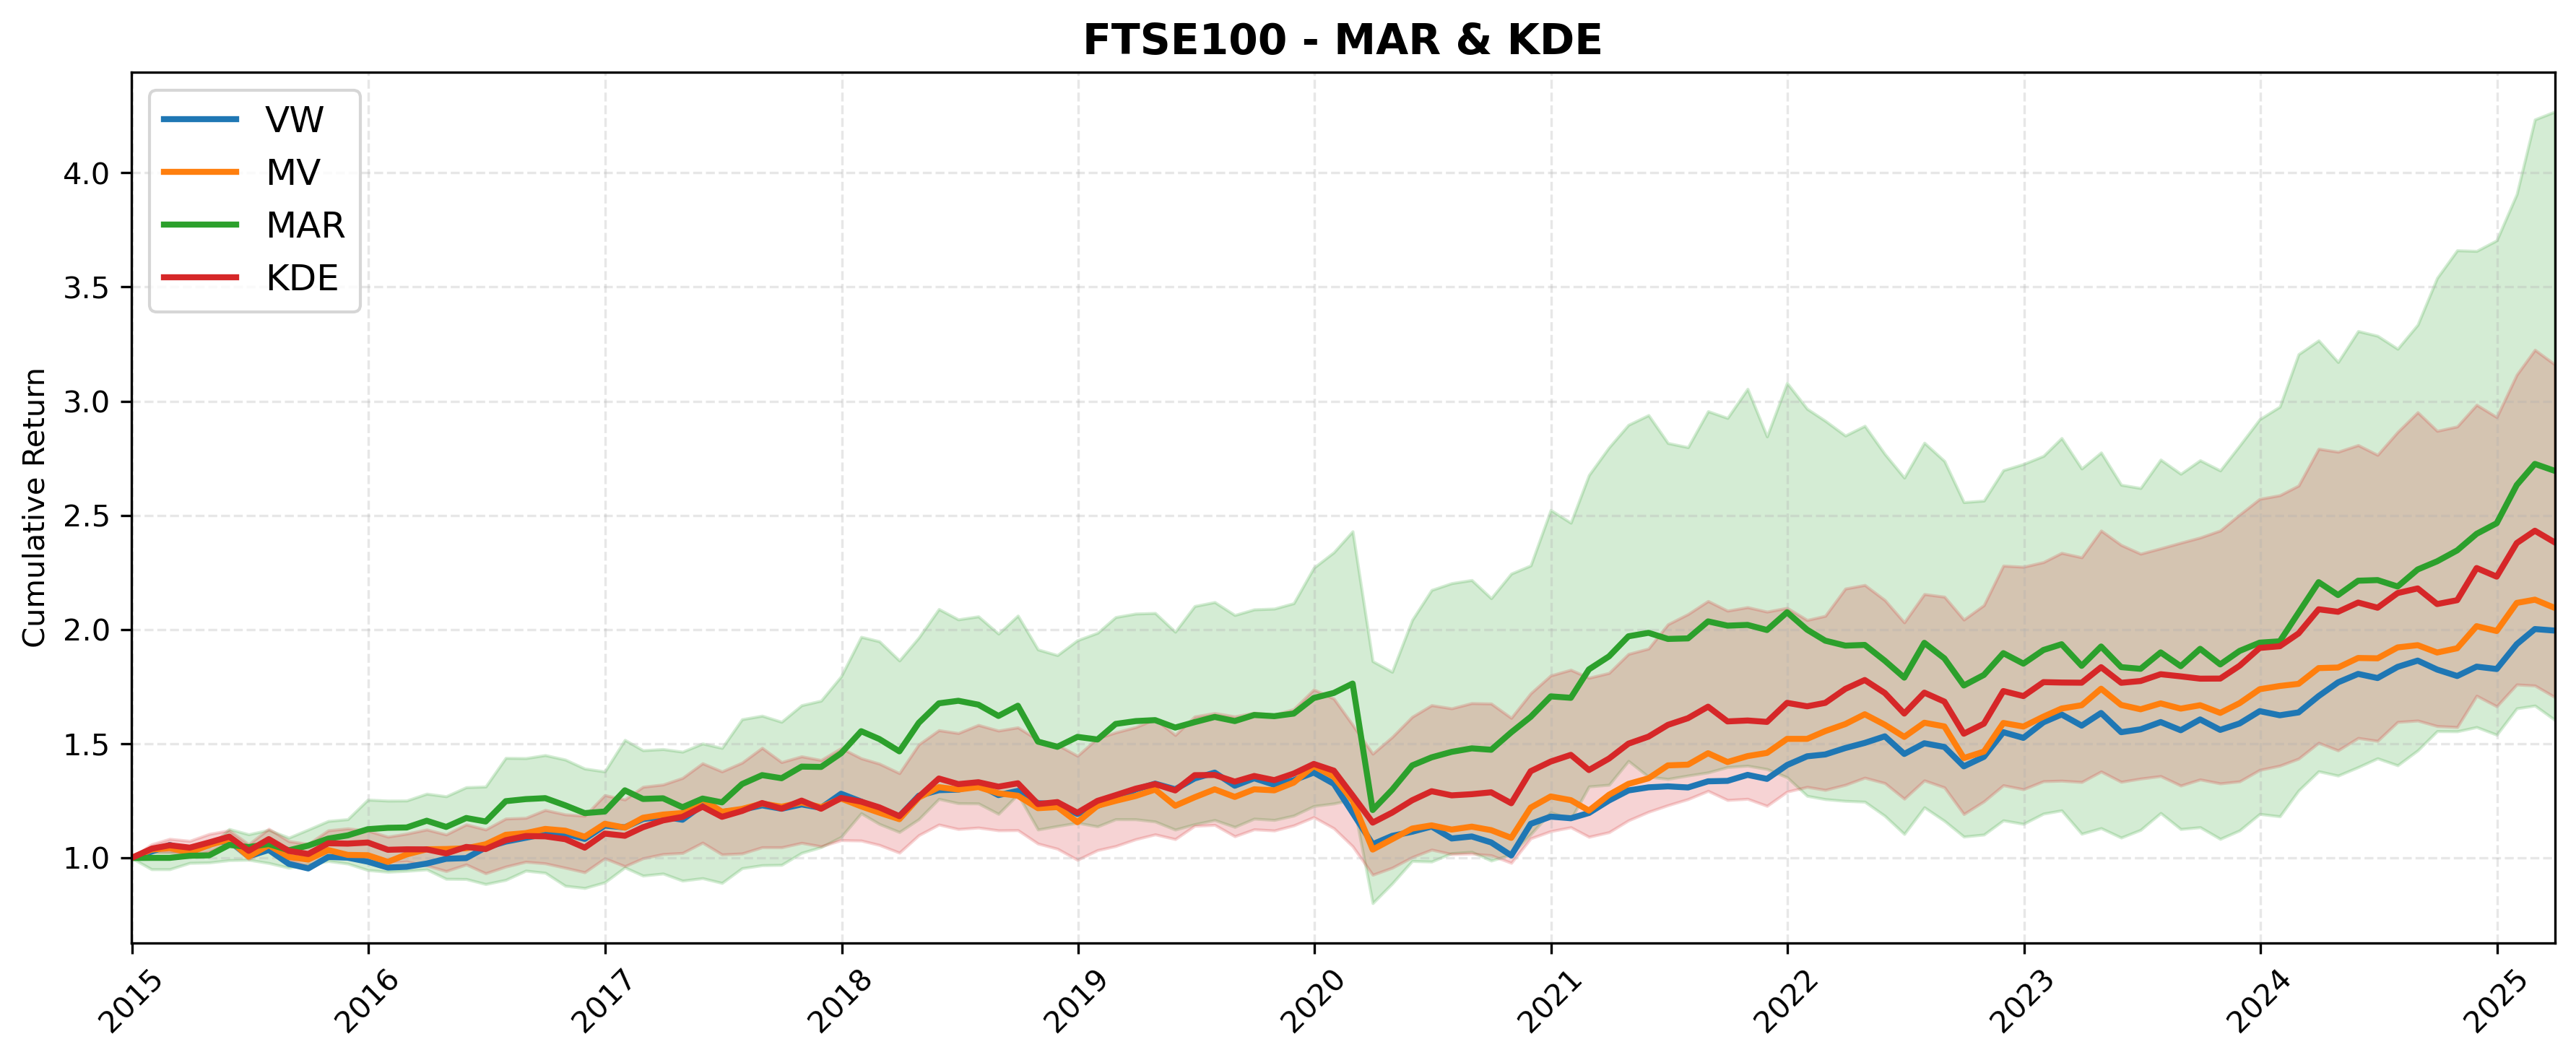
\includegraphics[width=\textwidth]{images/40_10.png}
  \end{minipage}
  \caption[Local best configuration - FTSE100 - Cumulative returns]{Cumulative returns (Jan 2015-Mar 2025) on the FTSE100 index of the locally optimal configuration for each strategy, selected by the highest penalized Sharpe ratio. VW (blue) and MV (orange) show the pointwise median of all cumulative-return paths; MAR (green) and KDE (red) additionally display shaded envelopes spanning the 5th-95th percentiles at each date. All series are normalized to 1.0 at the start date.}
  \label{fig:combined10}
  \end{center}
  \end{figure}

The performance of GMM portfolios also lacks consistency. While occasionally delivering strong performance, GMM typically exhibits high dispersion relative to returns, often matching or exceeding MAR's already elevated dispersion levels. More concerning is GMM's performance variability across different market environments, delivering competitive returns in some markets while significantly underperforming in others.

\begin{figure}[H]
  \begin{center}
  \begin{minipage}{1\textwidth}
    \centering
    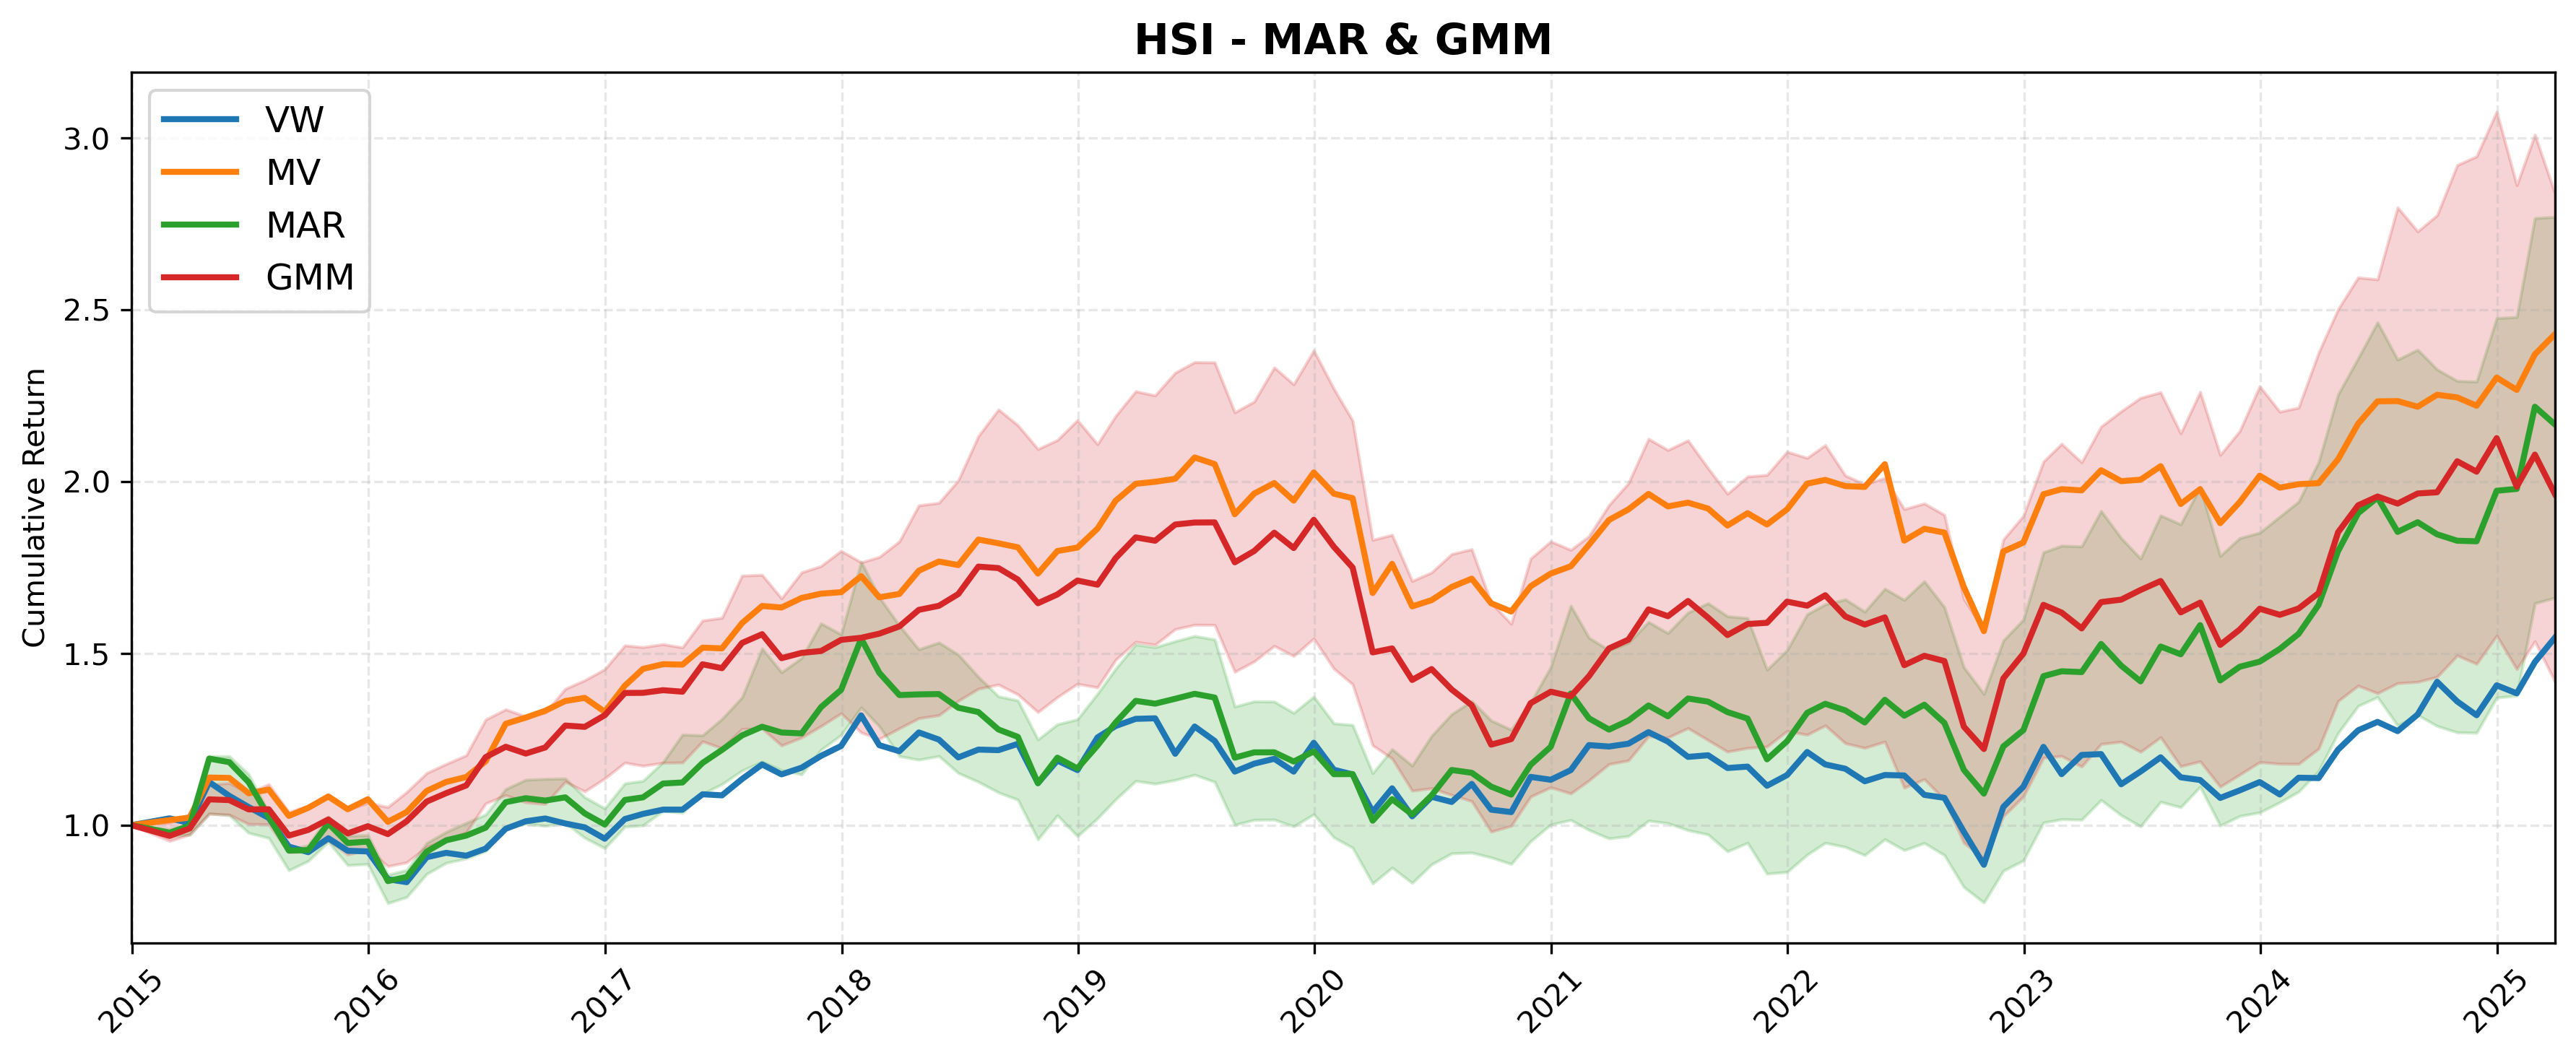
\includegraphics[width=\textwidth]{images/40_11.png}
  \end{minipage}
  \caption[Local best configuration - HSI - Cumulative returns]{Cumulative returns (Jan 2015-Mar 2025) on the HSI index of the locally optimal configuration for each strategy, selected by the highest penalized Sharpe ratio. Identical layout to Figure \ref{fig:combined10}, with the exception that the GMM portfolio (red) is shown instead of KDE.}
  \label{fig:combined11}
  \end{center}
  \end{figure}

KDE shows promise in tangency portfolio construction. TAN(KDE) demonstrates competitive performance with traditional TAN portfolios in terms of the Sharpe ratio, while typically offering lower dispersion. Notably, TAN(KDE) achieves an extremely low comparative dispersion in the S\&P500 of 0.602, lower than that of the MV portfolio. TAN(GMM) shows high return potential but continues to exhibit the highest dispersion values among all strategies, undermining its practical implementation value.

\vspace{5mm}
\begin{figure}[H]
  \begin{center}
  \begin{minipage}{1\textwidth}
    \centering
    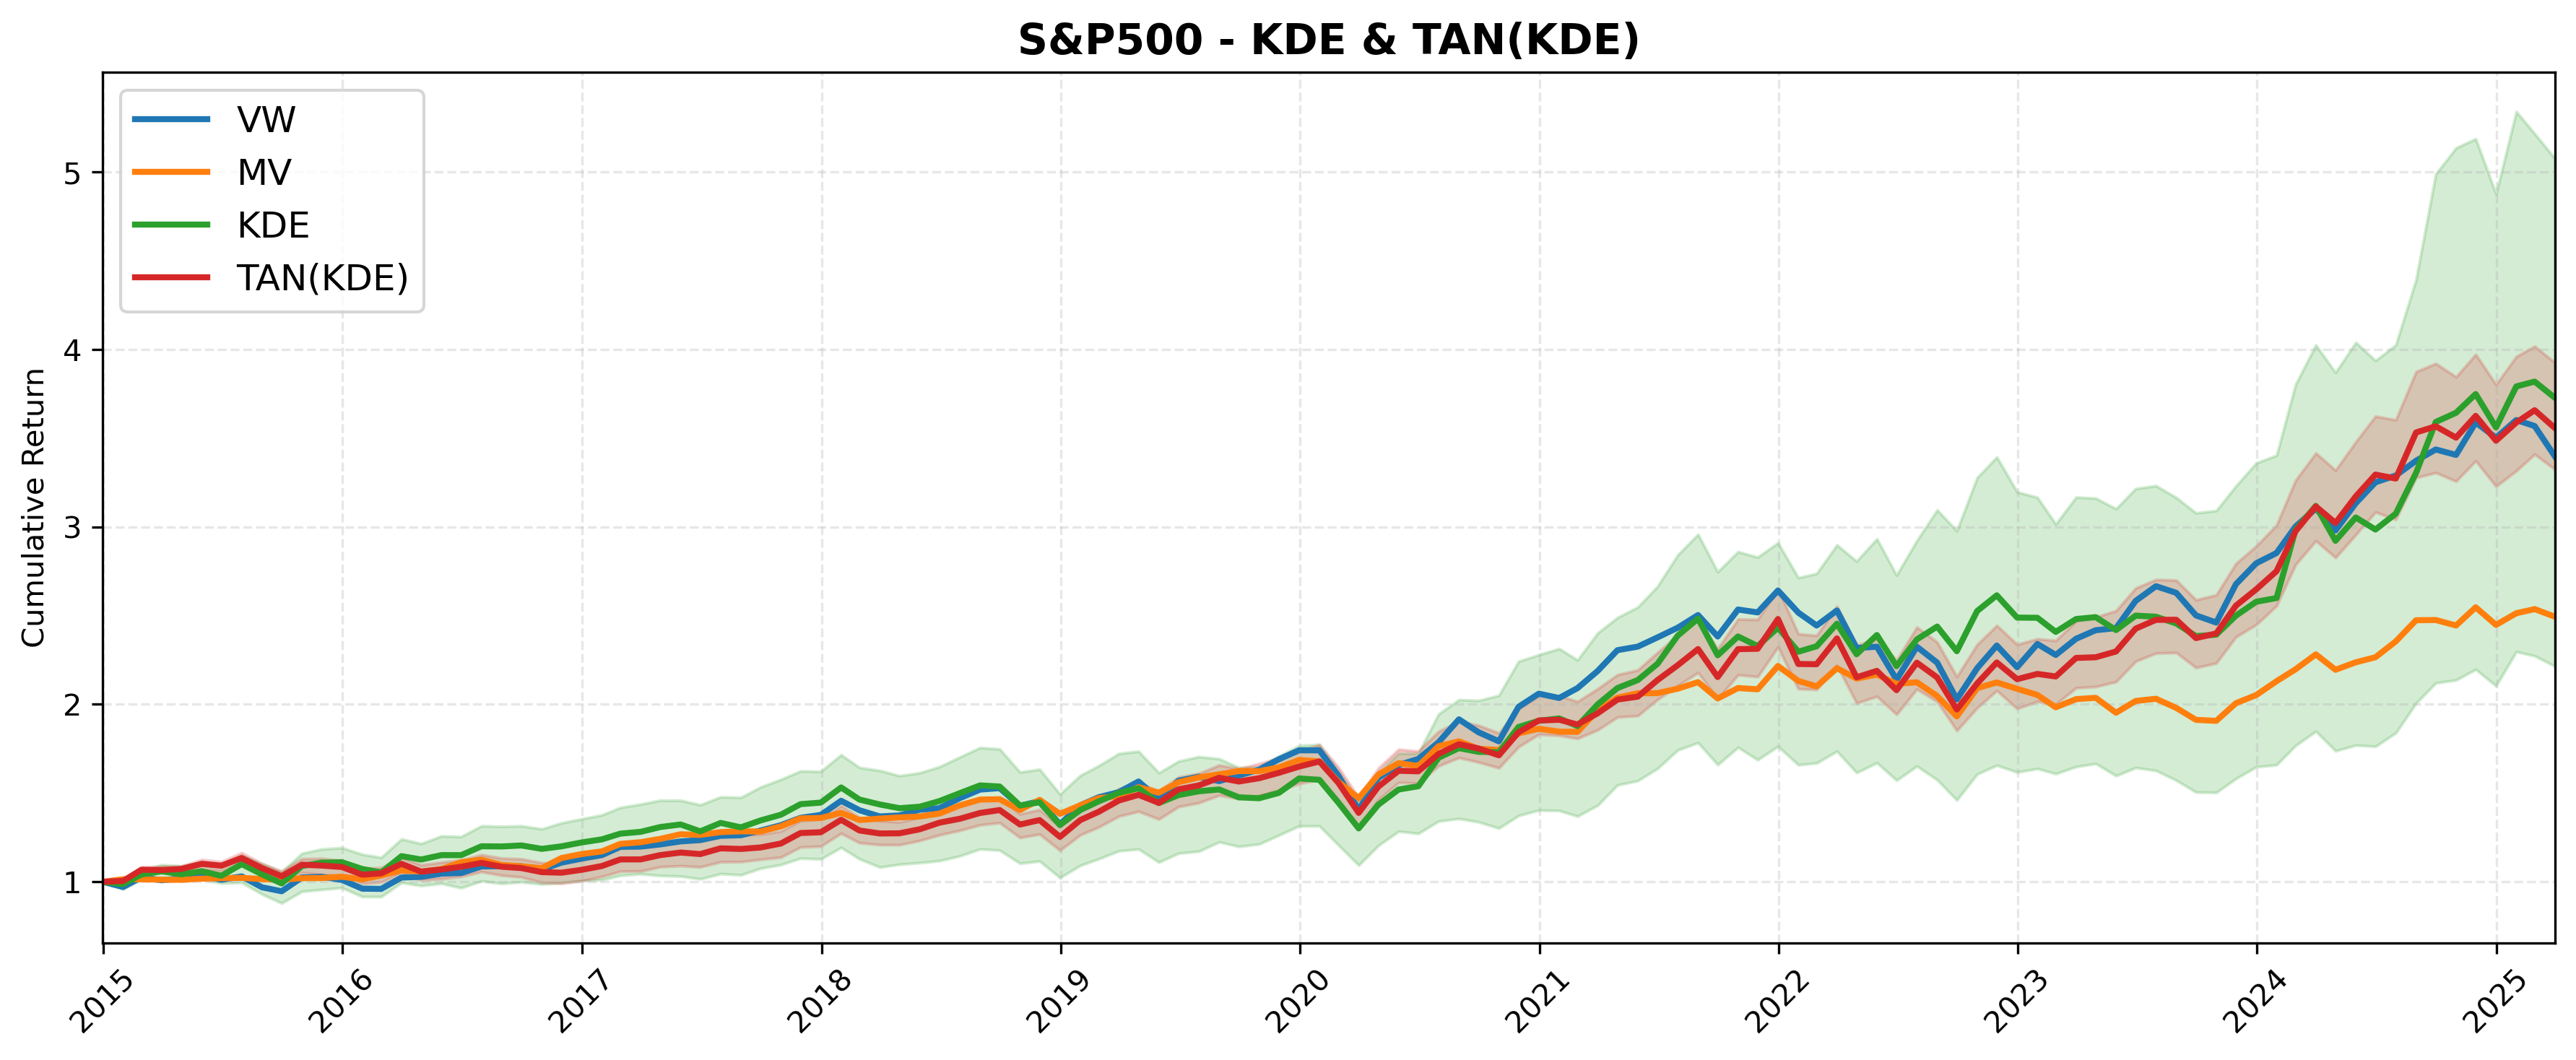
\includegraphics[width=\textwidth]{images/40_12.png}
  \end{minipage}
  \caption[Local best configuration - S\&P500 - Cumulative returns]{Cumulative returns (Jan 2015-Mar 2025) on the S\&P500 index of the locally optimal configuration for each strategy, selected by the highest penalized Sharpe ratio. Identical layout to Figure \ref{fig:combined10}, with the exception that the KDE portfolio (green) is shown instead of MAR, TAN(KDE) (red) instead of KDE.}
  \label{fig:combined12}
  \end{center}
  \end{figure}

The variations in configuration are partly responsible for the performance differences. KDE portfolios favor shorter lookback windows in smaller markets but require longer ones in the S\&P500, likely due to data demands in larger universes. GMM portfolios prefer intermediate windows in some markets and longer ones in others. The relationships between configurations and performance will be further examined in subsequent sections.

Maximum drawdown metrics reveal a more nuanced picture than initially apparent. In several instances, density-based approaches demonstrate superior drawdown protection compared to traditional portfolios. In the S\&P500, TAN(KDE) achieves a maximum drawdown of 20\%, lower than the MV portfolio's 26\%. Similarly, in the FTSE100, KDE records the lowest and shortest maximum drawdown among all strategies at 20\%, significantly outperforming both MAR (41\%) and MV (26\%). This pattern extends to Value-at-Risk measures, where KDE frequently records the lowest or second-lowest VaR figures across indices. The above demonstrates that KDE-based approaches offer enticing downside risk management while maintaining competitive returns.

KDE also demonstrates enhanced estimation stability compared to MAR and more consistent performance across markets than GMM. The advantage is most visible in tangency portfolios: TAN(KDE) matches or exceeds the returns of the traditional TAN while achieving significantly lower dispersion. This stability advantage persists across different market environments, suggesting that non-parametric density estimation adapts to heterogeneous return distributions well.

The rankings in Table \ref{tab:married1} crystallize this result. KDE now tops the overall table, finishing first in four of seven metrics and never worse than third; MV and TAN(KDE) share second place, while both GMM variants are relegated to the bottom of the rankings. In summary, once we equalise scale across markets, KDE emerges as the most consistently attractive strategy, with MV and TAN(KDE) close behind.

\vspace{10mm}
\begin{table}[H]
  \centering
  \begin{tabular}{l|c|*{7}{S[table-format=1.4]}}
  \toprule
  & {Avg. Rank} & {CR} & {SR} & {SR$_p$} & {VaR} & {DD} & {\textbar DD\textbar} & {Disp.} \\
  \midrule
  VW & {4th} & {8th} & {8th} & {6th} & {3rd} & {3rd} & {3rd} & {{\bfseries 1st}} \\
  MV & {{\textit{2nd}}} & {7th} & {5th} & {3rd} & {{\bfseries 1st}} & {2nd} & {4th} & {2nd} \\
  MAR & {6th} & {{\bfseries 1st}} & {{\bfseries 1st}} & {4th} & {8th} & {8th} & {7th} & {5th} \\
  TAN & {5th} & {2nd} & {3rd} & {5th} & {6th} & {6th} & {5th} & {6th} \\
  KDE & {{\bfseries 1st}} & {6th} & {2nd} & {{\bfseries 1st}} & {2nd} & {{\bfseries 1st}} & {{\bfseries 1st}} & {3rd} \\
  GMM & {7th} & {5th} & {6th} & {8th} & {4th} & {5th} & {8th} & {7th} \\
  TAN(KDE) & {{\textit{2nd}}} & {3rd} & {4th} & {2nd} & {5th} & {4th} & {2nd} & {4th} \\
  TAN(GMM) & {8th} & {4th} & {7th} & {7th} & {7th} & {7th} & {6th} & {8th} \\
  \bottomrule
\end{tabular}

  \caption[Optimal strategy ranking]{Relative performance of each strategy after normalising metrics within every index, averaging the normalised scores across the indices, and converting these averages to ordinal ranks (1=best). "Avg.Rank" is the arithmetic mean of the seven column ranks; the overall winner in each column is bold; contested rankings are italicised. Metric definitions are identical to Table \ref{tab:single9}.}
  \label{tab:married1}
\end{table}

\newpage
\section{Where \& Why Do Density-Based Strategies Win?}
% \clearpage
After filtering for stability (observation-to-asset ratio $\geq 10$\%), we assess the 828 remaining portfolio configurations per index. The heat maps in this section compare the differences in $SR_{p}$ or $DD$ between a selected portfolio type and a benchmark, for a given set of configurations. Blue always represents a positive difference (higher $SR_{p}$, lower $DD$), and red - a negative one. 
\vspace{10mm}
\begin{table}[H]
  \centering
  \begin{table}[H]
  \centering
  \setlength{\tabcolsep}{4pt}
  \renewcommand{\arraystretch}{1.0}
  \begin{tabular}{c|l|*{7}{S[table-format=3.2]}}
    Metric & Comparison & \multicolumn{1}{c}{$P(\delta^+)$} & \multicolumn{1}{c}{$E[\delta]$} & \multicolumn{1}{c}{$E[\delta^+]$} & \multicolumn{1}{c}{$E[\delta^-]$} & \multicolumn{1}{c}{$\max(\delta^+)$} & \multicolumn{1}{c}{$\min(\delta^-)$} \\
    \midrule
    \multirow{8}{*}{\textbf{SR$_p$}} & KDE - VW & 0.18 & -0.09 & 0.09 & -0.13 & 0.42 & -0.54 \\
    & KDE - MAR & 0.59 & 0.03 & 0.13 & -0.10 & 0.53 & -0.50 \\
    & TAN(KDE) - VW & 0.20 & -0.08 & 0.08 & -0.12 & 0.40 & -0.49 \\
    & TAN(KDE) - TAN & 0.83 & 0.02 & 0.03 & -0.02 & 0.20 & -0.16 \\
    \cmidrule[0.4pt]{2-2}
    & GMM - VW & 0.07 & -0.21 & 0.08 & -0.23 & 0.34 & -0.94 \\
    & GMM - MAR & 0.33 & -0.08 & 0.09 & -0.16 & 0.43 & -0.75 \\
    & TAN(GMM) - VW & 0.09 & -0.19 & 0.11 & -0.22 & 0.52 & -0.85 \\
    & TAN(GMM) - TAN & 0.15 & -0.09 & 0.03 & -0.11 & 0.26 & -0.68 \\
    \midrule
    \multirow{4}{*}{\textbf{DD}} & KDE - MV & 0.46 & -0.00 & 0.03 & -0.03 & 0.17 & -0.20 \\
    & TAN(KDE) - MV & 0.25 & -0.03 & 0.05 & -0.06 & 0.22 & -0.26 \\
    \cmidrule[0.4pt]{2-2}
    & GMM - MV & 0.07 & -0.07 & 0.03 & -0.07 & 0.17 & -0.34 \\
    & TAN(GMM) - MV & 0.09 & -0.09 & 0.04 & -0.10 & 0.18 & -0.34 \\
  \end{tabular}
\end{table}

  \caption[Metric comparison across all configurations]{Summary statistics for the performance difference $\delta$ between each strategy and its benchmark, across all stable window-rebalancing configurations. Two metrics are shown: inverted maximum drawdown (DD) and penalized Sharpe ratio (SR$_p$). For each Metric-Comparison pair, $P(\delta^+)$ is the proportion with positive $\delta$ (i.e.\ strategy improves over the benchmark), $E[\delta]$ is the mean increase, $E[\delta^+]$ and $E[\delta^-]$ are the mean positive and negative deviations, and $\max(\delta^+)$, $\min(\delta^-)$ give the largest increase and largest shortfall, respectively. 828 configurations per portfolio pair are compared.}
  \label{tab:single10}
\end{table}

Table \ref{tab:single10} is an aggregate of all stable configuration comparisons. The heatmap grids that follow, however, present this information per index, hence the slightly different ranges of values in Figures \ref{fig:combined13} to \ref{fig:combined17}.

\begin{figure}[H]
  \begin{center}
  \begin{minipage}{1\textwidth}
    \centering
    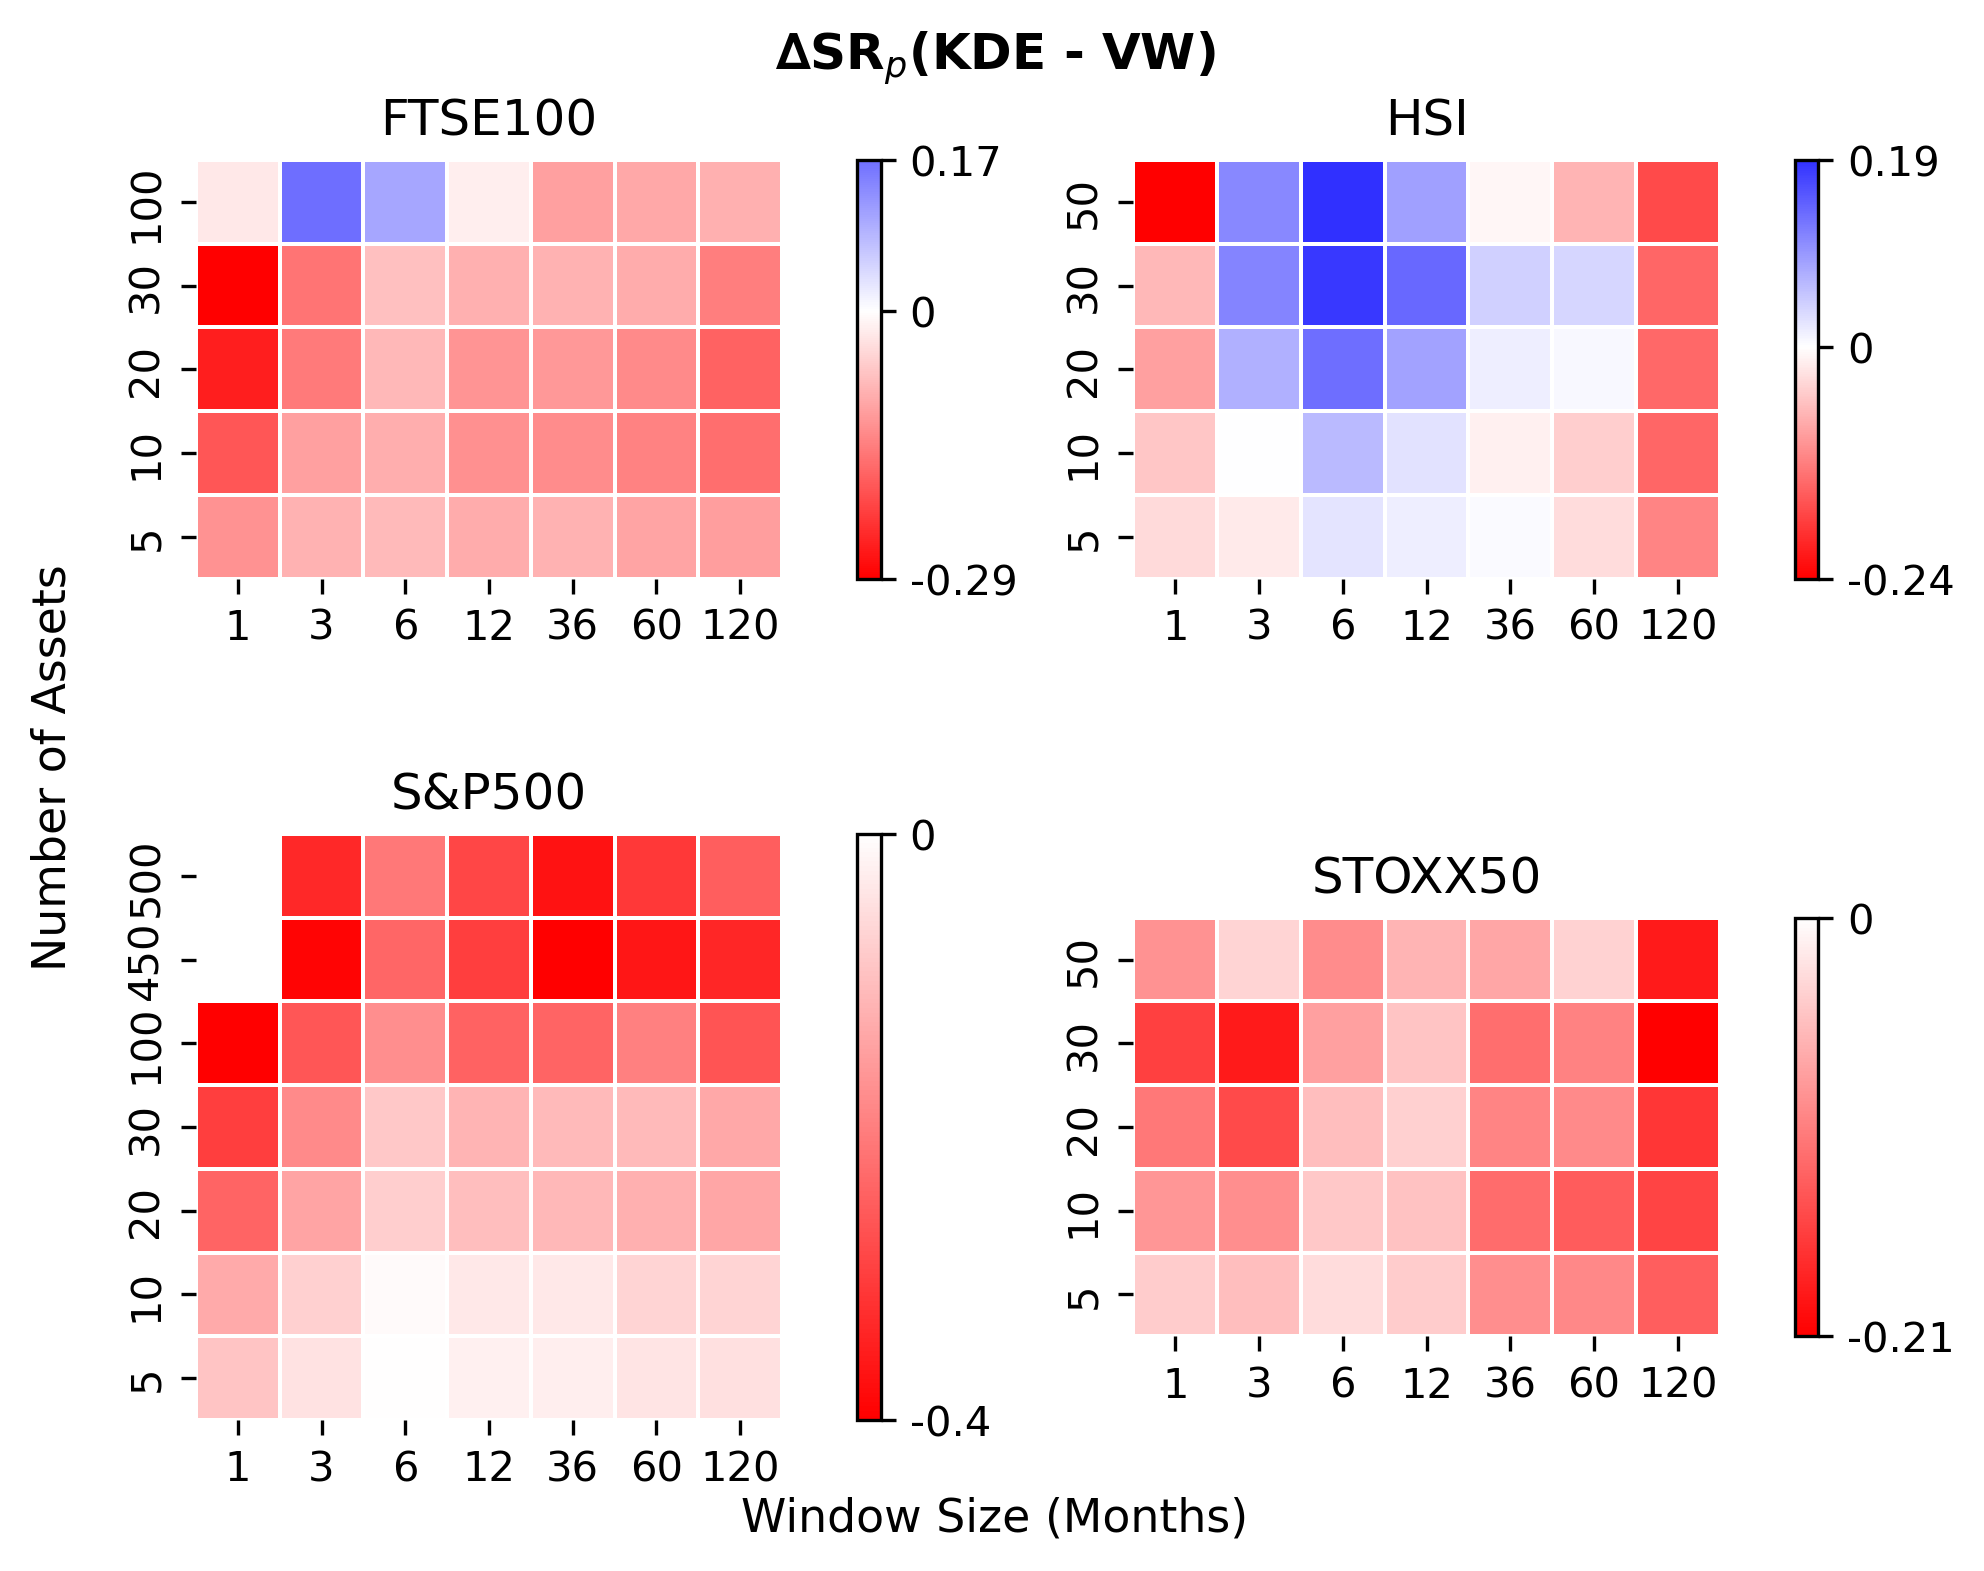
\includegraphics[width=\textwidth]{images/40_14.png}
  \end{minipage}
  \caption[Heatmap 1]{Diverging-color heatmaps of the penalized Sharpe-ratio difference $\Delta SR_p = SR_p(\mathrm{KDE}) - SR_p(\mathrm{VW})$ across model configurations. Each panel shows one index (FTSE100, HSI, S\&P500, STOXX50), with a lookback window (months) on the x-axis and number of assets in the portfolio on the y-axis. Cell color follows a two-slope norm centered at zero. Blue always represents an improvement; red always represents a shortfall. The side color bars indicate the mapping of $\Delta SR_p$ values.}
  \label{fig:combined13}
  \end{center}
  \end{figure}

Compared to the VW portfolio, vanilla KDE outperforms in only 18\% of the grid, with a mean uplift of +9\% in penalized Sharpe Ratio and a mean shortfall of -13\% when it underperforms. Notably, this overperformance comes mainly from the HSI index, clustered around a 6-month data window with approximately 50 assets. A similar comparison performed below with GMM leads us to believe that this is not necessarily a sign of the aptitude of parametric models in that market, but rather a sign of the inaptitude of the VW portfolio.

Comparing against the MAR portfolio raises KDE's win-rate to 59\%, which is especially pronounced for lookback windows of 12 months or less, with an average $SR_{p}$ gain of +13\%. This advantage gradually wanes as the number of assets expands toward full-index universes.

\begin{figure}[H]
  \begin{center}
  \begin{minipage}{1\textwidth}
    \centering
    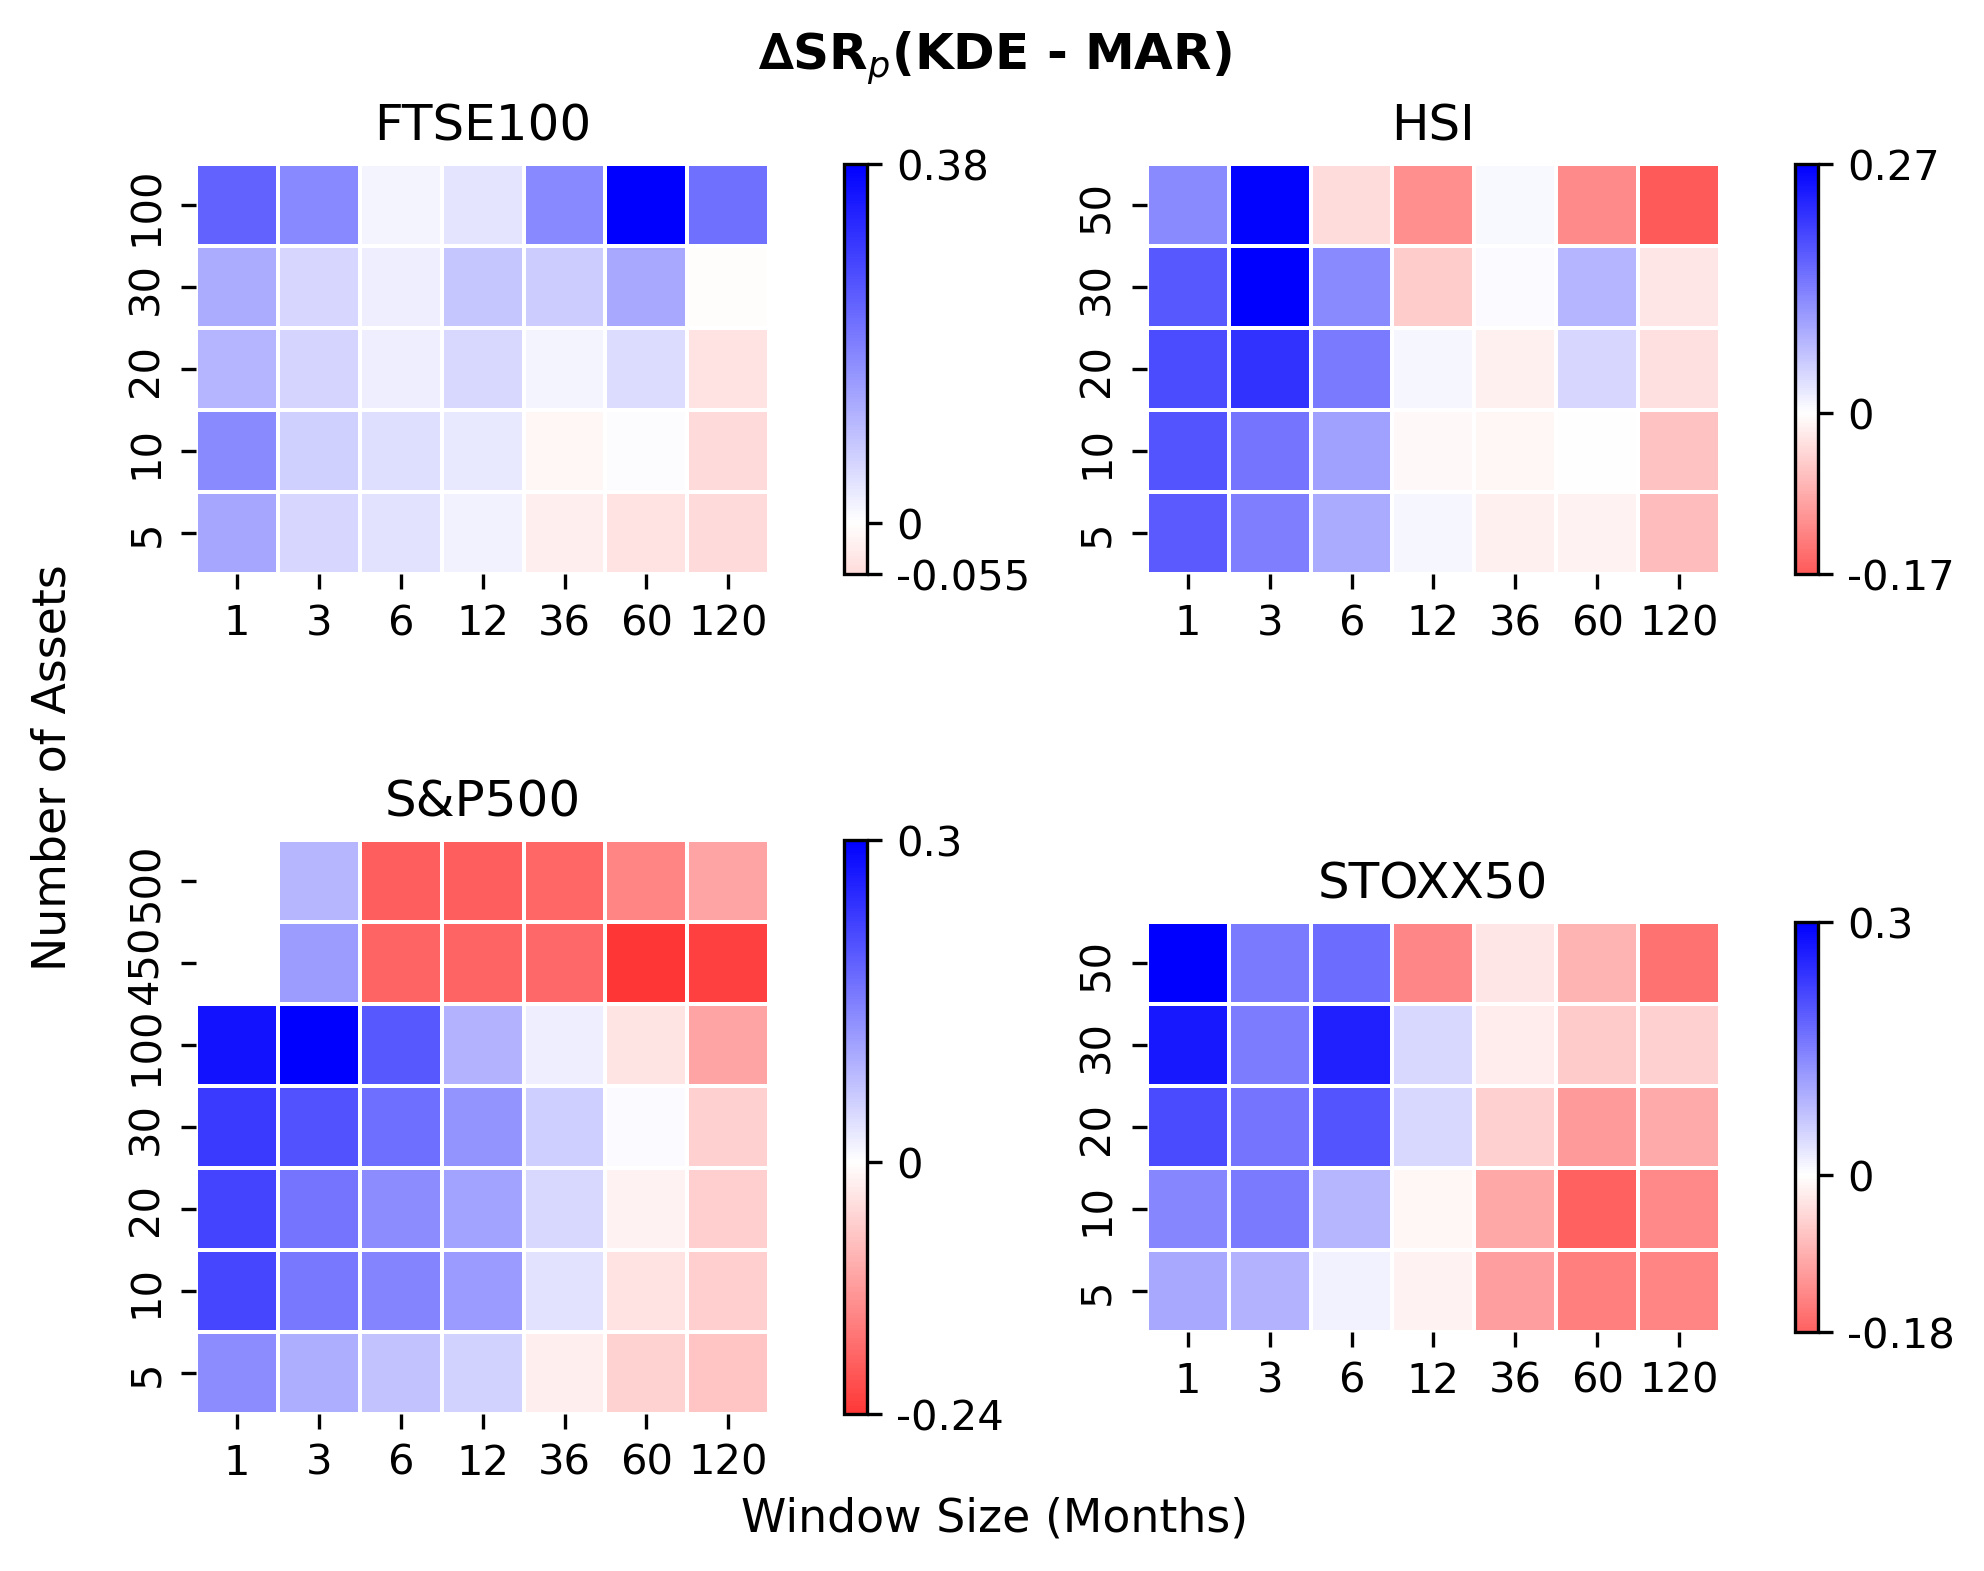
\includegraphics[width=\textwidth]{images/40_15.png}
  \end{minipage}
  \caption[Heatmap 2]{Diverging-color heatmaps of the penalized Sharpe-ratio difference $\Delta SR_p = SR_p(\mathrm{KDE}) - SR_p(\mathrm{MAR})$ across model configurations. Otherwise identical to Figure \ref{fig:combined13}.}
  \label{fig:combined14}
  \end{center}
  \end{figure}

The tangency variant of KDE yields the highest improvements in terms of $SR_{p}$. TAN(KDE) exceeds the classic tangency portfolio in 83\% of configurations, delivering an improvement of +3\%, and a decrease of -2\% on average. This consistency holds across both monthly and annual rebalancing frequencies, window sizes, and numbers of investable assets.

\begin{figure}[H]
  \begin{center}
  \begin{minipage}{1\textwidth}
    \centering
    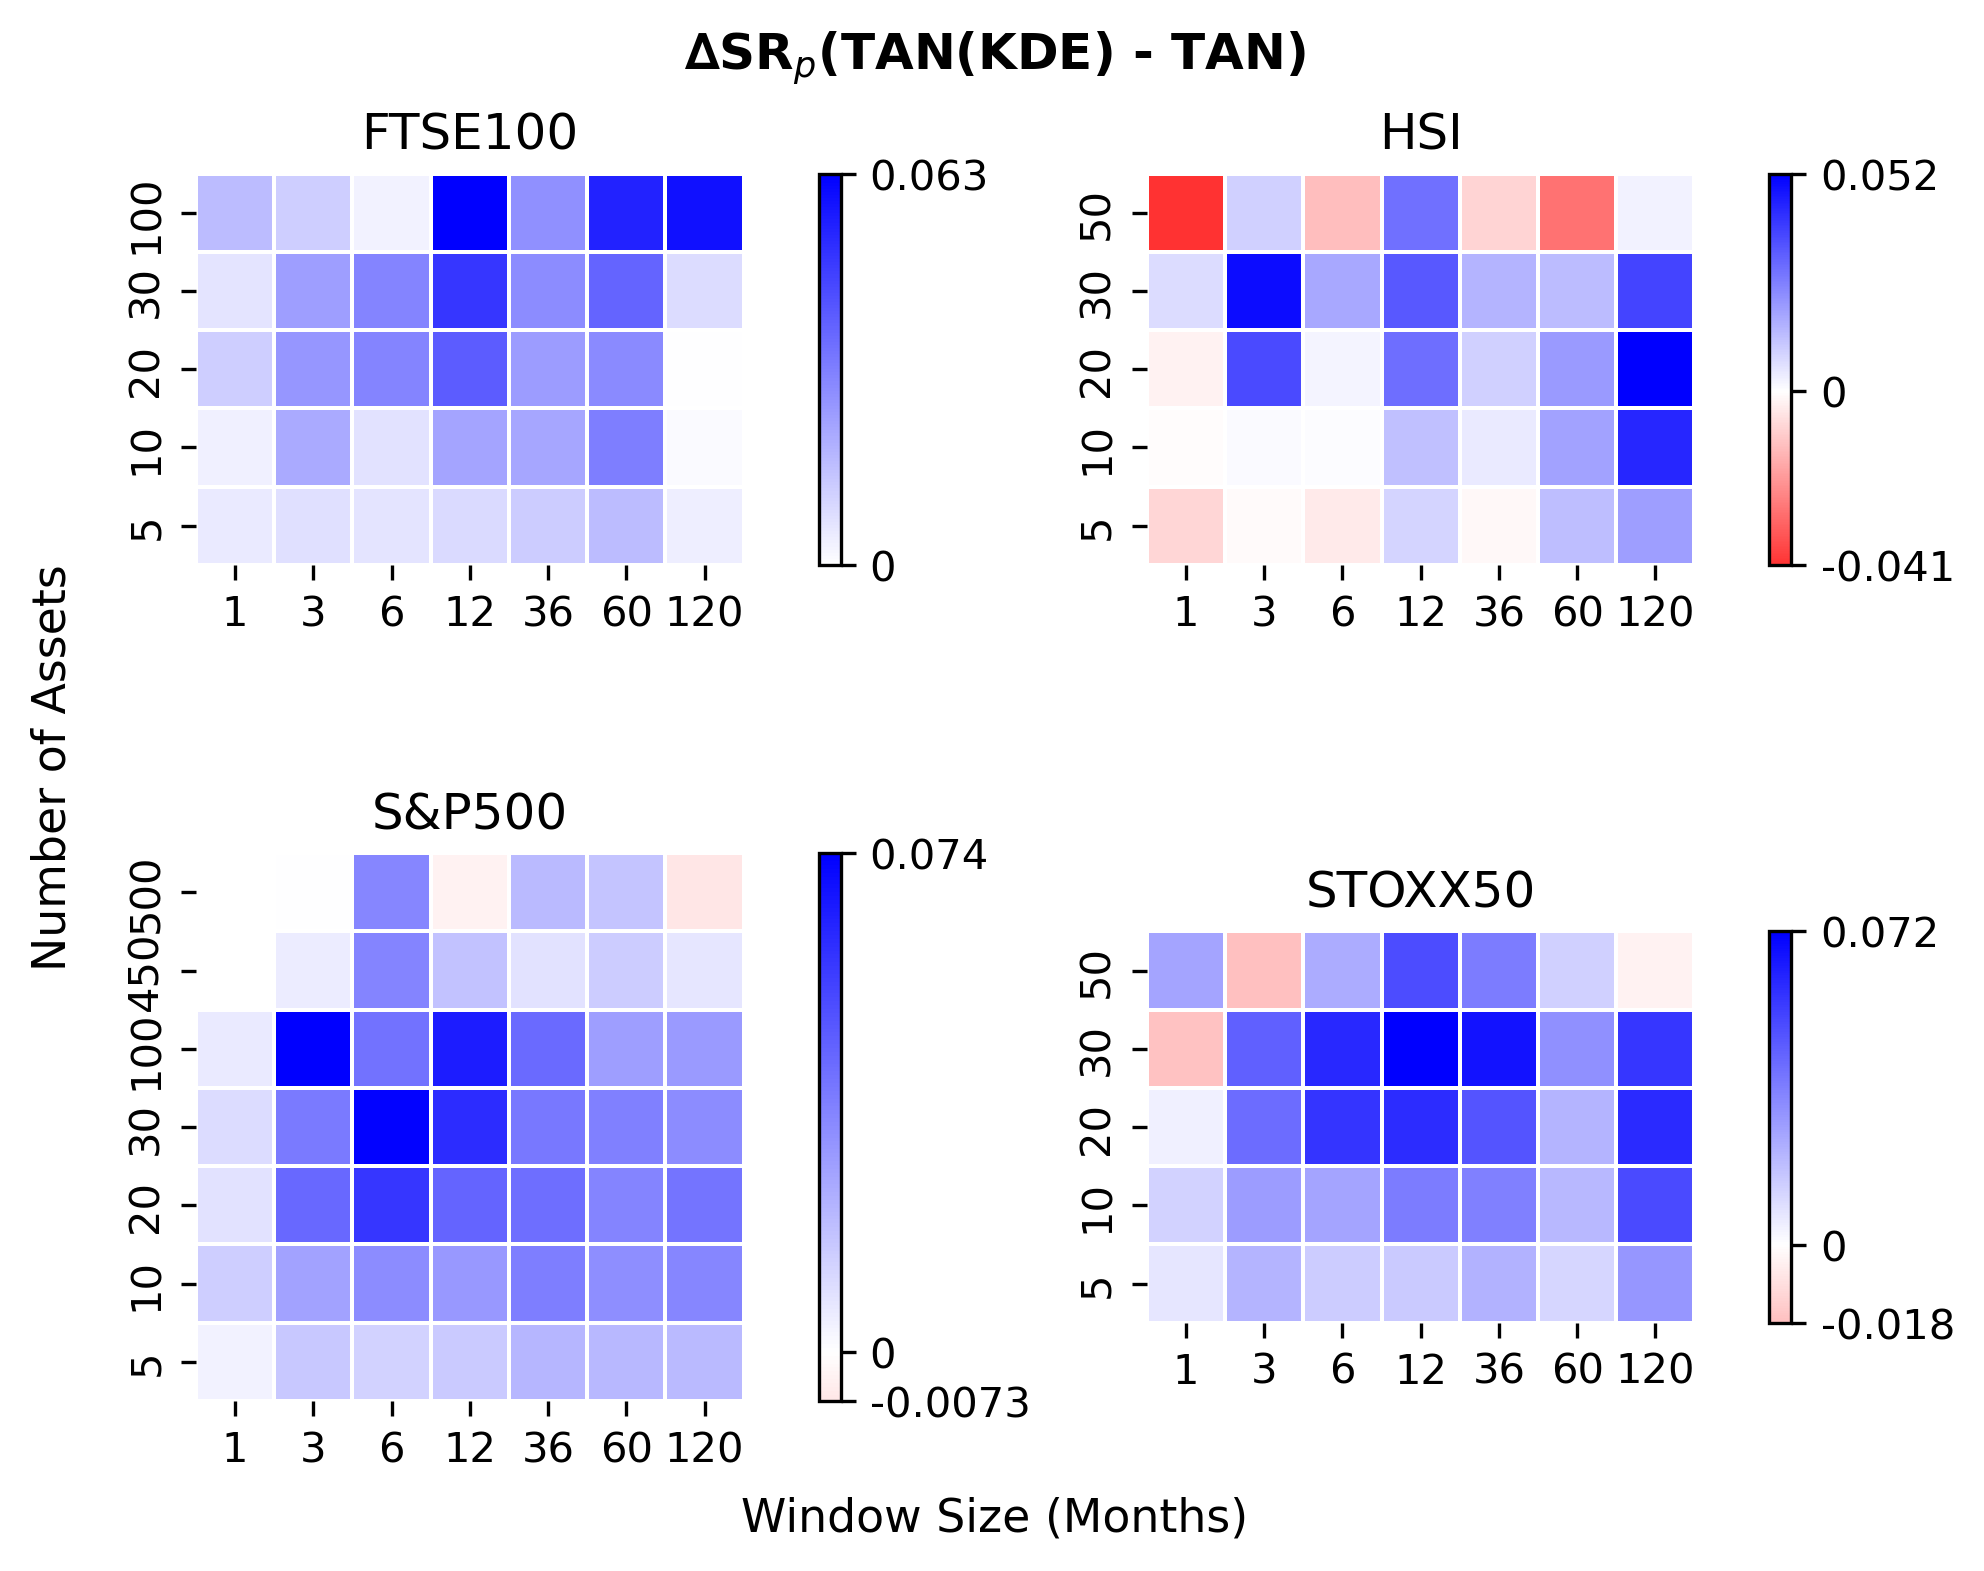
\includegraphics[width=\textwidth]{images/40_16.png}
  \end{minipage}
  \caption[Heatmap 3]{Diverging-color heatmaps of the maximum drawdown difference $\Delta \text{DD} = \text{DD}(\mathrm{KDE}) - \text{DD}(\mathrm{MV})$ across model configurations. A blue cell indicates a decrease in drawdown. Otherwise identical to Figure \ref{fig:combined13}.}
  \label{fig:combined15}
  \end{center}
  \end{figure}

KDE mildly underperforms the MV on maximum drawdown. It reduces $DD$ in 46\% of cases by 3\% points on average, with modest peak improvements at 17\%. TAN(KDE) wins only 25\% of the time but, when successful, can improve drawdown mitigation by 22\% points. Over- and underperformance clusters in certain configuration regions, but this varies by index. Therefore, the choice between KDE-type or MV strategies should be tuned to the market if downside protection is the objective.

\begin{figure}[H]
  \begin{center}
  \begin{minipage}{1\textwidth}
    \centering
    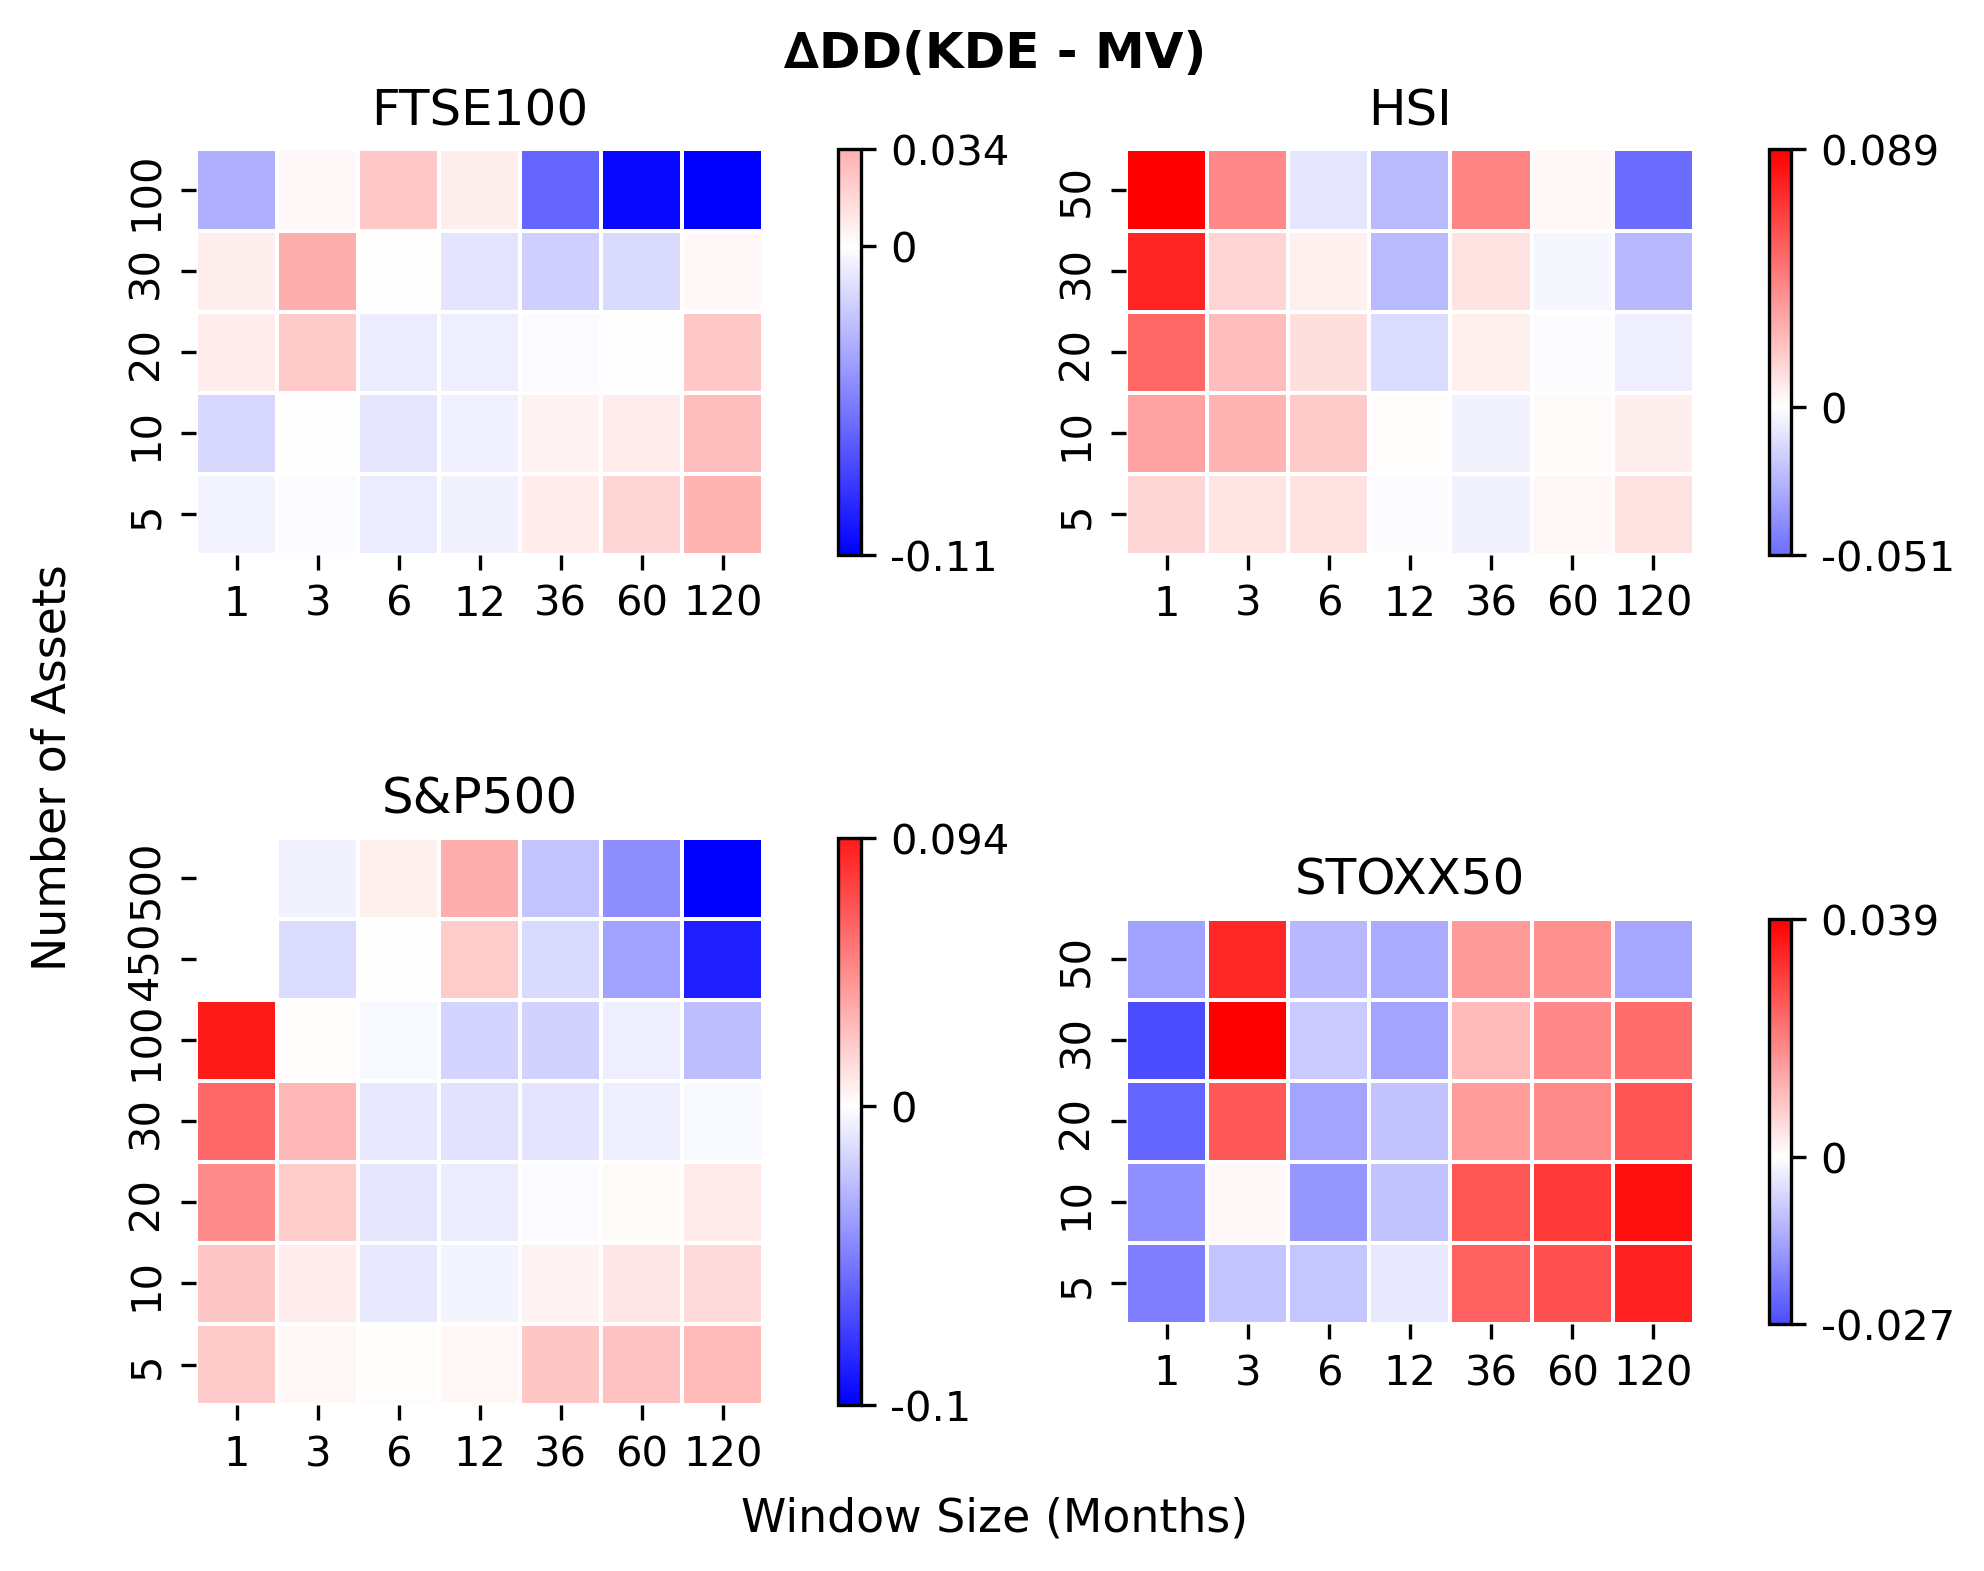
\includegraphics[width=\textwidth]{images/40_17.png}
  \end{minipage}
  \caption[Heatmap 4]{Diverging-color heatmaps of the penalized Sharpe-ratio difference $\Delta SR_p = SR_p(\mathrm{TAN(KDE)}) - SR_p(\mathrm{TAN})$ across model configurations. Otherwise identical to Figure \ref{fig:combined13}.}
  \label{fig:combined16}
  \end{center}
  \end{figure}

Both GMM flavors underperform nearly universally. GMM beats VW by $SR_{p}$ in only 7\% of configurations, and TAN(GMM) in 15\%. Both worsen drawdowns versus MV in over 90\% of configurations. On average, the $DD$ is inflated by 7\% points, while the mean reduction is only 3\% points. The lone "blue" patch appears for TAN(GMM) in the HSI, where, as we noted previously, it is likely that VW itself struggles. We believe that VW's underperformance is the most probable explanation, since the clusters of overperformance for both KDE and GMM are almost exactly in the same configuration region.

\begin{figure}[H]
  \begin{center}
  \begin{minipage}{1\textwidth}
    \centering
    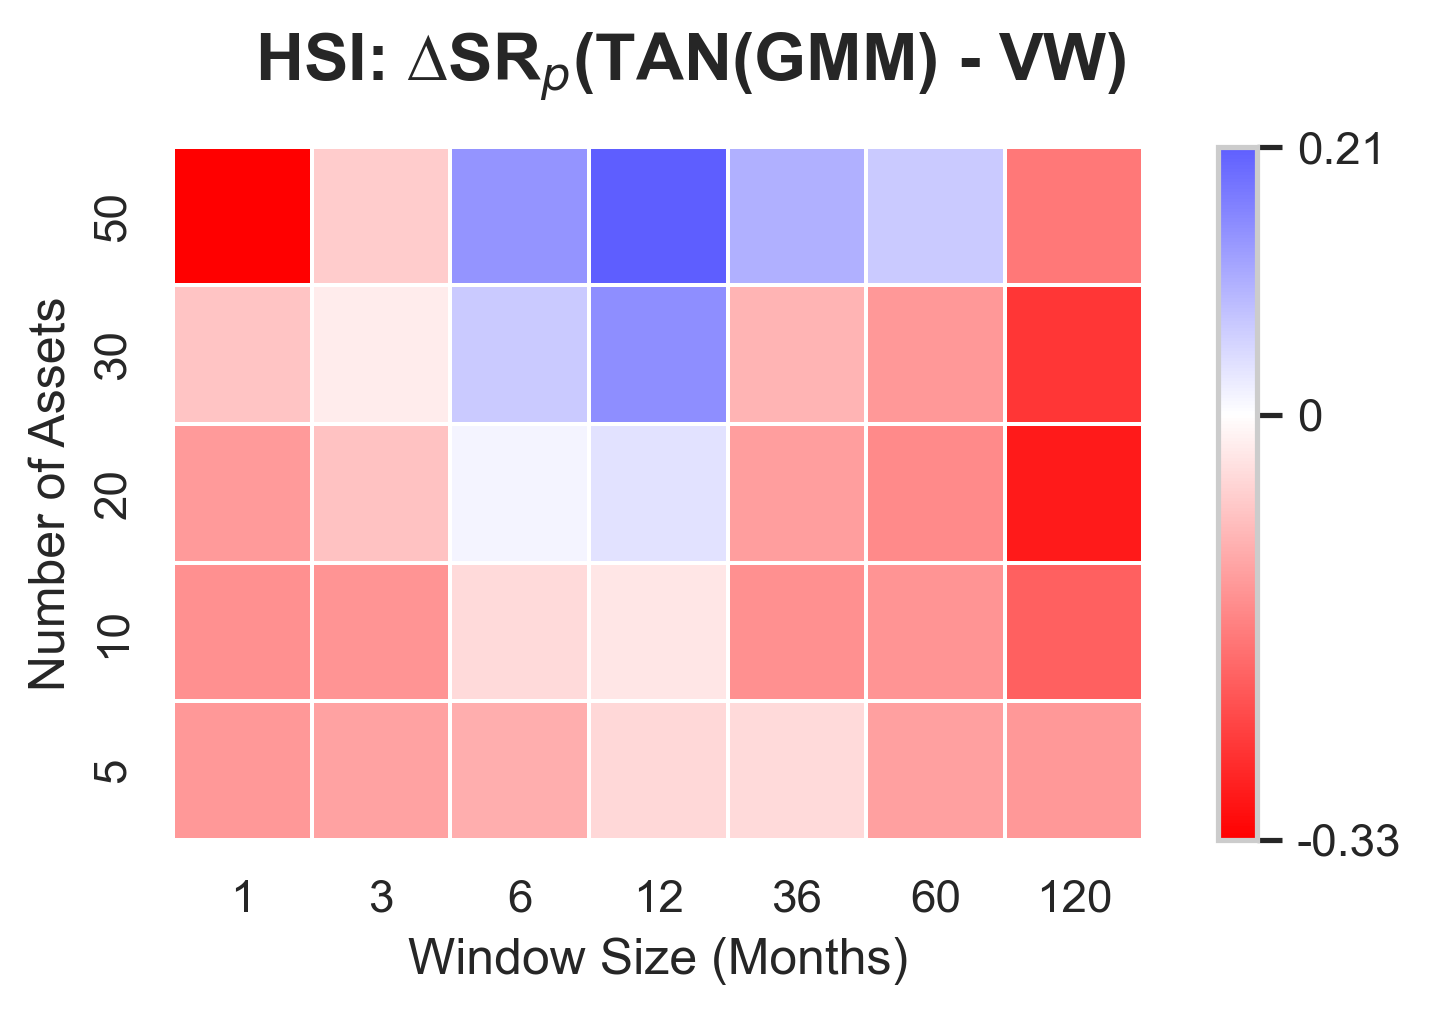
\includegraphics[width=0.5\textwidth]{images/40_18.png}
  \end{minipage}
  \caption[Heatmap 5]{Diverging-color heatmap of the penalized Sharpe-ratio difference $\Delta SR_p = SR_p(\mathrm{TAN(GMM)}) - SR_p(\mathrm{VW})$ across model configurations on the HSI index. Otherwise identical to Figure \ref{fig:combined13}.}
  \label{fig:combined17}
  \end{center}
  \end{figure}

All in all, KDE, especially KDE(TAN), can provide a repeatable enhancement over traditional benchmarks. KDE(TAN) is preferable to TAN across most configurations. KDE is preferable to MAR when the investment universe is moderate ($N \lesssim 100$) and lookback windows are less than a year. Outside this configuration sweet spot, VW or MV remain the safer defaults. By contrast, GMM's high variance and narrow win regions render it unattractive in most scenarios. In the next section, we focus specifically on the KDE and TAN(KDE) portfolios.

\section{CART analysis}
While the heatmaps make it easy to spot the blue regions where the KDE portfolios add value, they do not translate those patches into operational rules. To turn the visual hints into explicit decision criteria, we now fit a set of shallow classification trees. Using the 828 stable configurations that survive our 10\% observation-to-asset filter, we train depth-3 CART models to predict whether a given density-based portfolio beats its benchmark (i.e., whether $\Delta SR_{p}>0$ or $\Delta DD>0$). The input features are data frequency, look-back window (in months), universe size N, and the index. Rebalancing frequency did not improve accuracy and was excluded. The trained tree accuracy ranges from 0.71 to 0.85, suggesting that the splits capture the general structure without overfitting. The results below are grouped by the comparison metric. Because the decision-tree diagrams are visually dense and add little incremental intuition once their verbal rules are stated, we place the full plots in Appendix \ref{app:decisiontrees}.

\newpage
\textbf{Penalized Sharpe Ratio:}
For $\Delta SR_{p}(\text{KDE} - \text{VW})$, KDE outperforms only in two specific regions. In the HSI, it wins when using daily or weekly data and windows between 6 and 12 months. In the STOXX50, the edge appears with monthly data, small universes ($N \le 25$), and 6 to 12 months windows. $\Delta SR_{p}$ is negative elsewhere.

When comparing TAN(KDE) to VW, the advantage holds when $N > 25$ and the lookback is between 6 and 60 months. The performance difference is highly negative in the FTSE100 for ultra-short windows (1-3 months), and negligible in HSI and STOXX when the universe is small.

Against classical TAN, the TAN(KDE) portfolios outperform when using daily or weekly data with $N \le 40$ and windows of 60 to 120 months. Some additional gains persist for $N > 75$ under weekly or monthly data, but they are smaller.

\textbf{Maximum Drawdown:}
For drawdown control, KDE outperforms MV when daily data and long windows (6-120 months) are used. If the data frequency is weekly or monthly, KDE requires a small universe ($N \le 25$) and short windows ($\le 12$ months) to offer any advantage.

TAN(KDE) shows the clearest improvement over MV in larger universes ($N > 75$) with windows of 36 months or more, using daily or weekly data. Monthly frequency removes the advantage unless $N \le 25$.

% \textbf{Conclusion}
\subsection{Practical Summary}
Across the same configuration grid, GMM does not add value. It wins in fewer than 14\% of cases and increases drawdowns in over 90\%. Its trees collapse to trivial structures that predict consistent underperformance. Thus, only KDE-type strategies, applied in the regimes above, offer a repeatable edge over traditional portfolios. Below is a rule of thumb checklist for practitioners wishing to select the appropriate strategy:

\begin{enumerate}
\item High Sharpe Ratio: TAN(KDE), monthly data, 6-60 month window, any index  
\item Control tail-risk in large universes: baseline KDE, daily data, 6-120 month window, $N > 25$ (avoid STOXX50)
\item Short return histories ($\le 12$ months): use KDE over MAR; choose TAN(KDE) if return is the priority over volatility
\item Outside these regimes: default to VW for higher returns, MV for lower risk
\end{enumerate}

\newpage
\section{Limitations \& Path for Future Work}
\label{sec:limitations}
This section provides an overview of the limitations acknowledged in Section \ref{sec:introlimitations}, alongside rationales and suggestions for future research.

The absence of a KDE and GMM minimum-variance benchmark arises from analytical complexities. Specifically, the risk aversion term embedded within the log-sum-exponent structure cannot be factored out easily. This precludes a straightforward analytical derivation of the minimum-variance portfolio, as the usual limit taken to derive it cannot be performed directly. While the most straightforward alternative would be a numerical optimization procedure that iteratively searches through various risk-aversion parameters until the lowest variance is achieved, such an approach lies beyond the scope of this analysis. That is not to say that a closed-form formulation does not exist, but we were unable to derive it in a reasonable time. Hence, the derivation and application of minimum-variance strategies remain avenues for future research.

Similarly, we have not modeled transaction costs or portfolio turnover explicitly due to the practical infeasibility of doing so in the scope of exploring a large configuration space. Storing returns data alone required more than 40 GB of space; storing full weight timeseries for every configuration would have significantly increased the storage requirements further. Future studies may benefit from a targeted analysis of turnover and associated transaction costs.

In the main empirical analysis, we restricted KDE portfolios to strictly positive bandwidths ($H>0$). Ex-ante, this was prudent: a bandwidth of $H=0$ collapses the kernel to a discrete 'spike' density at each observation, which is mathematically consistent but prone to overfitting. Only after completing the out-of-sample evaluation did the visual inspection of portfolio frontiers (Section \ref{sec:frontier}) reveal that KDE's performance primarily arises from its adaptive weighting rather than smoothing effects. Thus, empirically validating the $H=0$ configuration emerges as a natural direction for future research.

Our choice of a 10\% observation-to-asset ratio cutoff for stable configurations was pragmatic, albeit based on ad-hoc considerations. Below that level, the training sample contains, on average, fewer than one year of monthly returns per asset, at which point all Markowitz-type strategies become numerically unstable and the resulting portfolios exhibit large swings in penalised Sharpe across seeds. Raising the threshold further removed only a few additional configurations, yet did not materially change any ranking of strategies, while lowering it to 5\% re-introduced the extreme S\&P500 outcomes that first alerted us to the problem. Thus, 10\% served as the smallest filter that eliminated the problematic cases without discarding a large portion of the configuration grid.

Our empirical analysis has focused on exploring a wide spectrum of portfolio strategies, but future research would benefit from a narrower focus on specific promising configurations. Additionally, the use of intraday data and explicitly examining market-timing strategies may prove to be insightful.

Finally, while KDE addresses the Markowitz assumption of normality, it leaves unchallenged the assumption of distributional stability over time. Significant value may be added by modeling temporal changes in distributions rather than static distributions. An accessible starting point, using only price data, would be integrating return forecasts from ARMA-GARCH models into the KDE framework.
\chapter{Conclusion}
\label{chap:conclusion}
\lhead{Chapter 5. \emph{Conclusion}}
\vspace*{-1\baselineskip}

In this paper, we extend Markowitz's mean-variance framework by embedding skewness directly through mixture density estimators. Applying GMM and KDE to exponential-utility maximization allows us to bypass the need for additional skewness parameters or complex behavioral models. Central to both results is the log-sum-exponent operator, which elevates adverse outcomes in proportion to the risk-aversion parameter $\gamma$. As a result, $\gamma$ now governs both variance and skewness without sacrificing convexity or analytical tractability.

We have shown that replacing the single-Gaussian return assumption with a GMM or KDE density causes a log-sum-exponent weighting to appear naturally inside the exponential-utility objective. That single structural change allows mean-variance optimization to internalize skewness without explicit modeling of extra moments, additional parameters, complex behavioral models, or numerical fragility. The LSE re-weights each historical return in proportion to its disutility, letting the usual risk-aversion parameter $\gamma$ penalize both variance and left-tail outcomes, while keeping the optimization problem convex.

The efficient frontiers of this mechanism lead to three well-defined regimes. When risk aversion is low ($\gamma<\bar{\gamma}$), the optimal solution mimics the standard Markowitz frontier and pursues high expected returns. At the endogenous threshold $\gamma=\bar{\gamma}$, emerges the modified minimum-variance portfolio, which balances the tradeoff between expected returns, variance and tail-risk. Beyond the threshold $\gamma>\bar{\gamma}$, the model willingly accepts higher volatility in order to achieve positive skewness.

Our empirical analysis compares density-weighted approaches across multiple equity indices. Kernel density estimators perform robustly, as their returns remain stable out of sample. Gaussian mixtures show potential on their in-sample frontiers, but fall short when performance dispersion is considered. This lack of performance consistency is exacerbated by the computational cost of the EM algorithm. Kernel density estimation, by contrast, can avoid parameter estimation entirely.

In addition to the suggestions offered in Section \ref{sec:limitations}, future work should test whether the LSE mechanism offers improvements to other return-driven strategies, such as equal-risk-contribution. Even so, our approach embeds skewness seamlessly into Markowitz's mean-variance framework, uniting variance and skewness aversion under a single risk-aversion parameter. By requiring practitioners only to tune $\gamma$, this framework resolves the practical and analytical challenges of non-Gaussian returns and provides a straightforward enhancement to classical portfolio construction.

%----------------------------------------------------------------
% \backmatter
\phantomsection
\addcontentsline{toc}{chapter}{Bibliography}
\bibliographystyle{plainnat}
\bibliography{Bibliography}
\appendix
\chapter[Appendix]{}

\section{Full KDE Portfolio Derivation}
\label{app:kde}
\begin{align*}
  \mathbb{E}[U(R(\mathbf{w}))] &= -\frac{1}{n}\sum_{i=1}^{n}\exp\left(-\gamma\mathbf{w}^{\mathsf{T}}\mathbf{r}_i+\frac{1}{2}\gamma^2\mathbf{w}^{\mathsf{T}}\mathbf{H}\mathbf{w}\right) \\
  &= -\frac{1}{n}\exp\left(\frac{1}{2}\gamma^2\mathbf{w}^{\mathsf{T}}\mathbf{H}\mathbf{w}\right)\sum_{i=1}^{n}\exp\left(-\gamma\mathbf{w}^{\mathsf{T}}\mathbf{r}_i\right) \\
  \intertext{Maximizing the expected utility:}
  \arg\max_\mathbf{w}{\mathbb{E}[U(R(\mathbf{w}))]} &= \arg\max_\mathbf{w}{-\frac{1}{n}\exp\left(\frac{1}{2}\gamma^2\mathbf{w}^{\mathsf{T}}\mathbf{H}\mathbf{w}\right)\sum_{i=1}^{n}\exp\left(-\gamma\mathbf{w}^{\mathsf{T}}\mathbf{r}_i\right)} \\
  &= \arg\min_\mathbf{w}{{\frac{1}{n}\exp\left(\frac{1}{2}\gamma^2\mathbf{w}^{\mathsf{T}}\mathbf{H}\mathbf{w}\right)\sum_{i=1}^{n}\exp\left(-\gamma\mathbf{w}^{\mathsf{T}}\mathbf{r}_i\right)}} \\
  &= \arg\min_\mathbf{w}\log{{{\frac{1}{n}\exp\left(\frac{1}{2}\gamma^2\mathbf{w}^{\mathsf{T}}\mathbf{H}\mathbf{w}\right)\sum_{i=1}^{n}\exp\left(-\gamma\mathbf{w}^{\mathsf{T}}\mathbf{r}_i\right)}}} \\
  &= \arg\min_\mathbf{w}{\frac{1}{2}\gamma^2\mathbf{w}^{\mathsf{T}}\mathbf{H}\mathbf{w}+\log{\left[\sum_{i=1}^{n}\exp\left(-\gamma\mathbf{w}^{\mathsf{T}}\mathbf{r}_i\right)\right]}}-\log n \\
  &= \arg\min_\mathbf{w}\frac{1}{2}\gamma^2\mathbf{w}^{\mathsf{T}}\mathbf{H}\mathbf{w}+LSE(-\gamma\mathbf{w}^{\mathsf{T}}\mathbf{r}_i)-\log n
  \end{align*}

Setting up Lagrangian and imposing the fully invested constraint:
$$\mathcal{L}=\frac{1}{2}\gamma^2\mathbf{w}^{\mathsf{T}}\mathbf{H}\mathbf{w}+LSE(-\gamma\mathbf{w}^{\mathsf{T}}\mathbf{r}_i)+\lambda(\mathbf{w^{\mathsf{T}}1}-1)$$

Define:
$$f_i(\mathbf{w})=-\gamma\mathbf{w}^{\mathsf{T}}\mathbf{r}_i$$
$$\Longrightarrow \mathcal{L}=\frac{1}{2}\gamma^2\mathbf{w}^{\mathsf{T}}\mathbf{H}\mathbf{w}+LSE(-\gamma\mathbf{w}^{\mathsf{T}}\mathbf{r}_i)+\lambda(\mathbf{w^{\mathsf{T}}1}-1)$$
$$\frac{\partial\mathcal{L}}{\partial\mathbf{w}}=\frac{\partial}{\partial\mathbf{w}}LSE_i(f_i(\mathbf{w}))+\gamma^2\mathbf{H}\mathbf{w}+\lambda\mathbf{1}$$
\begin{align*}
\frac{\partial}{\partial\mathbf{w}}LSE_i(f_i(\mathbf{w}))&=\frac{\partial}{\partial\mathbf{w}}\log{\left[{\sum_{i=1}^{n}\exp f_i(\mathbf{w})}\right]} \\
&=\frac{1}{\sum_{i=1}^{n}\exp f_i(\mathbf{w})}\cdot\frac{\partial}{\partial\mathbf{w}}\left[{\sum_{i=1}^{n}\exp f_i(\mathbf{w})}\right] \\
&=\frac{1}{\sum_{i=1}^{n}\exp f_i(\mathbf{w})}\left[{\sum_{i=1}^{n}\exp f_i(\mathbf{w})}\cdot\frac{\partial}{\partial\mathbf{w}}f_i(\mathbf{w})\right] \\
&=\frac{1}{\sum_{i=1}^{n}\exp f_i(\mathbf{w})}\left[{\sum_{i=1}^{n}\exp f_i(\mathbf{w})}\cdot\frac{\partial}{\partial\mathbf{w}}f_i(\mathbf{w})\right] \\
&\frac{\partial}{\partial\mathbf{w}}f_i(\mathbf{w})=-\gamma\mathbf{r}_i \\
\Longrightarrow \frac{\partial}{\partial\mathbf{w}}LSE_i(f_i(\mathbf{w}))&=\frac{{\sum_{i=1}^{n}\exp f_i(\mathbf{w})}\cdot(-\gamma\mathbf{r}_i)}{\sum_{i=1}^{n}\exp f_i(\mathbf{w})}
\end{align*}

Recognizing the softmax function
\begin{align*}
  &\quad\frac{{\exp f_i(\mathbf{w})}}{\sum_{i=1}^{n}\exp f_i(\mathbf{w})}\equiv p_i \\
  \frac{\partial\mathcal{L}}{\partial\mathbf{w}}:\quad&\sum_{i=1}^{n}p_i(-\gamma\mathbf{r}_i)+\gamma^2\mathbf{H}\mathbf{w}+\lambda\mathbf{1}=0 \\
  =&\gamma^2\mathbf{H}\mathbf{w}-\gamma\sum_{i=1}^{n}p_i\mathbf{r}_i+\lambda\mathbf{1}=0
\end{align*}

Denoting for brevity
$$c\equiv\sum_{i=1}^{n}p_i\mathbf{r}_i$$
$$\Longrightarrow\gamma^{2}\mathbf{H}\mathbf{w}-\gamma c+\lambda\mathbf{1}=0$$
$$\mathbf{w}=\mathbf{H}^{-1}\left(\frac{\gamma}{\gamma^{2}}c-\frac{\lambda}{\gamma^{2}}\mathbf{1}\right)$$
$$1=\frac{\gamma}{\gamma^{2}}\mathbf{1}^{\mathsf{T}}\mathbf{H}^{-1}c-\frac{\lambda}{\gamma^{2}}\mathbf{1}^{\mathsf{T}}\mathbf{H}^{-1}\mathbf{1}$$
$$-\frac{\lambda}{\gamma^{2}}=\frac{1-\frac{1}{\gamma}\mathbf{1}^{\mathsf{T}}\mathbf{H}^{-1}c}{\mathbf1^T \mathbf{H}^{-1}\mathbf1}$$
$$\Longrightarrow\mathbf{w}^*=\frac{1}{\gamma}\mathbf{H}^{-1}c+\left(\frac{1-\frac{1}{\gamma}\mathbf{1}^{\mathsf{T}}\mathbf{H}^{-1}c}{\mathbf1^T \mathbf{H}^{-1}\mathbf1}\right)\mathbf{H}^{-1}\mathbf{1}$$
$$\boxed{\mathbf{w}^*=\frac{1}{\gamma}\mathbf{H}^{-1}c+\left(\frac{1}{\mathbf1^T H^{-1}\mathbf1}-\frac{1}{\gamma}\frac{\mathbf{1}^{\mathsf{T}}\mathbf{H}^{-1}c}{\mathbf1^T H^{-1}\mathbf1}\right)\mathbf{H}^{-1}\mathbf{1}}$$
with
$$c\equiv \sum_{i=1}^{n} \frac{\exp f_i(\mathbf{w})}{\sum_{j=1}^{n} \exp f_j(\mathbf{w})} \mathbf{r}_i$$

\section{LSE Jacobian \& Hessian}
\label{app:lse}
Suppose we have a vector valued, twice-differentiable function: 
$$f(\mathbf{w})=(f_1(\mathbf{w}), f_2(\mathbf{w}),...,f_k(\mathbf{w}))^{\mathsf{T}}$$

It's Jacobian matrix is:
$$\mathbf{J}_f=\begin{bmatrix} \frac{\partial f_1}{\partial w_{1}}, \frac{\partial f_1}{\partial w_{2}}, \dots,\frac{\partial f_1}{\partial w_{n}} \\ \frac{\partial f_2}{\partial w_{1}}, \frac{\partial f_2}{\partial w_{2}}, \dots,\frac{\partial f_2}{\partial w_{n}} \\ \vdots \\ \frac{\partial f_k}{\partial w_{1}}, \frac{\partial f_k}{\partial w_{2}}, \dots,\frac{\partial f_k}{\partial w_{n}}\end{bmatrix} = \begin{bmatrix} \nabla f_1(\mathbf{w})^{\mathsf{T}}\\ \nabla f_2(\mathbf{w})^{\mathsf{T}} \\ \vdots \\ \nabla f_k(\mathbf{w})^{\mathsf{T}}\end{bmatrix}$$

And the log-sum-exponent function that takes $f_i(\mathbf{w})$ as an argument:
$$LSE_i(f_i(\mathbf{w}))=\log{\left[\sum_{i=1}^{k}\exp(f_i(\mathbf{w}))\right]}$$

---
Gradient
$$l(\mathbf{w})=\log{\left[\sum_{i=1}^{k}\exp(f_i(\mathbf{w}))\right]}\equiv \log(s), \qquad s=\sum_{i=1}^{k}\exp(f_i(\mathbf{w}))$$

$$\frac{\partial l}{\partial w_j}=\frac{1}{s}\cdot\frac{\partial}{\partial w_i}s$$

$$\frac{\partial}{\partial w_j}s=\sum_{i=1}^{k}\frac{\partial}{\partial w_j}\exp(f_i(\mathbf{w}))=\sum_{i=1}^{k}\exp(f_i(\mathbf{w}))\cdot\frac{\partial}{\partial w_j}f_i(\mathbf{w})$$

$$\Longrightarrow\frac{\partial l}{\partial w_j}=\frac{1}{s}\cdot\sum_{i=1}^{k}\exp(f_i(\mathbf{w}))\cdot\frac{\partial}{\partial w_j}f_i(\mathbf{w})$$

$$=\sum_{i=1}^{k}p_i\cdot\frac{\partial}{\partial w_j}f_i(\mathbf{w})\qquad\text{where}\qquad p_i=\frac{\exp( f_i(\mathbf{w}))}{s}=\frac{{\exp( f_i(\mathbf{w}))}}{\sum_{i=1}^{k}\exp (f_i(\mathbf{w}))}$$

The gradient of log-sum-exponent function with respect to the input vector  $\mathbf{w}$ is the softmax-weighted average of gradients of functions $f_i(\mathbf{w})$.

---
Hessian

$$\Longrightarrow\frac{\partial^2 l}{\partial w_j\partial w_k}=\left(\frac{\partial}{\partial w_k}\frac{1}{s}\right)\cdot\frac{\partial}{\partial w_j}s+\frac{1}{s}\cdot\left(\frac{\partial^2}{\partial w_j\partial w_k}s\right)$$

$$\rightarrow\frac{\partial}{\partial w_j}\frac{1}{s}=-\frac{1}{s^2}\cdot\frac{\partial}{\partial w_j}s=-\frac{1}{s^2}\cdot\sum_{i=1}^{k}\exp(f_i(\mathbf{w}))\cdot\frac{\partial}{\partial w_j}f_i(\mathbf{w})$$

$$\rightarrow\frac{\partial^2}{\partial w_j\partial w_k}s=\frac{\partial}{\partial w_k}\sum_{i=1}^{k}\exp(f_i(\mathbf{w}))\cdot\frac{\partial}{\partial w_j}f_i(\mathbf{w})$$

$$=\sum_{i=1}^{k}\left[\exp(f_i(\mathbf{w}))\cdot\left(\frac{\partial^2}{\partial w_j\partial w_k}f_i(\mathbf{w})\right)+\exp(f_i(\mathbf{w}))\cdot\left(\frac{\partial}{\partial w_k}f_i(\mathbf{w})\right)\left(\frac{\partial}{\partial w_j}f_i(\mathbf{w})\right)\right]$$

$$=\sum_{i=1}^{k}\exp(f_i(\mathbf{w}))\left[\left(\frac{\partial^2}{\partial w_j\partial w_k}f_i(\mathbf{w})\right)+\left(\frac{\partial}{\partial w_k}f_i(\mathbf{w})\right)\left(\frac{\partial}{\partial w_j}f_i(\mathbf{w})\right)\right]$$

Which means that the Hessian is:

$$\Longrightarrow\frac{\partial^2 l}{\partial w_j\partial w_k}=\frac{1}{s}\sum_{i=1}^{k}\exp(f_i(\mathbf{w}))\left[\left(\frac{\partial^2}{\partial w_j\partial w_k}f_i(\mathbf{w})\right)+\left(\frac{\partial}{\partial w_k}f_i(\mathbf{w})\right)\left(\frac{\partial}{\partial w_j}f_i(\mathbf{w})\right)\right]-$$

$$\qquad\qquad\qquad-\frac{1}{s^2}\cdot\left(\sum_{i=1}^{k}\exp(f_i(\mathbf{w}))\cdot\frac{\partial}{\partial w_j}f_i(\mathbf{w})\right)\left(\sum_{i=1}^{k}\exp(f_i(\mathbf{w}))\cdot\frac{\partial}{\partial w_k}f_i(\mathbf{w})\right)$$

$$=\sum_{i=1}^{k}p_i\cdot\left[\mathbf{H}_{f_i}+\mathbf{J}_{f_i}^{}\,\mathbf{J}_{f_i}^{\mathsf{T}}\right]-\left(\sum_{i=1}^{k}p_i\mathbf{J}_{f_i}\right)\left(\sum_{j=1}^{k}p_j\mathbf{J}_{f_i}\right)^{\mathsf{T}}$$

Where $\mathbf{J}_{f_i}$ and $\mathbf{H}_{f_i}$ are the Jacobian and Hessian matrix of function $f_i(\mathbf{w})$ respectively.

$$\sum_{i=1}^{k}p_i\cdot\left[\mathbf{J}_{f_i}^{}\,\mathbf{J}_{f_i}^{\mathsf{T}}\right]-\left(\sum_{i=1}^{k}p_i\mathbf{J}_{f_i}\right)\left(\sum_{j=1}^{k}p_j\mathbf{J}_{f_i}\right)^{\mathsf{T}}$$

\newpage
\section{Average Performance Per Index}
\label{app:avgperf}

\begin{table}[H]
  \centering
  \makebox[\textwidth][c]{\begin{tabular}{ll*{7}{S[table-format=1.4]}}
  \toprule
  Index & Strategy & {$\mu$} & {$\sigma$} & {SR} & {CR} & {VaR} & {DD} & {\textbar DD\textbar} \\
  \midrule
  \multirow{8}{*}{\textbf{FTSE100}} & VW & 0.0804 & {\bfseries 0.1584} & {\bfseries 0.3892} & 0.9427 & 0.2278 & 0.3301 & {\bfseries 2.5994} \\
   & KDE & 0.0760 & 0.1638 & 0.3511 & 0.9171 & 0.2342 & {\bfseries 0.3297} & 3.4286 \\
   & TAN(KDE) & 0.4548 & 0.1787 & 0.3399 & 0.8957 & 0.2558 & 0.3508 & 3.5877 \\
   & MV & 0.0733 & 0.1596 & 0.3390 & 0.8599 & {\bfseries 0.2257} & 0.3342 & 3.4339 \\
   & TAN & 0.4531 & 0.1841 & 0.3235 & 0.8745 & 0.2642 & 0.3620 & 3.8371 \\
   & MAR & 0.4681 & 0.2028 & 0.3223 & {\bfseries 0.9785} & 0.2916 & 0.3951 & 4.1021 \\
   & GMM & 0.4395 & 0.2069 & 0.2915 & 0.8477 & 0.2858 & 0.4024 & 4.3971 \\
   & TAN(GMM) & {\bfseries 1.0399} & 0.2111 & 0.2863 & 0.7454 & 0.2990 & 0.4156 & 4.6076 \\
  \midrule
  \multirow{8}{*}{\textbf{HSI}} & MV & 0.0581 & {\bfseries 0.1582} & {\bfseries 0.2419} & {\bfseries 0.6123} & {\bfseries 0.2454} & {\bfseries 0.3957} & 5.3408 \\
   & KDE & 0.0543 & 0.1645 & 0.2060 & 0.5393 & 0.2571 & 0.4025 & 5.5658 \\
   & TAN(KDE) & {\bfseries 0.0617} & 0.2119 & 0.1917 & 0.5613 & 0.3286 & 0.4952 & {\bfseries 4.8538} \\
   & TAN & 0.0617 & 0.2160 & 0.1865 & 0.5619 & 0.3335 & 0.5077 & 4.8667 \\
   & VW & 0.0588 & 0.1967 & 0.1849 & 0.4943 & 0.3055 & 0.4381 & 5.3854 \\
   & MAR & 0.0579 & 0.2122 & 0.1778 & 0.5165 & 0.3296 & 0.5004 & 5.6071 \\
   & TAN(GMM) & 0.0612 & 0.2392 & 0.1689 & 0.5181 & 0.3629 & 0.5420 & 5.1723 \\
   & GMM & 0.0489 & 0.1918 & 0.1528 & 0.4538 & 0.2956 & 0.4768 & 5.7499 \\
  \midrule
  \multirow{8}{*}{\textbf{S\&P500}} & VW & {\bfseries 0.1387} & 0.1834 & {\bfseries 0.6688} & {\bfseries 2.3173} & 0.2705 & {\bfseries 0.3224} & {\bfseries 1.9773} \\
   & TAN(KDE) & 0.1241 & 0.1889 & 0.5746 & 1.9004 & 0.2765 & 0.3309 & 2.3981 \\
   & TAN & 0.1240 & 0.1945 & 0.5560 & 1.9036 & 0.2842 & 0.3381 & 2.5066 \\
   & KDE & 0.1097 & 0.1773 & 0.5275 & 1.5688 & 0.2537 & 0.3258 & 2.3895 \\
   & MAR & 0.1302 & 0.2220 & 0.5204 & 2.0468 & 0.3242 & 0.3944 & 3.0149 \\
   & MV & 0.1056 & {\bfseries 0.1721} & 0.5158 & 1.4779 & {\bfseries 0.2450} & 0.3265 & 2.3629 \\
   & TAN(GMM) & 0.1168 & 0.2212 & 0.4619 & 1.6950 & 0.3207 & 0.3869 & 3.1961 \\
   & GMM & 0.1052 & 0.2114 & 0.4241 & 1.4505 & 0.3044 & 0.3825 & 3.3585 \\
  \midrule
  \multirow{8}{*}{\textbf{STOXX50}} & VW & 0.1054 & 0.1869 & {\bfseries 0.4530} & 1.3453 & 0.2709 & {\bfseries 0.3296} & {\bfseries 2.2780} \\
   & TAN(KDE) & {\bfseries 0.1084} & 0.1977 & 0.4378 & {\bfseries 1.4304} & 0.2893 & 0.3529 & 3.1432 \\
   & MV & 0.0982 & {\bfseries 0.1764} & 0.4364 & 1.2819 & {\bfseries 0.2529} & 0.3371 & 3.0063 \\
   & TAN & 0.1078 & 0.2052 & 0.4167 & 1.4041 & 0.3015 & 0.3700 & 3.4417 \\
   & KDE & 0.0957 & 0.1838 & 0.4042 & 1.2066 & 0.2667 & 0.3432 & 3.0379 \\
   & MAR & 0.1037 & 0.2103 & 0.3969 & 1.3183 & 0.3087 & 0.3841 & 3.5627 \\
   & TAN(GMM) & 0.1029 & 0.2265 & 0.3601 & 1.2625 & 0.3299 & 0.4100 & 4.0501 \\
   & GMM & 0.0964 & 0.2117 & 0.3531 & 1.1814 & 0.3067 & 0.3943 & 3.8522 \\
  \bottomrule
\end{tabular}
}
  \caption[Per index performance]{Average annualized performance (Jan 2015-Mar 2025) of all portfolio configurations, aggregated by index. The table is sorted within each index block by Sharpe ratio (SR).}
  \label{tab:app:avgperf:combined}
\end{table}


\newpage
\section{Computational Considerations}
\label{app:compute}
The implementation of GMM and KDE portfolio optimization presents several computational challenges. This section outlines our experiences and recommendations for efficient implementation.

\subsection{Optimization Frameworks}
The EM estimation in GMM represents the most computationally intensive step in our implementation. Its complexity grows substantially with both the number of clusters $K$ and the dimensions of the sample window. Despite considerable effort to accelerate this process, we achieved only minimal improvements. This computational burden makes the practical application of optimal $K$ selection discussed in Section \ref{sec:gmmselect} prohibitively expensive for strategies requiring frequent rebalancing.

For portfolio optimization in Python, we initially employed \textit{cvxpy}, which generally serves as an excellent default choice for convex problems. However, while both KDE and GMM formulations are convex, their performance with \textit{cvxpy} deteriorates with large windows. This occurs because \textit{cvxpy} must recompile the problem into a form compatible with its optimization algorithm each time we slide the window of return observations. The resulting compile time grows with both the sample length and the square of the portfolio dimension.

As an alternative, we recommend \textit{cyipopt}, a highly optimized interior-point solver. Unlike \textit{cvxpy}, \textit{cyipopt} requires only that the user provide analytic expressions for the objective's gradient and Hessian once, bypassing all symbolic translation. For KDE optimization, this approach delivered dramatically faster and more optimal solutions.

\subsection{Improving \textit{scipy} Performance}
As a general-purpose solver, \textit{scipy} would not typically be expected to outperform specialized optimization libraries. However, our experience shows that it matches the optimality of \textit{cvxpy} while executing significantly faster for smaller problems (approximately 20-30 assets maximum). It also offers superior stability, making it valuable as a fallback solver when \textit{cvxpy} or \textit{cyipopt} fails, which occasionally occurs even if the problems should be valid in principle.

We found that \textit{scipy}'s performance can be substantially improved through several techniques:

\begin{enumerate}
\item Use solvers that accept user-defined Jacobian functions, such as SLSQP, and provide these functions explicitly. This eliminates the need for \textit{scipy} to approximate function gradients via finite differences.

\item When providing the Jacobian function, set \textit{jac=True} rather than passing the function as a separate argument. This approach requires the objective function to return both the objective value and its gradient as outputs (i.e., \textit{return objective\_value, objective\_gradient}), avoiding redundant computation of matrix multiplications and significantly improving performance.

\item Precompile objective and Jacobian functions. This can be accomplished through simple approaches like adding \textit{numba} decorators to functions, or more involved techniques such as implementing functions in C. In our work, custom C functions delivered order-of-magnitude speed improvements for certain portfolio estimations.
\end{enumerate}

\subsection{General Performance Considerations}
Parallel processing represents perhaps the most significant performance uplift available. While detailed implementation discussion lies beyond our scope, it suffices to say that runtime decreases approximately linearly with the number of allocated workers. In our empirical backtest performed on a MacBook M1 Pro (8-core) with 16GB RAM, parallelization resulted in nearly an 8-fold speed improvement.

Finally, we emphasize the importance of using a platform-aware environment manager like \textit{conda}. Unlike \textit{pip}, \textit{conda} automatically installs pre-built library binaries optimized for specific CPU architectures. This results in significant performance gains for core numerical libraries with no additional implementation effort. In our experience, using \textit{conda} instead of \textit{pip} yielded performance improvements of approximately 20-30\%.

\section{Decision Trees}
\label{app:decisiontrees}

\begin{table}[H]
  \centering
  \
\paragraph{CART: $\Delta$SR$_p$(KDE - VW)}

\begin{flushleft}
\ttfamily %
index ≠ HSI \\
\quad window (1 to 36) \\
\quad \quad window (1) \\
\quad \quad \quad \quad → weights: [100\% ≤ 0, 0\% > 0] ⇒ predict Δ ≤ 0 \\
\quad \quad window (3 to 120) \\
\quad \quad \quad index ≠ STOXX50 \\
\quad \quad \quad \quad → weights: [70\% ≤ 0, 30\% > 0] ⇒ predict Δ ≤ 0 \\
\quad \quad \quad index = STOXX50 \\
\quad \quad \quad \quad → weights: [49\% ≤ 0, 51\% > 0] ⇒ predict Δ > 0 \\
\quad window (60 to 120) \\
\quad \quad N ≤ 40.00 \\
\quad \quad \quad N ≤ 7.50 \\
\quad \quad \quad \quad → weights: [94\% ≤ 0, 6\% > 0] ⇒ predict Δ ≤ 0 \\
\quad \quad \quad N ≤ 7.50 \\
\quad \quad \quad \quad → weights: [89\% ≤ 0, 11\% > 0] ⇒ predict Δ ≤ 0 \\
\quad \quad \quad N > 7.50 \\
\quad \quad \quad \quad → weights: [100\% ≤ 0, 0\% > 0] ⇒ predict Δ ≤ 0 \\
\quad \quad N > 40.00 \\
\quad \quad \quad window (1 to 60) \\
\quad \quad \quad \quad → weights: [71\% ≤ 0, 29\% > 0] ⇒ predict Δ ≤ 0 \\
\quad \quad \quad window (1 to 60) \\
\quad \quad \quad \quad → weights: [67\% ≤ 0, 33\% > 0] ⇒ predict Δ ≤ 0 \\
\quad \quad \quad window (120) \\
\quad \quad \quad \quad → weights: [76\% ≤ 0, 24\% > 0] ⇒ predict Δ ≤ 0 \\
index = HSI \\
\quad window (1 to 60) \\
\quad \quad data\_freq (daily) \\
\quad \quad \quad window (1 to 6) \\
\quad \quad \quad \quad → weights: [5\% ≤ 0, 95\% > 0] ⇒ predict Δ > 0 \\
\quad \quad \quad window (1 to 6) \\
\quad \quad \quad \quad → weights: [5\% ≤ 0, 95\% > 0] ⇒ predict Δ > 0 \\
\quad \quad \quad window (12 to 120) \\
\quad \quad \quad \quad → weights: [4\% ≤ 0, 96\% > 0] ⇒ predict Δ > 0 \\
\quad \quad data\_freq (weekly to monthly) \\
\quad \quad \quad window (1 to 12) \\
\quad \quad \quad \quad → weights: [27\% ≤ 0, 73\% > 0] ⇒ predict Δ > 0 \\
\quad \quad \quad window (1 to 12) \\
\quad \quad \quad \quad → weights: [11\% ≤ 0, 89\% > 0] ⇒ predict Δ > 0 \\
\quad \quad \quad window (36 to 120) \\
\quad \quad \quad \quad → weights: [43\% ≤ 0, 57\% > 0] ⇒ predict Δ > 0 \\
\quad window (120) \\
\quad \quad \quad \quad → weights: [100\% ≤ 0, 0\% > 0] ⇒ predict Δ ≤ 0 \\
\end{flushleft}

  \caption[CART 1]{Decision tree for $\Delta$SR$_p$(KDE-VW).}
  \label{fig:tree1}
\end{table}
\clearpage

\begin{table}[H]
  \centering
  \
\paragraph{CART: $\Delta$SR$_p$(TAN(KDE) - VW)}

\begin{flushleft}
\ttfamily %
index ≠ FTSE100 \\
\quad index ≠ S\&P500 \\
\quad \quad window (1 to 3) \\
\quad \quad \quad N ≤ 15.00 \\
\quad \quad \quad \quad → weights: [100\% ≤ 0, 0\% > 0] ⇒ predict Δ ≤ 0 \\
\quad \quad \quad N > 15.00 \\
\quad \quad \quad \quad → weights: [42\% ≤ 0, 58\% > 0] ⇒ predict Δ > 0 \\
\quad \quad window (6 to 120) \\
\quad \quad \quad window (1 to 60) \\
\quad \quad \quad \quad → weights: [20\% ≤ 0, 80\% > 0] ⇒ predict Δ > 0 \\
\quad \quad \quad window (120) \\
\quad \quad \quad \quad → weights: [69\% ≤ 0, 31\% > 0] ⇒ predict Δ ≤ 0 \\
\quad index = S\&P500 \\
\quad \quad data\_freq (daily to weekly) \\
\quad \quad \quad window (1 to 60) \\
\quad \quad \quad \quad → weights: [87\% ≤ 0, 13\% > 0] ⇒ predict Δ ≤ 0 \\
\quad \quad \quad window (1 to 60) \\
\quad \quad \quad \quad → weights: [97\% ≤ 0, 3\% > 0] ⇒ predict Δ ≤ 0 \\
\quad \quad \quad window (120) \\
\quad \quad \quad \quad → weights: [76\% ≤ 0, 24\% > 0] ⇒ predict Δ ≤ 0 \\
\quad \quad data\_freq (monthly) \\
\quad \quad \quad N ≤ 25.00 \\
\quad \quad \quad \quad → weights: [33\% ≤ 0, 67\% > 0] ⇒ predict Δ > 0 \\
\quad \quad \quad N > 25.00 \\
\quad \quad \quad \quad → weights: [76\% ≤ 0, 24\% > 0] ⇒ predict Δ ≤ 0 \\
index = FTSE100 \\
\quad N ≤ 65.00 \\
\quad \quad window (1 to 3) \\
\quad \quad \quad \quad → weights: [95\% ≤ 0, 5\% > 0] ⇒ predict Δ ≤ 0 \\
\quad \quad window (1 to 3) \\
\quad \quad \quad \quad → weights: [90\% ≤ 0, 10\% > 0] ⇒ predict Δ ≤ 0 \\
\quad \quad window (6 to 120) \\
\quad \quad \quad \quad → weights: [100\% ≤ 0, 0\% > 0] ⇒ predict Δ ≤ 0 \\
\quad N > 65.00 \\
\quad \quad \quad \quad → weights: [44\% ≤ 0, 56\% > 0] ⇒ predict Δ > 0 \\
\end{flushleft}

  \caption[CART 2]{Decision tree for $\Delta$SR$_p$(TAN(KDE)-VW).}
  \label{fig:tree2}
\end{table}
\clearpage

\begin{table}[H]
  \centering
  \
\paragraph{CART: $\Delta$DD(KDE - MV)}

\begin{flushleft}
\ttfamily %
N ≤ 25.00 \\
\quad window (1 to 12) \\
\quad \quad data\_freq (daily to weekly) \\
\quad \quad \quad index ≠ FTSE100 \\
\quad \quad \quad \quad → weights: [63\% ≤ 0, 37\% > 0] ⇒ predict Δ ≤ 0 \\
\quad \quad \quad index = FTSE100 \\
\quad \quad \quad \quad → weights: [34\% ≤ 0, 66\% > 0] ⇒ predict Δ > 0 \\
\quad \quad data\_freq (monthly) \\
\quad \quad \quad \quad → weights: [28\% ≤ 0, 72\% > 0] ⇒ predict Δ > 0 \\
\quad window (36 to 120) \\
\quad \quad N ≤ 15.00 \\
\quad \quad \quad index ≠ HSI \\
\quad \quad \quad \quad → weights: [76\% ≤ 0, 24\% > 0] ⇒ predict Δ ≤ 0 \\
\quad \quad \quad index ≠ HSI \\
\quad \quad \quad \quad → weights: [92\% ≤ 0, 8\% > 0] ⇒ predict Δ ≤ 0 \\
\quad \quad \quad index = HSI \\
\quad \quad \quad \quad → weights: [60\% ≤ 0, 40\% > 0] ⇒ predict Δ ≤ 0 \\
\quad \quad N > 15.00 \\
\quad \quad \quad \quad → weights: [59\% ≤ 0, 41\% > 0] ⇒ predict Δ ≤ 0 \\
N > 25.00 \\
\quad window (1 to 3) \\
\quad \quad data\_freq (daily) \\
\quad \quad \quad \quad → weights: [65\% ≤ 0, 35\% > 0] ⇒ predict Δ ≤ 0 \\
\quad \quad data\_freq (daily) \\
\quad \quad \quad \quad → weights: [58\% ≤ 0, 42\% > 0] ⇒ predict Δ ≤ 0 \\
\quad \quad data\_freq (weekly to monthly) \\
\quad \quad \quad \quad → weights: [72\% ≤ 0, 28\% > 0] ⇒ predict Δ ≤ 0 \\
\quad window (6 to 120) \\
\quad \quad index ≠ STOXX50 \\
\quad \quad \quad data\_freq (daily) \\
\quad \quad \quad \quad → weights: [20\% ≤ 0, 80\% > 0] ⇒ predict Δ > 0 \\
\quad \quad \quad data\_freq (daily) \\
\quad \quad \quad \quad → weights: [8\% ≤ 0, 92\% > 0] ⇒ predict Δ > 0 \\
\quad \quad \quad data\_freq (weekly to monthly) \\
\quad \quad \quad \quad → weights: [33\% ≤ 0, 67\% > 0] ⇒ predict Δ > 0 \\
\quad \quad index = STOXX50 \\
\quad \quad \quad N ≤ 40.00 \\
\quad \quad \quad \quad → weights: [58\% ≤ 0, 42\% > 0] ⇒ predict Δ ≤ 0 \\
\quad \quad \quad N ≤ 40.00 \\
\quad \quad \quad \quad → weights: [63\% ≤ 0, 37\% > 0] ⇒ predict Δ ≤ 0 \\
\quad \quad \quad N > 40.00 \\
\quad \quad \quad \quad → weights: [53\% ≤ 0, 47\% > 0] ⇒ predict Δ ≤ 0 \\
\end{flushleft}

  \caption[CART 3]{Decision tree for $\Delta$DD(KDE-MV).}
  \label{fig:tree3}
\end{table}
\clearpage

\begin{table}[H]
  \centering
  \
\paragraph{CART: $\Delta$DD(TAN(KDE) - MV)}

\begin{flushleft}
\ttfamily %
N ≤ 25.00 \\
\quad data\_freq (daily to weekly) \\
\quad \quad N ≤ 15.00 \\
\quad \quad \quad index ≠ STOXX50 \\
\quad \quad \quad \quad → weights: [88\% ≤ 0, 12\% > 0] ⇒ predict Δ ≤ 0 \\
\quad \quad \quad index ≠ STOXX50 \\
\quad \quad \quad \quad → weights: [98\% ≤ 0, 2\% > 0] ⇒ predict Δ ≤ 0 \\
\quad \quad \quad index = STOXX50 \\
\quad \quad \quad \quad → weights: [77\% ≤ 0, 23\% > 0] ⇒ predict Δ ≤ 0 \\
\quad \quad N > 15.00 \\
\quad \quad \quad index ≠ S\&P500 \\
\quad \quad \quad \quad → weights: [72\% ≤ 0, 28\% > 0] ⇒ predict Δ ≤ 0 \\
\quad \quad \quad index ≠ S\&P500 \\
\quad \quad \quad \quad → weights: [84\% ≤ 0, 16\% > 0] ⇒ predict Δ ≤ 0 \\
\quad \quad \quad index = S\&P500 \\
\quad \quad \quad \quad → weights: [61\% ≤ 0, 39\% > 0] ⇒ predict Δ ≤ 0 \\
\quad data\_freq (monthly) \\
\quad \quad index ≠ HSI \\
\quad \quad \quad window (1 to 12) \\
\quad \quad \quad \quad → weights: [22\% ≤ 0, 78\% > 0] ⇒ predict Δ > 0 \\
\quad \quad \quad window (36 to 120) \\
\quad \quad \quad \quad → weights: [51\% ≤ 0, 49\% > 0] ⇒ predict Δ ≤ 0 \\
\quad \quad index = HSI \\
\quad \quad \quad \quad → weights: [79\% ≤ 0, 21\% > 0] ⇒ predict Δ ≤ 0 \\
N > 25.00 \\
\quad data\_freq (daily to weekly) \\
\quad \quad N ≤ 75.00 \\
\quad \quad \quad data\_freq (daily) \\
\quad \quad \quad \quad → weights: [63\% ≤ 0, 37\% > 0] ⇒ predict Δ ≤ 0 \\
\quad \quad \quad data\_freq (daily) \\
\quad \quad \quad \quad → weights: [74\% ≤ 0, 26\% > 0] ⇒ predict Δ ≤ 0 \\
\quad \quad \quad data\_freq (weekly to monthly) \\
\quad \quad \quad \quad → weights: [52\% ≤ 0, 48\% > 0] ⇒ predict Δ ≤ 0 \\
\quad \quad N > 75.00 \\
\quad \quad \quad window (1 to 12) \\
\quad \quad \quad \quad → weights: [56\% ≤ 0, 44\% > 0] ⇒ predict Δ ≤ 0 \\
\quad \quad \quad window (36 to 120) \\
\quad \quad \quad \quad → weights: [2\% ≤ 0, 98\% > 0] ⇒ predict Δ > 0 \\
\quad data\_freq (monthly) \\
\quad \quad N ≤ 40.00 \\
\quad \quad \quad \quad → weights: [13\% ≤ 0, 87\% > 0] ⇒ predict Δ > 0 \\
\quad \quad N ≤ 40.00 \\
\quad \quad \quad \quad → weights: [18\% ≤ 0, 82\% > 0] ⇒ predict Δ > 0 \\
\quad \quad N > 40.00 \\
\quad \quad \quad \quad → weights: [8\% ≤ 0, 92\% > 0] ⇒ predict Δ > 0 \\
\end{flushleft}

  \caption[CART 4]{Decision tree for $\Delta$DD(TAN(KDE)-MV).}
  \label{fig:tree4}
\end{table}
\clearpage

\begin{table}[H]
  \centering
  \
\paragraph{CART: $\Delta$SR$_p$(TAN(KDE) - TAN)}

\begin{flushleft}
\ttfamily %
index ≠ HSI \\
\quad N ≤ 40.00 \\
\quad \quad window (1 to 3) \\
\quad \quad \quad window (1) \\
\quad \quad \quad \quad → weights: [64\% ≤ 0, 36\% > 0] ⇒ predict Δ ≤ 0 \\
\quad \quad \quad window (3 to 120) \\
\quad \quad \quad \quad → weights: [46\% ≤ 0, 54\% > 0] ⇒ predict Δ > 0 \\
\quad \quad window (6 to 120) \\
\quad \quad \quad index = FTSE100 \\
\quad \quad \quad \quad → weights: [17\% ≤ 0, 83\% > 0] ⇒ predict Δ > 0 \\
\quad \quad \quad index ≠ FTSE100 \\
\quad \quad \quad \quad → weights: [4\% ≤ 0, 96\% > 0] ⇒ predict Δ > 0 \\
\quad \quad \quad index = FTSE100 \\
\quad \quad \quad \quad → weights: [30\% ≤ 0, 70\% > 0] ⇒ predict Δ > 0 \\
\quad N > 40.00 \\
\quad \quad window (1 to 6) \\
\quad \quad \quad \quad → weights: [72\% ≤ 0, 28\% > 0] ⇒ predict Δ ≤ 0 \\
\quad \quad window (12 to 120) \\
\quad \quad \quad N ≤ 275.00 \\
\quad \quad \quad \quad → weights: [46\% ≤ 0, 54\% > 0] ⇒ predict Δ > 0 \\
\quad \quad \quad N > 275.00 \\
\quad \quad \quad \quad → weights: [67\% ≤ 0, 33\% > 0] ⇒ predict Δ ≤ 0 \\
index = HSI \\
\quad window (1 to 36) \\
\quad \quad window (1 to 6) \\
\quad \quad \quad N ≤ 15.00 \\
\quad \quad \quad \quad → weights: [83\% ≤ 0, 17\% > 0] ⇒ predict Δ ≤ 0 \\
\quad \quad \quad N ≤ 15.00 \\
\quad \quad \quad \quad → weights: [87\% ≤ 0, 13\% > 0] ⇒ predict Δ ≤ 0 \\
\quad \quad \quad N > 15.00 \\
\quad \quad \quad \quad → weights: [78\% ≤ 0, 22\% > 0] ⇒ predict Δ ≤ 0 \\
\quad \quad window (12 to 120) \\
\quad \quad \quad window (1 to 12) \\
\quad \quad \quad \quad → weights: [73\% ≤ 0, 27\% > 0] ⇒ predict Δ ≤ 0 \\
\quad \quad \quad window (1 to 12) \\
\quad \quad \quad \quad → weights: [63\% ≤ 0, 37\% > 0] ⇒ predict Δ ≤ 0 \\
\quad \quad \quad window (36 to 120) \\
\quad \quad \quad \quad → weights: [82\% ≤ 0, 18\% > 0] ⇒ predict Δ ≤ 0 \\
\quad window (60 to 120) \\
\quad \quad window (1 to 60) \\
\quad \quad \quad \quad → weights: [59\% ≤ 0, 41\% > 0] ⇒ predict Δ ≤ 0 \\
\quad \quad window (120) \\
\quad \quad \quad \quad → weights: [42\% ≤ 0, 58\% > 0] ⇒ predict Δ > 0 \\
\end{flushleft}

  \caption[CART 5]{Decision tree for $\Delta$SR$_p$(TAN(KDE)-TAN).}
  \label{fig:tree5}
\end{table}
% \clearpage
\end{document}